\documentclass{swfuthesism}

\addbibresource{os.bib}
\addbibresource{paper.bib}

\pgfkeys{%
  Title={操作系统中进程管理与内存管理的设计与实现},%
  enTitle={DESIGN AND IMPLEMENTATION OF PROCESS AND MEMORY MANAGEMENT IN AN OPERATING
    SYSTEM},%
  Author={罗志兵},%
  enAuthor={LUO Zhibing},%
  AuthorId={20151111002},%
  AuthorInfo={罗志兵(1989 ─),女,广西贵港人,本科毕业于西南林业大学计算机与信息科学学院,
    现为在读硕士研究生,就读于西南林业大学大数据与智能工程学院,所学专业为林业信息工程。曾发表的论文有《基于动态规划的基因双序列比对研究》。},%
  Advisor={赵家刚},%
  enAdvisor={ZHAO Jiagang (Associate Professor)},%
  AdvisorTitle={副教授},%
  enAdvisorB=,%
  AdvisorInfo={赵家刚,硕士研究生、副教授,硕士研究生导师,云南省科技项目评审专家,云南省计
    算机协会理事,主要研究智能数据处理、信息系统开发。主持了多个项目,主编教材3部。

    主讲的课程有《C语言程序设计》、《面向对象程序设计》、《数据结构》、《图形图像程序设计》、
    《人工智能》、《人工神经网络》、《组件技术》、《离散数学》、《计算机编程导论》。

    \noindent{}•\, 主要学习、工作经历:
    \begin{itemize}
    \item[] 1978.9-1980.7,在腾冲师范读书;
    \item[] 1980.8-1983.8,在腾冲固东中学任教;
    \item[] 1983.9-1987.7,在云南师大数学系读本科,获理学士学位;
    \item[] 1987.6-1998.8,在保山师专任计算机教学工作;
    \item[] 1998.9-2001.6,在云南师大计科系读研究生,获理学硕士学位;
    \item[] 2001.7-至今,在西南林学院计科系工作。主要从事软件开发的教学工作,培养了众多编
      程高手。
    \end{itemize}

    \noindent{}•\, 主要论著和文章:
    \begin{refsection}
      \nocite{zjg02,zjg03,zjg07,zjg09,zjg09-2,zjg09-3,zjg09-4,zjg10,zjg11,zjg13}
      \printbibliography[heading=none]
    \end{refsection}

    \noindent{}•\, 主持的项目:
    \begin{enumerate}
    \item 2003.6-2004.5,西南林学院,``数据结构教学改革研究'';
    \item 2007.5-2008.12,云南海诚集团,``项目建设工程数据库管理软件'',具有工作流;
    \item 2008.6-2009.6,昆明市科计局科技项目审批软件,具有工作流;
    \item 2010.10-2013.10,科学出版社大型教育类网站研发;
    \item 2013.10-2016.10,云南省委组织部办公邮件系统。
    \end{enumerate}},%
  ClsID={TP311},%
  Month={\hspace{2em}}, Year={\hspace{3em}},%
  DateA={\hspace{2em}},%提交论文日期
  DateB={\hspace{2em}},%论文答辩日期
  DateC={\hspace{2em}},%保密协议签名日期
  Subject={林业信息工程}, enSubject={Forestry information engineering},%
  Abstract={操作系统是计算机里运行的最重要的软件,操作系统内核是计算机软件系统的核心,它是
    外围用户进程与硬件之间的必要接口,提供系统资源管理、程序控制等重要功能。操作系统内核通
    常包含进程管理、内存管理、文件系统、输入/输出、系统调用等功能模块。

    操作系统内核的研究一直以来都是计算机技术领域研究的重点,而进程管理和内存管理更是研究的
    重中之重。随着硬件技术的飞速发展,配套软件技术也日新月异。为了最大限度地发挥硬件的威力,
    现代操作系统研发在提高系统并行处理能力方面也一直做着不懈的努力,以满足用户在一个计算机
    上能同时运行越来越多任务的需求。同时,近些年来,由于软件规模的增长速度远远大于内存增长
    的速度,于是,如何解决在有限的内存空间尽可能多地运行进程便成为了操作系统内核研究的另一
    重要任务。基于以上这两点,本文选择了以进程管理和内存管理两个模块为重点研究内容,探讨如
    何在CPU数量有限和内存空间有限的情况下,尽可能同时运行多个进程,并且让尽可能多的进程同时
    并存于内存中的问题。
 
    在进程管理模块中,本文从进程的抽象概念出发,探讨了进程的本质,以及如何创建一个进程等问
    题。为了保证多个进程能轮流地、公平地使用CPU资源,本文实现了时间片轮转(Round Robin)调
    度算法。同时,为了解决多进程同时运行时出现的竞争问题,在实验中,本文采用了两种
    锁:\texttt{spinlock}和\texttt{sleeplock}。\texttt{spinlock}锁用来保护那些短时间就能处
    理完的共享数据,而\texttt{sleeplock}则用来保护那些需要比较长时间才能处理完的共享数据。
    本文还提供了通过屏蔽中断和禁止进程在持有锁的情况下进入睡眠状态这两种方法来防止死锁的出
    现。

    在内存管理方面,通过分页机制实现了对内存的抽象,为进程提供了虚拟地址空间,并通过页表将
    虚拟地址映射到内存中,为每个进程空间提供了保护。在存储进程的页表时,通过页表分级技术,
    以两级分页的方式存储页表,从而减少了系统存放页表的内存开销。本文还通过采用将内核映射到
    每个进程的地址空间中去的方法大大缩小了系统处理系统调用、异常和中断的时间开销。在给用户
    进程分配用户栈的时候,本文采用了给用户栈额外分配一个空页的方法来防止栈的溢出。在实现虚
    拟内存的时候,为了减少了系统创建新进程时的内存开销,本文使用了写时复制(copy-on-write)
    技术。同时,为了减少不必要的内存浪费,本文使用了延迟分配的方法来处理进程运行时的内存分配。最后,本文还为进程间的通信提供了共享内存技术。},%
  Keywords={操作系统,内核,进程,调度,分页,写时复制,进程间通信,共享内存},%
  enAbstract={ An operating system is the most important piece of software that runs in a
    computer system. The operating system kernel is in charge of managing the processes
    and the memory space as well as other resources within the computer. Kernel
    development has always been the hot spot of computer science and technology
    research. Nowadays, with the raising of user demands of running more and more software
    in one computer simultaneously, modern operating systems have been pushing forward to
    meet this requirement. More over, the software size is growing much faster than the
    speed of RAM growing. So, how to run more processes at the same time and how to store
    more processes in the memory has become the key point of kernel development. Based on
    the above reasons, this paper was decided to choose process management and memory
    management to be the research topic instead of a whole OS kernel.

    In the process management module, this paper was started from discussing the abstract
    concept of a process, followed by further discussion on process creation and
    running. In order to schedule the processes in the system in a fair way, this paper
    adapted the round-robin algorithm to share the CPU among the processes within the
    system. To avoid the race condition caused by multiple processes sharing shared
    resources, two kinds of locks are introduced, a spinlock for protecting the short-term
    processing of shared data, and a sleeplock for protecting the long-term processing of
    shared data. Methods for preventing deadlocks are also presented by disabling
    interrupts and not allowing a process turns to sleep while holding a lock. In the
    memory management module, the virtual memory concept is implemented as an abstraction
    of physical memory to user porgrams. With this abstraction, processes can have their
    own private address space protected from each other. Besides, kernel is mapped into
    every process address space to reduce context switch time when dealing with traps. To
    reduce the page table size, two-level paging scheme is adapted, so as to save a lot of
    physical memory space. To solve the stack overflow problem this paper uses a method
    that allocates an unmapped page right below the user stack to keep stack from
    overflowing. When forking processes, the copy-on-write technique is implemented to map
    parent pages into children processes' address space to save lots of memory space. When
    dealing with the processes' runtime memory allocation, this paper uses the lazy
    allocation technique to save unnecessary spaces. At latst, shared memory is
    implemented to support inter-process communication.},%
  enKeywords={operating system, kernel, process, scheduling, paging, copy-on-write,
    lazy-allocation, IPC},%
  Acknowledgments={本课题和论文的完成得到了许多老师和同学的支持和帮助,在这里,我将给予他们
    最衷心的感谢。在这里,特别感谢我的导师,赵家刚老师的悉心指导和帮助,使得该论文能如期完
    成。从选择研究方向到确定具体的实施方案,从论文的初稿到最后的审定,无不花费了他大量的心血
    和精力。 赵老师的博学多才,和他在科研学术方面的认真、严谨、求实、创新的态度, 以及开拓进取的工作作风都让我收益匪浅。},%
  Chairman=,}

\begin{document}


%%% 下面六行不要动!
\frontmatter          
\makepreliminarypages% 封面
\tableofcontents     % 目录
\listoffigures       % 插图目录
\listoflistings
%\listoftables        % 表格目录
\listoffixmes{}

\mainmatter{}

\chapter{绪论}

\section{研究的目的及意义}

一台计算机由硬件和软件两部分组成。 如果把一台计算机比做一个人的话,那么计算机的CPU和内存就
类似于人的大脑, 具备思考和记忆的能力。而计算机软件就可以比做是人的思想和精神, 它决定了计
算机能思考和记忆些什么东西,也就决定了计算机能完成什么样的工作。 没装任何软件的计算机就象一
个头脑空空的人,除了看起来可以很时尚、很酷之外,别无他用。

\begin{figure}
  \centering
  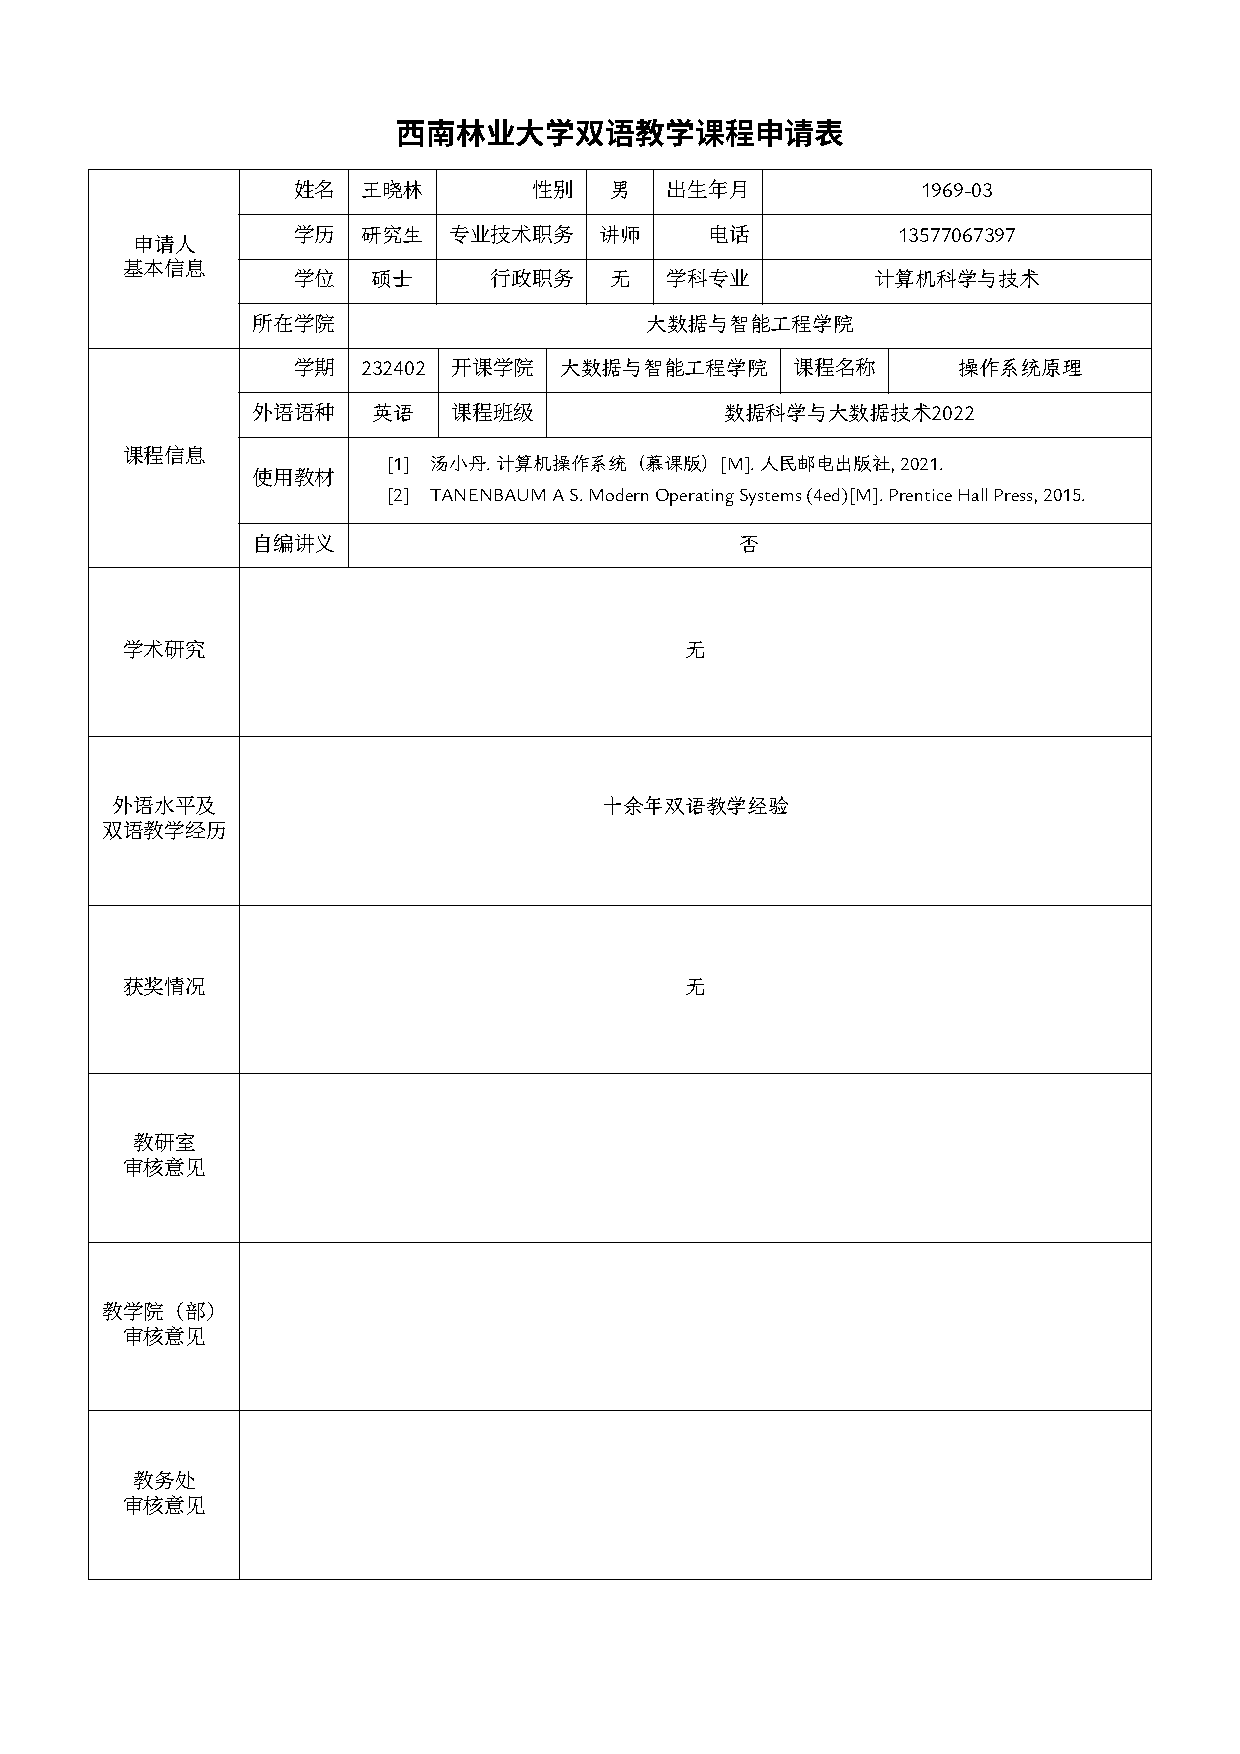
\includegraphics[width=.3\textwidth]{os}
  \bicaption{操作系统在计算机系统中的位置}{The position of an OS in the computer system}
  \label{fig:os}
\end{figure}

操作系统是计算机系统里运行的最重要的一个软件,如图~\ref{fig:os}所示,它是介于系统硬件
(Hardware)和各种应用程序(Application)之间的软件。任何应用程序如果想操纵系统硬件,都要经
过操作系统这一关。操作系统在计算机中的角色很类似现实社会生活中的政府,它是
\begin{itemize}
\item 资源管理者。所谓“资源”,笼统讲就是所有的系统硬件,包括CPU、内存、网卡、声卡、显卡、键
  盘、鼠标\ldots{}\ldots{}它们的共同特点就是``紧缺''。系统中的众多应用程序都要``抢用''这些
  硬件资源。操作系统要负责协调应用程序之间的资源竞争。当然,它本身也要消耗掉一部分系统资源
  以维持自身的正常运转。一个低消耗、高效率的政府才会受欢迎,操作系统也是一样。
\item 系统控制者。操作系统控制着系统中程序的运行,一旦发现有程序出错,或有程序非法使用系统
  资源,就要及时处理,以保障系统能安全、有序、高效地工作。
\item 公共服务提供者。比如上面说到的,所有硬件的驱动程序只要在操作系统里保留一份就可以了,
  不必要每个应用程序里都携带相同的驱动程序。
\end{itemize}

% 是系统资源的管理者,负责为用户管理所有的软件
% 和硬件资源,如用户进程、CPU、内存、硬盘,以及其它硬件设备。操作系统还为用户提供使用计算机的
% 接口,如图形界面,命令行解释器。有了这些接口,用户甚至都不用学习任何计算机语言,只要
% 动动手指点击一下按钮、图标、菜单或者敲几个命令就可以跟计算机交流了。可以这样说,如果没有操
% 作系统,一台计算机基本上就没什么用了。

自上世纪60年代分时系统诞生以来,时光已跨过了近50年。随着计算机硬件技术的突飞猛进,操作系统
这一和硬件形影不离、息息相关的软件,也发生着沧海桑田的巨变。1969年诞生的UNIX操作系统只有寥
寥4200余行代码,而今天它的分支系统已遍布天下。其中,Linux系统内核的代码量已超过了两千万行。
除了通常所见的计算机上的通用型操作系统之外,随着硬件技术和网络技术的发展,各种特殊用途的操
作系统也应运而生,如,手机系统、实时嵌入式系统、分布式系统、虚拟机、以及当下流行的云计算系
统等等。

Linux操作系统以其本身的开源性,以及低成本性,吸引了众多的公司为其提供技术支持,以及大量的自
由开发爱好者和开发开发社区为其贡献代码。Linux提倡的自由软件运动,让它迅速成为在业界中使用最
广泛的系统。另外,相比其他操作系统内核,Linux内核具有更快、更安全、更容易获得,和更灵活的特
点。Linux的开源性使得所有人都可以轻松获得源代码,并且可以按照自己的个人意愿随意更改内核。所
以,以Linux内核作为内核开发的学习模板,是最合适的选择。本文就是以Linux的最初版本为参考,
对操作系统的实现的一次初步探索。

操作系统的功能通常包括进程管理、中断处理、内存管理、文件系统、设备驱动、网络协议、系统安全、
输入输出等许多方面。其中进程管理部分提供了创建进程、运行进程、调度进程、和进程同步等功能。
内存管理部分的主要功能就是为进程提供一个内存的抽象,实现进程的虚拟地址空间,为进程分配内存
和回收内存。文件系统则主要负责数据在硬盘上的存储和组织方式,并为用户进程提供一个文件操作的
接口。现代操作系统最显著的特点就是实现多任务,因此负责实现多任务的进程管理和内存管理便成为
了内核研究领域中的重点。基于这一点,本文便以进程管理和内存管理作为研究的方向,并广泛学习内
核设计中关于进程管理与内存管理方面的知识,最后以Linux内核为学习模板,通过理论与实践相结合,
努力实现进程管理和内存管理的各项基本功能,并争取能有所创新。

\section{国内外研究现状}

\subsection{国外发展现状}

操作系统研发一直是计算机技术研究的重要领域,而操作系统的研发主要是围绕内核的研究来展开的。
内核的研究主要包含三方面:进程管理、内存管理和文件系统的研究。而进程管理和内存管理一直来都
是内核研究的热点。近年来,在操作系统研发领域中,发展势头最好的是以linux为内核的系统。据全
球Top500超级计算机发布数据显示,截止到2017年11月,100\%的超级计算机都在运行Linux操作系
统\footnote{\url{https://www.top500.org/statistics/list/}}。linux操作系统占据了全球90\%的云
计算服务器,并且在嵌入式系统占据了62\%的市场份额。linux在移动设备中也占据了80\%的份额。桌面
操作系统市场份额虽然没有服务器那么高,但也呈逐年扩大趋势。近年来,随着国际大公
司Intel、 Google、IBM、甚至微软等,都在Linux操作系统上加大研发投入,为Linux操作系统的长远发
展提供资金和技术支持。同时,Linux拥有众多的开发社区,这些开发社区均由来自世界各地的优秀内核
开发者组成,这些社区开发者为Linux内核的发展贡献了大部分的代码。现在Linux社区拥有大约15600个
来自世界各地的个人开发者和来自1400多个公司的技术支持。这使得Linux内核大概每9~10个星期就能
产生一个性能有所提升且稳定性良好的新版本。Linux内核研究发展的方向主要是围绕着如何提升系统的
运行速度这个问题而展开,其中包括了,如何更快速的让一个进程运行起来、如何更快速地进行进程切
换、如何更快速地处理中断、如何更快速地实现内存分配以及如何提高文件系统的访问速度等问题,而
这些问题都主要属于进程管理、内存管理模块和文件系统模块的功能。所以,Linux内核的研究直接推动
了作为内核主要部分的进程管理和内存管理模块的发展。

\subsection{国内发展现状}

从2001年以来,基于Linux的服务器操作系统逐步发展壮大。国内几个主要的Linux厂商和科研机构,国
防科技大学、中标软件、中科红旗等先后推出了Linux服务器操作系统产品,并且已经在政府、企业等领
域得到了应用。目前国内涉及的操作系统研发也主要是以Linux内核为模板,并在此基础上拓展一些新的
外围功能。目前国内发行的Linux 版本主要有:红旗、中标、共创、新华、拓林思等,均有桌面和服务
器两个版本;但是,国内各发行版均基于国际社区版本发展而来,是在基于国际社区的内核开发成果上,
只对操作系统的界面和外围软件做了一些改变,而实际上并没有掌握Linux的核心技术,基本上没有涉及
对Linux内核里的进程管理和内存管理,文件系统这三个功能模块的研发。所以,国产Linux系统与国
际Linux操作系统发行版之间存在比较大的技术差距。目前国内的Linux内核研究项目普遍存在着资金不
足,人才缺乏的问题。因此,国内操作系统研发组织机构、厂商也都相应加大资金和人力的投入,努力
做到能在内核的进程管理、内存管理和文件系统这些功能模块的发展上做出贡献,以缩小与国际 Linux
研究组织之间的差距。

\section{面临的问题}

几十年来,计算机科技一直在迅猛发展,CPU的运算速度越来快,内存的容量也越来越大。为了最大程度
地发挥计算机硬件的效率,软件技术也在不断地进步、创新,软件功能越来越复杂,软件的规模也越来
越庞大。庞大而复杂的软件总是需要更快的CPU和更大的内存来承载和运行。为了满足软件的需求,硬件
技术就要更上层楼。硬件技术的提高又为催生规模更大、功能更复杂的软件提供了肥沃的土壤。硬件和
软件之间的发展竞赛,一方面活跃了计算机产业,另一方面也带来了不小的问题。硬件水平却一直没有
能跟上软件发展的水平,在一个系统里,CPU数量远远少于要运行的软件数量,以及内存的尺寸远远小于
要运行的软件的尺寸,这两个问题还始终存在着。这些问题的解决仍然依赖于更有效的CPU调度算法和虚
拟内存技术。

本文在实验的过程中研究的主要问题有:
\begin{itemize}
\item 如何提高内核处理系统调用、异常、和中断的速度;
\item 在多个CPU的系统里,如何设计调度队列和调度算法;
\item 如何防止因用户传入的参数过大,导致用户栈的溢出问题;
\item 在内核代码与程序代码同处于一个地址空间内的情况下,如何防止用户程序随意访问或更改内核
  区域的问题等。
\end{itemize}

\section{本文研究内容}

现代通用型操作系统结构复杂、功能多样,现代操作系统的开发是一项庞大而复杂的软件工程。如
图~\ref{fig:overview}所示,操作系统内核包括文件系统、进程管理、内存管理、设备驱动、硬件控制、
系统调用等众多功能模块。其中任何一个内核模块的设计与开发都要求开发者具有极高的素质与经验,
对系统内部的总体架构、运行机制、模块间的衔接关系等有极其深入的了解。考虑到任务的复杂性,以
及时间和个人开发经验等方面的限制,在短期内独立完成上述诸多任务显然是不现实的。所以本文
以Linux内核为参考,着重研究探讨进程与内存管理方面的设计与实现。

进程管理是操作系统内核实现进程管理的一个模块,主要功能包括进程的创建、进程的运行、进程的调度和进程
间的同步几个部分。内存管理是操作系统内核管理内存这一个资源的一个模块,主要功能包括内存的格
局分布、进程空间的抽象、内存分配和回收以及虚拟内存技术。

\begin{figure}
  \centering
  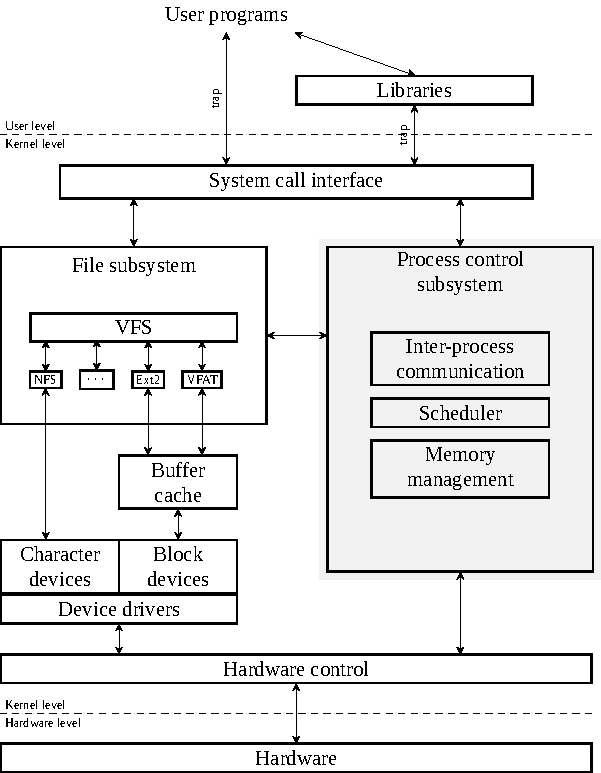
\includegraphics[width=\textwidth]{overview}
  \bicaption{操作系统内核概览}{OS overview}
  \label{fig:overview}
\end{figure}

\section{技术路线}

本文的目标是设计和实现操作系统内核中的进程管理和内存管理这两个模块的功能。主要研究如何快
速地创建进程、调度进程、切换进程,如何处理进程间的同步问题以及如何高效率地管理内存并为进程
分配空间、回收空间等内容。

本文以最为常见的Intel x86处理器为硬件平台。软件开发环境主要包括:
\begin{itemize}
\item Debian GNU/Linux 9 (4.14.0-3-amd64);
\item GCC编译器;
\item GDB调试器;
\item QEMU虚拟机。
\end{itemize}

在创建进程时,采用的是对象创建模式,用已有的对象创建新的对象,即所谓的母进程创建子进程。母
进程通过调用\texttt{fork()}函数,来完成如下一系列操作:
\begin{enumerate}
\item 为子进程分配一个进程控制块,PID号;
\item 分配内核栈;
\item 将母进程的物理内存空间与子进程共享;
\item 复制一份母进程打开的文件给子进程;
\item 为子进程提供写时复制的内存分配方法。
\end{enumerate}

在调度CPU时,所有CPU共享一个就绪队列,每个CPU都有一个自己的调度器,为了便于实现,所有的调度
器使用相同的调度算法:Round-Robin算法;在处理进程间的同步问题时采用两种不同的锁对不同性质的
共享资源提供保护。

在内存的存储管理方式上采用的是分页方式。对内存上的空闲页的管理采用的是地址池的方式。对新创建的
进程的初始地址空间的分配是采用的子进程共享母进程的内存空间,并在需要时进行页面复制的方法。
在给进程分配用户栈的时,采用额外分配一个空页的方法来防止用户栈的溢出。在进程需要重新映射地
址空间时,采取为进程重新分配并映射页表的方法。最后,在处理进程的运行时内存分配的问题上,采
取了延迟分配的方法来进一步节省内存开销。

\chapter{进程管理的设计与实现}

操作系统里最重要的概念之一是进程。进程可看作是对一个正在运行的程序的一个抽象。系统里的所有
工作都是围绕着这个概念而进行的。进程概念的引入,使系统得以在只有一个CPU的情况下也能够实现多
任务的并发执行。现代的通用计算机都要能满足同时做几件事的需求。举例来说,一个网页服务器在某
一个时间段内可能会收到很多个服务请求。服务器接收到一个请求之后,首先会查看缓存里是否已经存
有了用户请求得到的网页,如果有的话,则可直接给用户返回,如果缓存内没有的话,则需要从硬盘内
读取结果再将其返回给用户。进程在读盘的时候是用不到CPU的,而且读取硬盘是一个漫长的过程。如果
系统没有多任务并发机制的话,在某进程读取硬盘的时候,CPU就只能闲置,白白浪费了很多CPU的宝贵
时间。并且别的请求由于等待时间过长,可能会被撤出内存。为了解决这一个问题,计算机系统必须具
备处理并发事务的能力,通过把不同事务给模型化成一个个的进程加以控制管理。进程管理主要是解决
操作系统如何创建进程,调度进程,以及如何处理进程的同步问题。其中,进程的创建是指如何创建一
个新的进程,主要是通过\texttt{fork()}系统调用来完成。进程调度主要是让系统按照预先制定好的一
个或多个调度策略来调度进程,也就是利用调度策略的规则来决定谁是下一个能占用CPU的进程,从而实
现让多个进程以时分复用的方式共享CPU资源。进程同步则主要是解决多进程互相争夺共享资源时产生的
冲突。

\section{总体设计模型}

本设计的进程管理部分包括进程的创建、进程的终止、进程调度、进程间同步等四个功能模块。各模块
间的关系如图~\ref{fig:proc-top}所示。其中,
\begin{itemize}
\item 进程的创建主要解决的是如何对进程做出一个抽象的定义,如何定义进程的各种状态,如何存放
  进程以及如何用已有的进程创建新的进程等问题;
\item 进程的运行终止主要解决的是如何处理进程退出时资源的回收问题;
\item 进程的调度主要解决的是在多进程中如何合理分配CPU使用权的问题;
\item 进程间同步指的是如何避免多进程共同访问一个共享资源时出现竞争的问题。
\end{itemize}

\begin{figure}[h]
  \centering
  \begin{center}
    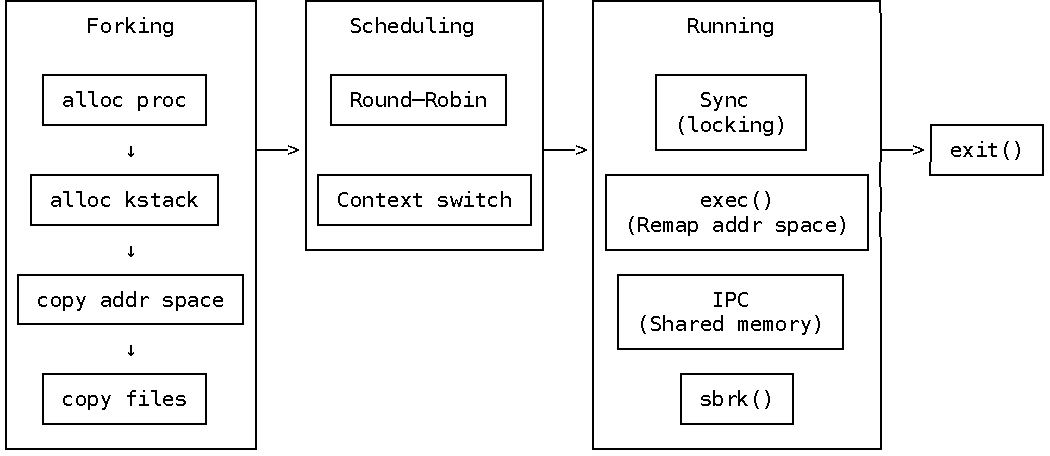
\includegraphics[width=.8\textwidth]{proc-top}
  \end{center}
  \bicaption{进程管理概要设计图}{Process management top-level design}
  \label{fig:proc-top}
\end{figure}

在后面的章节中,我们将详细探讨各功能模块的设计与实现。

\section{进程结构体的设计与实现}

进程是正在运行的程序的一个实例,是操作系统里最重要的概念之一。实际上,进程和程序间的区别是
微妙的。用一个比喻可以使我们更容易理解这一点。想像一位有一手好厨艺的计算机科学家正在为他的
女儿烘制生日蛋糕。他有做生日蛋糕的食谱,上面列出了所需的原料:面粉、鸡蛋、糖等,还有一个详
细的做蛋糕的步骤。在这个比喻中,做蛋糕的食谱就是程序(即用适当形式描述的算法),计算机科学
家就是处理器(CPU),而做蛋糕的各种原料就是输入数据。进程就是厨师阅读食谱取来各种原料以及烘
制蛋糕等一系列动作的总和。这里的关键思想是:一个进程是某种类型的一个活动,它有程序、输入、
输出以及状态。单个处理器可以被若干进程共享,它使用某种调度算法决定何时暂停一个进程,并转
而为另一个进程提供服务\cite{linuxjournal:process}。

在面向进程而设计的系统中,进程是程序的基本执行实体;在面向线程设计的系统中,进程本身不是基
本运行单位,而是线程的容器。进程可以分为系统进程和用户进程。凡是用于完成操作系统的各种功能
的进程就是系统进程,它们就是处于运行状态下的操作系统本身。用户进程是由用户自己启动的进程。
进程是操作系统进行资源分配的单位。在操作系统的设计中引入进程概念,可以方便地实现各任务之间
的彼此隔离。系统中的每个进程都运行在自己独立的虚拟地址空间中,因此每个进程都认为自己是系统
中唯一在运行的程序,并且拥有全部的系统资源,如CPU、内存
等\cite{Bryant2010computersystems,silberschatz11essentials}。

一个程序如果要运行,首先要由操作系统把它加载到物理内存当中。在程序加载的时候,操作系统负责
将该进程的虚拟地址空间映射到物理内存当中。虚拟内存地址与物理内存地址之间的映射关系会被保存
到页表(page table)中。操作系统负责进程之间的保护(也就是隔离),确保任何进程不能随意访问
其它进程的地址空间。逻辑地看,每个进程的私有虚拟地址空间都被划分为代码段、数据段、堆栈段、
以及进程状态段等若干部分,如图~\ref{fig:process}所示。

\begin{figure}[!htb]
  \centering
  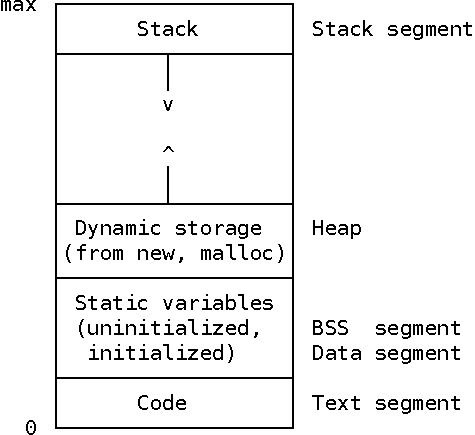
\includegraphics[width=.6\textwidth]{process}
  \bicaption{进程的逻辑结构}{Process logical view}
  \label{fig:process}
\end{figure}

\subsection{进程的地址空间}\label{sec:procvm}

虚拟地址空间,或者也叫地址空间,是操作系统所能提供给进程的虚拟地址的范围\cite{zos}。
每个进程的虚拟地址空间的大小都与CPU所能寻址的最大空间相当。以32位系统为例,每个进程的虚拟地
址空间大小为$2^{32}=4\,G$。4G空间被分成两部分,高位部分地址用于映射操作系统的内核空间,低
位部分地址用于用户空间的数据和代码映射。传统的Linux系统一般将进程的虚拟地址空间划分为1G:3G,
其中1G做为内核空间映射,3G用做用户空间\cite{silberschatz11essentials}。本实验系统采用的
是2G:2G的划分,即从0\char`~2G的地址是用户空间,2G\char`~4G为内核空间。进程的虚拟地址空间如
图~\ref{fig:process-vm}所示。之所以采用2G:2G的划分,是因为考虑到本文是以探讨内核开发为主,
理应为内核留出更为充裕的空间。

\begin{figure}[!htb]
  \centering 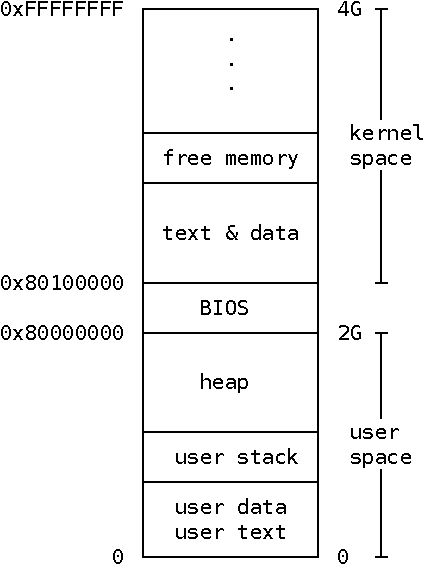
\includegraphics[width=.5\textwidth]{proc-vm}
  \bicaption{进程虚拟地址空间}{Process virtual memory space}
  \label{fig:process-vm}
\end{figure}
 
在现代流行的操作系统的设计中,通常都是把内核工作空间完整地映射到每个进程的虚拟地址空间
里\cite{love2010linux}。这样做的好处是,进程在请求内核服务时(如system call的调用),内核代
码直接运行在当前进程的地址空间之内,不需要进行进程的切换,不需要改换地址空间,节省了很多的
上下文切换的时间,只需切换到内核模式即可运行内核代码。

\subsection{进程状态与进程控制块}
\label{sec:proc}

进程控制块(Process Control Block)也叫任务控制块,是为了方便管理进程而在系统内定义的一个数
据结构,用来存放进程相关的各种信息,包括进程所占用的内存大小信息,页表信息,状态信息,进程
身份ID,进程名称,当前工作目录,以及进程打开的所有文件文件等信息。系统对进程的操作都是通过
对进程控制块的读写来完成的\cite{silberschatz10java}。其中,进程的状态包括:

\begin{description}
\item[embryo:] 是进程刚被创建时的状态。
\item[runnable:] 是指进程已经处于具备了一切可运行的条件的状态。
\item[running:] 是指进程正在运行的状态。
\item[sleeping:] 是指进程因为等待某种条件或事件而放弃CPU使用权而进入的睡眠状态。
\item[zombie:] 是指进程已经运行结束了,但是所占资源尚未被完全回收时的状态。
\end{description}
以上各进程状态之间的转化关系如图~\ref{fig:pstates}所示。

\begin{figure}[!htb]
  \centering
  \vspace*{2ex}
  \begin{center}
    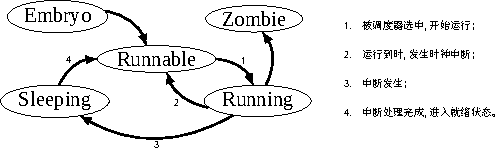
\includegraphics[width=.8\textwidth]{pstates}
  \end{center}
  \bicaption{进程各状态之间的转化关系}{Process state transition}
  \label{fig:pstates}
\end{figure}

在本项目中,进程控制块被定义为一个结构体(struct),名为\texttt{proc},其内容如程
序~\ref{lst:proc}所示。

\begin{listing}
  \begin{codeblock}
\begin{ccode}
struct proc {
  uint sz;                 // 进程空间大小
  pde_t* pgdir;            // 页表起始地址
  char *kstack;            // 内核栈起始地址
  enum procstate state;    // 进程的六种可能状态
  int pid;                 // 进程号
  struct trapframe *tf;    // 位于内核栈中,用来保存trap发生时的寄存器的值
  struct context *context; // 指向进程的上下文
  void *chan;              // 如果非0,则进程位于sleeping队列里
  struct file *ofile[NOFILE]; // 进程打开的文件
};
\end{ccode}
  \end{codeblock}
  \bicaption{\texttt{proc}结构体}{\texttt{struct proc}}\label{lst:proc}
\end{listing}

为了便于统一管理系统中存在的所有进程,创建一个\texttt{proc[64]}数组,用来存放所有的进
程。\texttt{proc[64]}数组是所有的CPU所共享的。为了防止两个或多个CPU因同时访问它
而引起冲突,在这里我采取了给\texttt{proc[]}数组加锁的方法,于是就定义了一个叫\texttt{ptable}的结构体,
如程序~\ref{lst:ptable}所示。\texttt{ptable}、\texttt{proc[]}数
组、与\texttt{proc}结构体三者之间的关系如图~\ref{fig:ptable}所示。

\begin{listing}%[H]
  \begin{codeblock}
\begin{ccode}
struct {
  struct spinlock lock; //用于保护proc数组的锁
  struct proc proc[NPROC];
} ptable;
\end{ccode}
  \end{codeblock}
\bicaption{\texttt{ptable}结构体}{\texttt{struct ptable}}\label{lst:ptable}
\end{listing}

\begin{figure}[!htb]
  \centering
  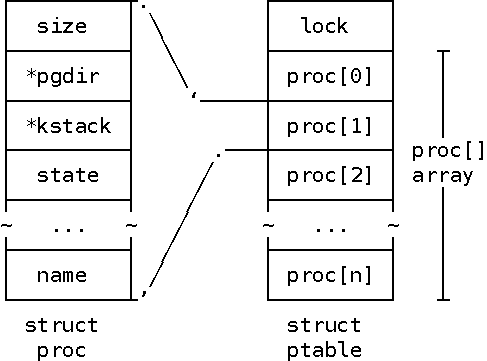
\includegraphics[width=.6\textwidth]{ptable}
  \bicaption{\texttt{ptable},\texttt{proc[]}数组,与\texttt{proc}结构体}{\texttt{ptable,
      proc[]}, and \texttt{struct proc}}
  \label{fig:ptable}
\end{figure}

由于\texttt{ptable}是多进程都可以同时访问的公共数据块,这意味着若干进程有可能同时读写该结构体。
为了避免同时读写而发生的冲突,就需要引入一个加锁保护机制。进程只有在取得锁之后才能读写该公共
结构体。关于加锁机制的实现,在后面的第~\ref{sec:lock}节有详细讨论。

\subsection{内核栈}

进程运行在用户态的时候,函数调用使用的是用户栈(user stack)。当进程进入内核态运行的时候,如
果还继续使用用户栈的话,就会降低系统的安全性。因为,在栈顶处存放的数据未必是合法的,有可能
是用户进程产生的非正确的数据,甚至有可能遇上恶意进程存放的非法地址,如别的进程的地址,专门
诱导内核为它做非法访问。为了避免这些危险,进入内核态运行时必须要有专门的内核栈(kernel
stack)以供函数调用时使用\cite{stack:kernelstack}。进程在内核态与用户态之间切换时,必须进行
栈的切换。进程在新创建时,由\texttt{allocproc()}函数(附录~\ref{sec:allocproc})为其分
配一个内核栈。内核栈主要用来存放\texttt{trapframe}和进程的上下文(context)。其
中,\texttt{trapframe}(附录~\ref{sec:trapframe})是在系统响应中断时,内核栈中专门用来保护
现场(即保存相关寄存器)时用的一块区域\cite{stack:kernelstack2}。\texttt{context}则是进程切
换时,内核栈中专门用来存放与进程的上下文相关的寄存器的一块区域。

% \subsection{异常、系统调用、和中断}

% 进程在运行时,一般情况下,都是CPU在逐行读取程序代码,并运行程序指令。但是当一些特殊情况发生
% 时,这种情况便会被打断,CPU必须暂时停止该进程的运行,转而执行一些相应的内核代码来处理这些特
% 殊情况。这些特殊情况包括:异常、系统调用、以及中
% 断\cite{tanenbaum2008modern,silberschatz11essentials}。其中,异常是指程序运行过程中产生的错
% 误,如CPU在运行的过程中出现除数为0的错误、溢出错误、边界检查错误、缺页错误等。系统调用是内核
% 提供给用户进程的一套服务接口,这个接口里包含了一系列的函数,用户进程通过调用这些函数来请求
% 内核提供服务,如读写硬盘、创建子进程、打开文件、获取pid号等具体事
% 务\cite{stevens2013advanced}。中断则是指硬件设备向CPU发送的一个请求内核服务的信号,如系统时
% 钟向内核发出信号,提醒内核该进行进程切换或者是硬盘向内核发出信号以告知内核自己已读完数据了
% 等等来自设备的事件。

% 进程在运行的过程中,遇到以上这三种情况时,CPU的工作便被打断,暂时停止用户进程的指令然后对这些情
% 况做出相应的处理,即根据情况选择运行相应的异常处理函数/系统调用处理函数/中断处理函数。在运行完相应的内
% 核处理函数后,CPU便会切换回用户模式,继续运行用户进程的指令。在x86系统里,由于系统调用与异
% 常情况的发生,最终都与中断的发生过程相似,即都是通过执行一条\texttt{INT}中断指令来陷入内
% 核,然后根据中断号来查询IDT表找到相应的处理函数入口地址的,所以,对系统调用与异常这两种情况
% 的处理流程,也与普通的硬中断的处理流程类似,因此在本实验中,为了方便起见,这三种情况统一被
% 称为Trap。进程在运行的时候,如果遇上trap的话,CPU会进入内核态,把当前进程的运行状态保存在
% 属于进程的内核栈的trapframe区域中,然后运行相应的trap处理程序,在trap处理程序运行结束后,
% CPU会切换回用户态,继续运行用户进程。接下来将以系统调用为例,说明trap发生后系统的处理流程。

% x86架构提供了四种CPU工作模式,标号0\char`~3。在实际中,最常用到的却只有两种模式,0号和3号,
% 即内核模式也叫内核态与用户模式也叫用户态\cite{duarte:cpu-ring}。CPU当前的工作模式被保存
% 在cs寄存器内。中断描述符表(IDT),是专门用来存放所有的中断处理程序的入口地址的一个数组,所
% 有的系统调用,异常以及中断的处理程序入口地址都被保存在这个数组中。这个数组一共有256个入口,
% 每一个入口存放一个中断处理程序的入口地址(段地址和段内偏移)和执行时所需的权限。内核以数字
% 来区分这256个中断,其中0\char`~31号指向所有处理因程序产生的异常情况的函数的入口地址,
% 而32\char`~63号中断指向所有设备产生的硬中断处理函数的入口地址,64号中断则指向存放所有系统调
% 用处理函数入口地址的一张表格(系统调用表)\cite{bovet2005understanding}。

% 系统调用发生的主要过程如图~\ref{fig:syscall-read}所示。该图以POSIX系统中调用
% \texttt{read()}函数为例,说明了系统调用的大致过程\cite{tanenbaum2008modern}。  

%  \begin{figure}[!htb]
%    \centering
%    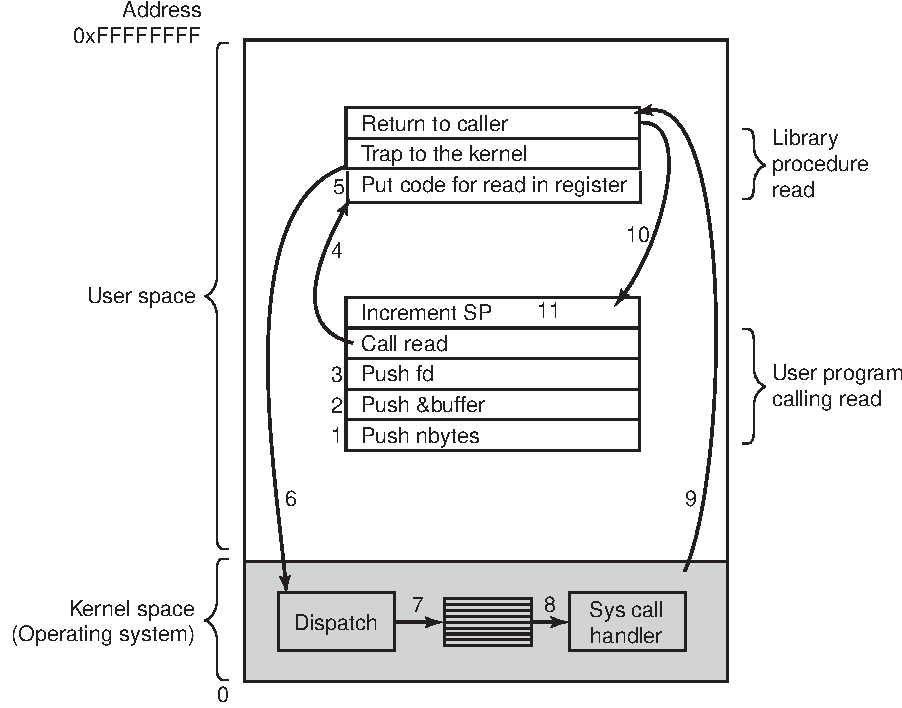
\includegraphics[width=.8\textwidth]{syscall-read}
%    \caption{系统调用示例(用户进程调用\texttt{read()}函数)}
%    \label{fig:syscall-read}
%  \end{figure}

%  当用户进程需要从某文件中读取数据的时候,便要在程序里调用\texttt{read(fd, buffer,
%    bytes)}库函数,表示需要从文件描述符为\texttt{fd}的文件起始位置开始,向后读
%  取\texttt{bytes}这么多字节的数据,并将读出的数据保存到内存中预先分配好的一
%  个\texttt{buffer}内。用户进程调用\texttt{read()}函数的系统的处理过程大致如下:

%  \begin{enumerate}
%  \item 用户进程把库函数需要的参数按照反序压栈;
%  \item 执行库函数\texttt{read()}中的指令代码;
%  \item 库函数把系统调用号放入eax寄存器;
%  \item 库函数执行\texttt{int}指令,CPU切换入内核模式;
%  \item 对内核栈里的\texttt{trapframe}区域进行设置;
% %  \item 从任务状态段中加载进程内核栈的esp寄存器和ss寄存器;
% %  \item 把当前进程的ss寄存器和esp寄存器压栈;
% %  \item 把当前进程的段寄存器,指令指针寄存器压栈;
% %  \item 把当前进程的eip指针压栈;
% % \item 把中断号压栈;
% % \item 把ds、es、fs、gs寄存器压栈;
% \item 根据中断号查询IDT得出系统调用表的入口地址;
% \item 根据系统调用号查询系统调用表得出对应的系统调用处理函数的入口地址;
% \item 开始运行系统调用处理函数;
% \item 系统调用处理函数返回,把结果留在eax里;
% \item 进程切换回用户态;
% \item 库函数把系统调用返回值交给用户程序。
% \end{enumerate}
% 其中,内核对\texttt{trapframe}(附录~\ref{sec:trapframe})的设置主要是通过保存一系列与运行
% 现场相关的寄存器来实现的,如保存进程的用户堆栈段指针和栈顶指针、段寄存器、eip寄存器等。在内
% 核完成对\texttt{trapframe}的设置后,一个进程的内核栈的主要内容如图~\ref{fig:kstack}所示。
  
% \begin{figure}%[!htb]
%   \centering
%   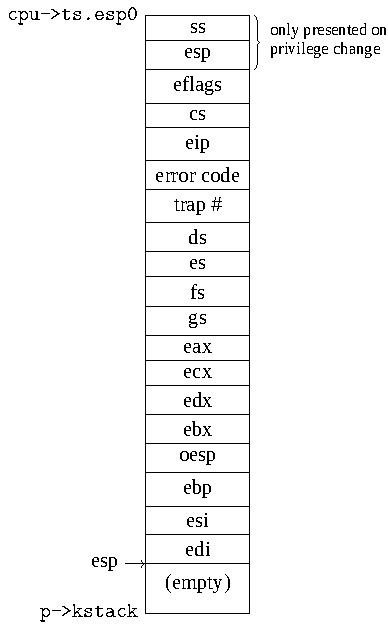
\includegraphics[width=.4\textwidth]{kstack3}
%   \caption{内核栈}
%   \label{fig:kstack}
% \end{figure}

%trapframe的定义如程序~\ref{src:trapframe}所示。
% \begin{listing}[H]
%   \begin{codeblock}
%   \end{codeblock}
%   \caption{\texttt{trapframe结构体}}\label{src:trapframe}
% \end{listing}

%\paragraph{INT指令}
% x86架构提供了四种CPU工作模式,标号0\char`~3。在实际中,最常用到的却只有两种模式,0号和3号,
% 即内核模式与用户模式。CPU当前的工作模式被保存在cs寄存器内。中断描述符表(IDT),是专门用来
% 存放中断处理程序的入口地址的一个数组,所有的系统调用,异常以及中断的处理程序入口地址都被保
% 存在这个数组中。这个数组一共有256个入口,每一个入口存放一个中断处理程序的入口地址(段地址和
% 段内偏移)和执行时所需的权限。内核以数字来区分这256个中断,其中0\char`~31号指向所有因程序产
% 生的异常情况处理函数的入口地址,而32\char`~63号中断指向所有设备产生的硬中断处理函数的入口地
% 址,64号中断则指向存放所有系统调用处理函数入口地址的一张表格(系统调用表)\cite{bovet2005understanding}。\texttt{INT}中
% 断指令所需完成的工作如下:

% \begin{enumerate}
% \item 以中断号为索引,从IDT表里读取相应的门描述符;
% \item 检查当前进程的CPU模式级别是否大于请求的中断门所要求的模式级别;
% \item 如果上一步成立,则需从任务状态段中加载esp寄存器和ss寄存器,供内核使用;
% \item 如果上一步成立,则将当前进程的用户堆栈段寄存器ss与栈顶指针寄存器esp压入栈中;
% \item 将当前进程的eflags寄存器压栈;
% \item 将当前进程的cs寄存器 压栈;
% \item 将当前进程的eip寄存器压栈;
% \item 如果是异常中断,则将一个出错码(error code)压栈;
% \item 从IDT表里加载eip和cs寄存器的值;
% \item 转入中断处理函数运行。
% \end{enumerate}

\section{进程的创建与运行}
\label{sec:proc-creation}

创建一个进程,要先明确一个进程由哪些部分组成。这就如同要定义一个类(class),得先搞清楚它具
有哪些属性,以及相对应的操作等。对进程的创建也是如此。程序要变成一个进程,不仅要被加载入物
理内存,还要被分配一个全局唯一的身份号(PID),还要有名称,工作目录,以及运行、睡眠、退出等
等一系列的属性和状态。于是,可以抽象地把进程定义为一个具有以上所述属性的\texttt{proc}数据结
构。\texttt{proc}的具体定义参见第~\ref{sec:proc}节中所述的\texttt{proc}结构体。

由于每个进程的虚拟地址空间里都包含了对内核空间的映射,为了安全起见,防止恶意进程在用户栈内设
置非法地址,所以当进程进入内核模式运行时,必须另外有一个内核栈,供函数进入内核模式时使用而
不是继续使用用户栈。于是,在创建进程的时候,得首先给它从\texttt{ptable}里申请到一个空
的\texttt{proc}结构体,然后为其创建一个内核栈。在本项目里,这两个工作是通过\texttt{allocproc()}函数(附
录~\ref{sec:allocproc})来完成的。\texttt{allocproc()}的主要
工作流程如下:
\begin{enumerate}
\item 从头开始遍历\texttt{ptable}中的\texttt{proc[]}数组,从中找到的第一个进程状态
  为\texttt{unused}的数组单元即为可用单元;
\item 把找到的空单元格的进程状态设置为\texttt{embryo},表示初步占用;
\item 为新进程分配一个进程号;
\item 为新进程分配一个内核栈;
\item 在内核栈里预留一片\texttt{trapframe}大小的空间供\texttt{trap}发生时保存寄存器用;
\item 为\texttt{trap}的返回值预留一定空间;
\item 为保存进程上下文(\texttt{context})预留一定空间;
\item 设置上下文内的\texttt{eip}指针让其指向\texttt{fork()}函数的返回处。
\end{enumerate}

\subsection{\texttt{fork()}函数}

在创建进程的时候,我采用的是用已有的进程创建新进程的方法,即母进程通过调用\texttt{fork()}函
数来创建子进程。由于系统里的第一个进程(\texttt{initcode})没有母进程,所以是由内核自己创建的,后来的进程都是由
母进程通过调用\texttt{fork()}函数来创建。其中,调用\texttt{fork()}的进程为母进程,
用\texttt{fork()}创建的进程为子进程。并且子进程在被创建时,复制了母进程的地址空间、进程状
态、和打开的文件等内容。子进程创建完毕后,母进程继续完成它剩下的工作,而子进程则按照被创建
的需求完成相应的工作。由于\texttt{initcode}是系统里的第一个进程,所以它可以被看成是其他所有
进程的``始祖''进程。\texttt{fork()}函数(附录~\ref{sec:fork})的工作流程如下:
\begin{enumerate}
\item 调用\texttt{allocproc()}函数为子进程申请到一个\texttt{proc}结构体并分配一个内
  核栈;
\item 为子进程分配页表并映射内核空间;
\item 将母进程的用户地址空间重复映射到子进程的页表中;
\item 复制母进程的进程状态给子进程;
\item 把母进程的内核栈里的内容复制到子进程内核栈内;
\item 把子进程中\texttt{trapframe}里\texttt{fork()}函数的返回值置为0;
\item 把母进程打开的文件列表复制一份给子进程;
\item 把子进程的运行状态改为就绪(\texttt{runnable});
\end{enumerate}

\subsection{创建系统中的第一个进程}

系统里第一个进程是\texttt{initcode}进程,它是由内核直接创建的,主要负责启动命令行(shell)。
由于它没有母进程,自然不能通过调用\texttt{fork()}函数来创建,因此也就没有母进程
的\texttt{trapframe}和上下文(\texttt{context})可供复制。所以,内核要对系统中第一个进程的
创建做特殊处理,单独给它设置好内核栈里的\texttt{trapframe}和上下文
(\texttt{context})\cite{wang2004i386boot}。\texttt{initcode}进程的创建工作是通过调
用\texttt{userinit()}函数来完成的。在内核的主函数(\texttt{main()})完成对硬件的初始化工作
后调用\texttt{userinit()}函数来创建第一个进程。\texttt{userinit()}函数所
需完成的工作主要包括:
\begin{enumerate}
\item 调用\texttt{allocproc()}函数为新进程在\texttt{ptable}中的\texttt{proc[]}数组里分配一
  个空的数组单元,为其分配一个内核栈,并设置好进程的状态信息;
\item 调用\texttt{setupkvm()}函数为进程创建页表并映射内核空间;
\item 调用\texttt{inituvm()}函数为进程分配一页物理空间并把进程的二进制代码文件复制到这个空间里;
\item 设置进程的\texttt{trapframe}里的段寄存器的值;
\item 设置栈顶指针指向进程地址空间的最大值处(即用户栈处);
\item 设置指令指针指向地址0处(二进制代码的开始处);
\item 设置进程的名称为\texttt{initcode};
\item 把进程的运行状态从\texttt{embryo}改为\texttt{runnable};
\end{enumerate}

在\texttt{userinit()}函数完成\texttt{initcode}进程的创建并把它置为\texttt{runnable}之后,该
进程就进入了系统调度队列,可以接受调度运行了。

\section{进程调度与算法实现}

现代操作系统的重要特征就是支持多任务 ─ 即在系统内“同时”运行多个进程。所谓的“同时”,在这里
应被理解为时分复用。一个CPU在任何时刻下只能运行系统里的某一个进程。但是,系统里却存在多
个要执行的任务,为了解决这个问题,目前最常用的解决方案就是把CPU分时使用,即多个进程分时轮流
占用CPU。比如一个进程占用10ms之后,换成另外一个进程执行10ms,然后再换成别的进程执
行10ms,\ldots{},其中每个进程一次能占用CPU的时长就称为时间片(Time quantum),这就是所谓的
多任务并行。对于如何在多个任务中分配CPU的使用权,就需要制定一套相应的调度策略,也就是调度算
法。调度算法的设计需要考虑的问题有:系统的吞吐率、响应时间、最低延迟、和最大化公
平\cite{bach1986design}。在实践中,这些目标经常是互相冲突的,因此,调度策略需要实现一个权衡
利弊的折中方案,而侧重点则可能是前文提到的任何一种,这取决于用户的需求和目的。

\subsection{调度算法}

调度算法设计的基本原则是避免进程“饥饿”,也就是让所有进程都有使用资源的机会,并保证使用资源多方
的公平性。调度策略需要解决在大量请求下如何分配资源的难题。调度算法种类很多,最常使用的几种
主要有:先入先出(FIFO)、最短进程优先(SJF)、时间片轮转法(RR)和基于优先级的(OPT)算法。
这几种算法各有优点,同时也各有不足。例如FIFO算法,虽然实现起来简单,但是,如果遇
到一大堆短进程出现在长进程的后面的情况的话,就会导致进程的平均等待时间过长。而OPT算法则容易
出现进程饥饿的情况,即就绪队列里那些优先级较低的进程可能一直没有机会执行。% 当然,也可以通过
% 按照进程已等待时间长短来提升进程的优先级来解决这个问题,即随着进程的等待时间变长,进程的优
% 先级会提高。
时间片轮转(RR)算法设计简单,执行有效,又能实现公平性,所以使用广泛,所以,
在本项目里我采用的是这种调度算法。

\subsubsection{时间片轮转法(RR)}

RR算法的主要思想是,规定一个定长的时间片,就绪队列里的进程按照先来后到的顺序轮流使用CPU,在
时间片用完时,不管进程是否已经执行完了,都得把CPU使用权让出给下一个进程。下一个进程同样是占
用CPU达一个时间片长,然后再让出CPU给下一个进程,如此循环往复。此算法的特点是:算法的实用性
取决于时间片的长度,如果时间片定义得太长,则会延长系统对进程的响应时间,甚至变回先来先服务
算法;而如果把时间片定义得太短的话,虽然提高了系统对进程的响应时间却会导致频繁切换进程,从
而增加系统的开销,因为系统每次进行进程的切换,都要在切换上下文上花掉一部分时间,降低CPU的使
用效率。因此时间片的定义既不能太长也不能太短。在本项目中,时间片的大小定为10ms。

\subsection{进程切换的实现}

进程的切换是指操作系统系统暂停当前占用CPU的进程,利用调度算法从就绪队列里选择另外一个符合条
件的正在等待的进程,并把CPU交给它使用。进程切换机制使得共存于内存中的多个进程能共享CPU,是
操作系统实行多任务的手段。进程切换包括保存当前运行进程的上下文,选择下一个进程,切换页表,
加载新进程的上下文等几个步骤。

\subsubsection{进程的上下文}

进程的上下文(context)是进程运行状态的静态描述(快照)。具体地说,进程上下文包括计算机系统
中与执行该进程有关的各种寄存器(例如通用寄存器,程序计数器等)的值\cite{Sibasankar2010}。本实
验中进程上下文(\texttt{context})的定义如程序~\ref{lst:context}所示。
\begin{listing}%[H]
  \begin{codeblock}[.5]
    \begin{ccode}
struct context {
  uint edi;
  uint esi;
  uint ebx;
  uint ebp;
  uint eip;
}
\end{ccode}
  \end{codeblock}
  \bicaption{\texttt{context}结构体}{\texttt{struct context}}
  \label{lst:context}
\end{listing}

\subsubsection{进程的切换}

由于系统中CPU的数量(通常只有一个)少于进程的数量,所以为了保证所有进程都能使用到CPU,就要
进行进程的切换。进程的切换就是进程的上下文切换(context switch)。在三种情况下需要进行进程
的切换\cite{silberschatz11essentials}:
\begin{enumerate}
\item 进程运行完毕;
\item 进程阻塞;
\item 时间片用完。
\end{enumerate}

进程在切换时, 如图~\ref{fig:switch}所示,显然必须要让出CPU的使用权。其中,第一种和第二种情
况都属于进程主动放弃CPU使用权,而第三种情况属于进程不得不放弃CPU使用权。

\begin{figure}[h]
  \centering
  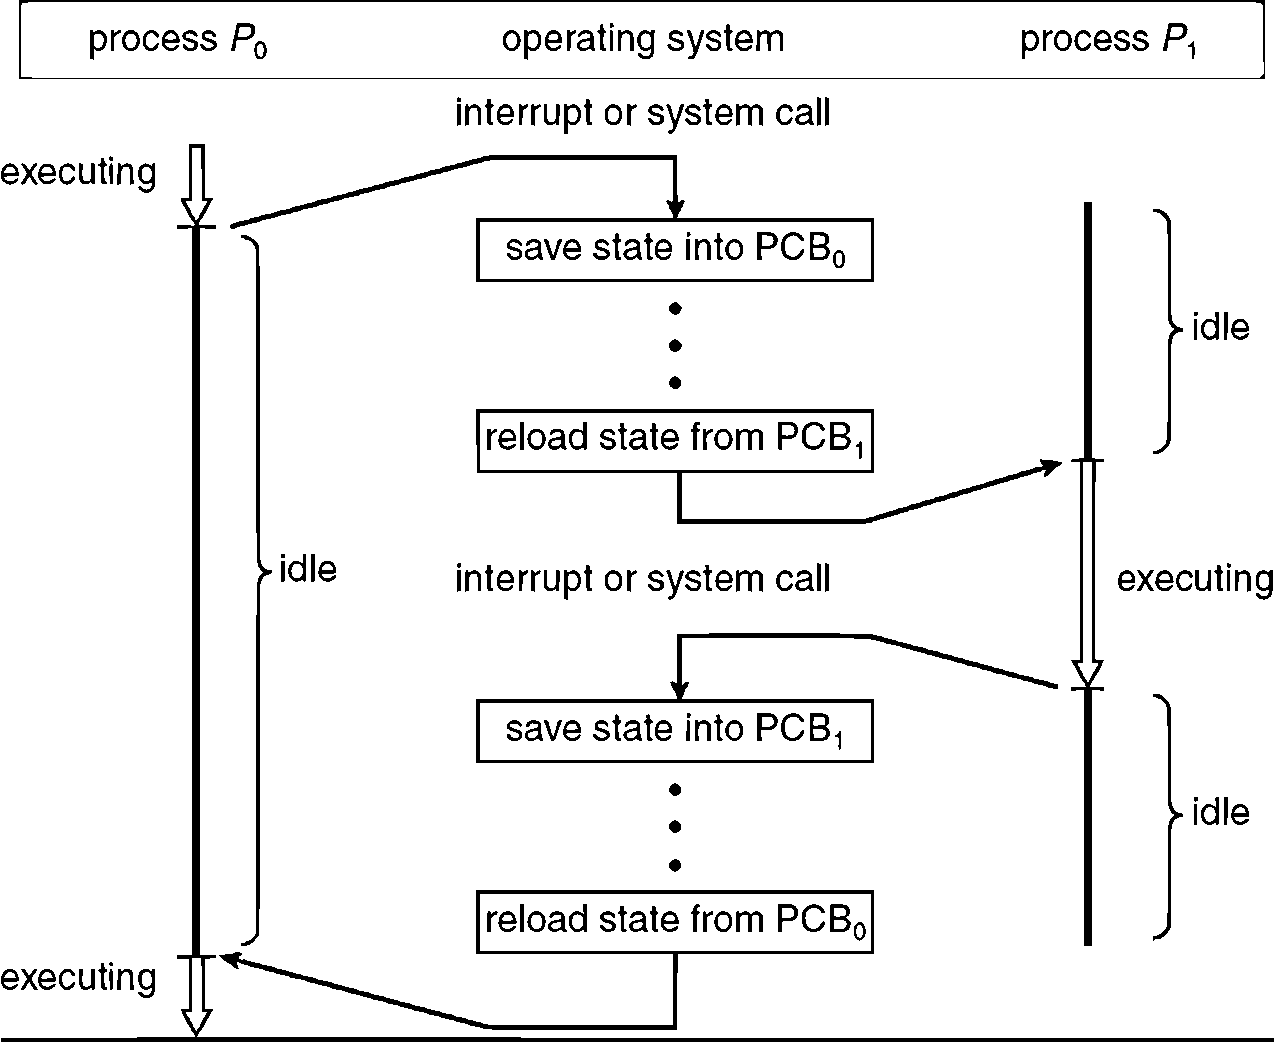
\includegraphics[width=.6\textwidth]{switch}
  \bicaption{进程的切换过程}{Process context switch}
  \label{fig:switch}
\end{figure}

进程切换时不仅需要切换跟进程相关的整套资源信息,包括地址空间的切换和上下文的切换,还需要运
行调度程序。其中地址空间的切换是通过改变页目录表(page directory)来实现的,而上下文的切换
则是通过保存当前进程的寄存器的值和恢复新进程的寄存器的值来实现的。本设计中,进程切换的大致过程如下:
\begin{enumerate}
\item 当前进程如果工作在用户态则先切换入内核态;
\item 当前进程保存eip,eax,edx寄存器的值;
\item 当前进程把参数(当前进程的上下文和将要运行的进程的上下文)压栈;
\item 当前进程调用上下文切换函数\texttt{swtch()};
\item \texttt{swtch()}函数继续把当前进程的寄存器压栈保存;
\item 切换到将要运行进程的内核栈;
\item 弹出将要运行进程的上下文寄存器的值;
\item \texttt{swtch()}函数返回。
\end{enumerate}

其中,\texttt{swtch()}函数(附录~\ref{sec:swtch})的工作内容主要是,把当前进程的上下文中用
到的寄存器的值保存起来,然后切换到下一个要运行的进程的内核栈,再把该内核栈中进程上下文里的
寄存器弹出就可以返回了。

\subsection{调度算法的实现}

本实验采用的调度算法是时间片轮转(RR)算法,其设计的主要思想是:从就绪队列的开头开始往下寻
找第一个进程状态为\texttt{runnable}的进程,找到后把CPU使用权交给该进程。在下一次调度的时候
便从该进程的位置开始往下寻找下一个\texttt{runnable}的进程……如此下去,如果搜索到了就绪队列的
最后一个位置仍然没有找到一个\texttt{runnable}的进程后便回到队列的开头,从头开始搜索。

调度函数(\texttt{scheduler()})也叫调度器,其主要工作是,
\begin{enumerate}
\item 按照规定好的调度算法来寻找下一个状态为\texttt{runnable}的进程;
\item 找到后,便把该进程设置为CPU的当前进程;
\item 调用\texttt{switchuvm()}函数切换到该进程的虚拟地址空间;
\item 把当前进程的状态改为\texttt{running};
\item 调用\texttt{swtch()}函数切换到该进程的上下文后进程便可开始运行了。
\end{enumerate}
值得一提的是,调度器自始至终都没有运行结束返回,实际上在内核启动时完成了对CPU的初始化工作之
后,调度器就启动了。调度器运行起来后,本身就是一个内核进程,而且拥有自己的栈,这使得当前进
程在让出CPU使用权时,实际上是先通过上下文切换到Scheduler进程的上下文,并把把CPU使用权交给
它。Scheduler进程拿到CPU使用权后便开始了寻找下一个符合运行条件的进程,然后进行上下文切换,
把CPU使用权交给该进程。在本项目里,调度器的实现是通过(\texttt{scheduler()})函数(附
录~\ref{sec:scheduler})来完成的。在进程切换的整个过程中,当前进程
(A)、\texttt{scheduler}进程、和下一个进程(B),这三者间的关系如图~\ref{fig:swtch}所示。

\begin{figure}[ht]
  \centering
  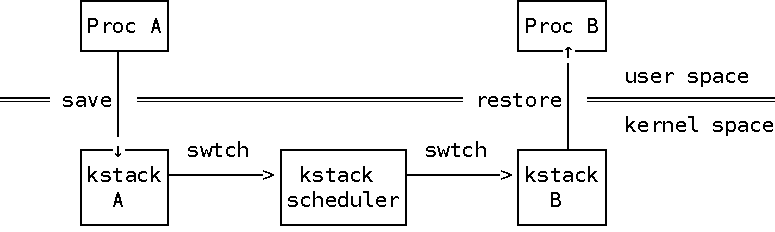
\includegraphics[width=.6\textwidth]{swtch}
  \bicaption{进程切换}{Process switch}
  \label{fig:swtch}
\end{figure}

\section{进程的退出}

一个进程在创建后便开始运行,以完成自己的使命。然而,没有什么是永恒的,哪怕是一个进程也不例
外。久而久之,进程终会终结退出。一个进程退出的原因主要有如下三个方面:
\begin{itemize}
\item 运行结束的正常退出;
\item 运行过程出错而退出;
\item 被另外的一个进程杀死而被迫退出。
\end{itemize}

当一个进程运行结束时,它并不能立即从系统中消失。事实上,在一个进程调用\texttt{exit()}函数退
出时,它先转入\texttt{zombie}状态,直到其母进程为其释放了进程空间,以及回收其占用的进程控制
块数据结构(\texttt{proc})后才算真正退出。如果进程的母进程在其退出之前已经先行退出了的话,
则由超级母进程(\texttt{initcode})负责释放和回收其占用的空间\cite{ArpaciDusseau14-Book}。
进程在彻底退出系统前需要完成一系列的退出准备工作\cite{mauerer2008professional},如:
\begin{enumerate}
\item 关闭该进程打开的所有文件;
\item 唤醒正在等待的母进程;
\item 把那些尚未运行结束或者已运行结束但不愿意为其完成资源回收工作的子进程交给\texttt{initcode}进程处理;
\item 把进程自己的状态设置为\texttt{zombie}态;
\item 把CPU使用权交给Scheduler以调度下一个进程。
\end{enumerate}

当进程通过\texttt{exit()}函数(附录~\ref{sec:exit})把正在等待的母进程唤醒后,母进程的状态便重新变
为\texttt{runnable}态,不久后将会被调度器选中。当母进程再次得到调度并运行起来后,会执
行\texttt{wait()}函数(附录~\ref{sec:wait})来回收子进程所占用的资源。其主要的工作过程是:
遍历\texttt{ptable}中的\texttt{proc[]}数组,寻找一个母进程为当前进程的进程,
\begin{itemize}
\item 如果找到了,则查看其状态是否为\texttt{zombie}态,
  \begin{itemize}
  \item 如果是,则记录其进程号(pid);释放其内核栈及其整个地址空间;然后再将其所占用
    的\texttt{proc}结构体清空;将其进程号返回给系统;
  \item 如果不是,则说明此进程尚未运行结束。跳过它,继续向下寻找。
  \end{itemize}    
\item 如果没有找到任何一个子进程,则返回-1;
\item 如果找到一个或若干个子进程,但都尚未运行结束,则让当前进程进入睡眠状态,以等待其中一
  个子进程运行完毕后将其唤醒。
\end{itemize}

在进程退出的整个过程中,\texttt{exit()}函数所能做的工作只是释放进程所占用的文件资源,即关闭
所有打开的文件。而进程所占用的其他资源,如内核栈、地址空间、进程控制块(\texttt{proc}结构
体)等
的释放工作都是由\texttt{wait()}来完成。所以一个已经退出,却还没有
被\texttt{wait()}的进程,虽然不再占用CPU资源了,但其实体仍然存在系统中,所占用的内存资源也
没有得到释放。处于这种状态下的进程就是\texttt{zombie}进程。\texttt{zombie}进程只有
被母进程或\texttt{initcode}进程\texttt{wait()},才会完全退出系统,它所占用的资源也才能被重复利
用。为了进一步说明这一点,这里将通过一个小程序\texttt{testproc.c}(附录~\ref{sec:testproc.c})
来验证说明。程序主要以\texttt{proc}结构体这一个资源来进行实验。在本实
验中,\texttt{proc[]}数组的最大容量被设置成64,即任意时刻,系统里最多可存在64个进
程。\texttt{testproc.c}所做的工作如下:
\begin{enumerate}
\item 母进程试图通过创建100个子进程来占满整个\texttt{proc[]}数组;
\item 在\texttt{proc[]}数组被占满后,系统将无法继续创建新进程;
\item 接下来,子进程纷纷运行结束,调用\texttt{exit()}函数退出;
\item 在子进程退出后,母进程试图再建新的进程;
\item 母进程调用\texttt{wait()}函数;
\item 母进程再次尝试创建新的进程;
\item 最后母进程退出,并把未\texttt{wait()}的子进程交给\texttt{initcode}处理。
\end{enumerate}

本实验的测试结果在附录~\ref{sec:testproc}中。由于\texttt{testproc.c}程序创建了多个进程进行测试,导
致输出结果比较多。为了便于阅读分析,相似的大部分输出结果均以省略号(\ldots)代替。

\subsection{\texttt{testproc.c}程序输出结果分析}

虽然母进程试图创建100个子进程,但是由于进程控制块数组\texttt{proc[]}的最大容量是64个进程,
所以当母进程创建了61个子进程后,\texttt{proc[]}数组已经被占满,\texttt{allocproc()}函数已经
无法为创建新进程找到一个空闲(\texttt{unused})的\texttt{proc[]}数组单元了,另外三个进程分
别是\texttt{initcode}进程、\texttt{shell}进程、和母进程(\texttt{testproc})。所以,母进程在创
建完第61个子进程后便被迫退出创建子进程的循环体。接下来,所有的子进程都陆续运行结束并调
用\texttt{exit()}退出。在所有的子进程都退出之后,母进程试图再次创建一个新的进程,却无法成功,
因为,所有退出的进程都尚未被母进程等待(\texttt{wait()}),其所占用的\texttt{proc}结构体
仍然没有得到释放,创建新进程的行为当然是不会成功的了。接下来,母进程调用
了31次\texttt{wait()}函数来为4\char`~35号子进程进行资源回收。在完成这一步回收工作
后,\texttt{proc[]}数组内已经有了多个空闲的(\texttt{unused})单元,此时母
进程再次试图创建一个新进程,于是便有了一个65号的新进程。母进程在做完以上这些工作后,发现自
己已经很累了,不想再为剩下的(30+1=31)个子进程进行资源回收了,于是,它调用
了\texttt{exit()}函数进行退出并把这31个子进程交给\texttt{initcode}进程进行资源回收,\texttt{initcode}进程每
为一个进程(非\texttt{shell})进行资源回收,都向控制台输出一个``zombie''表明它刚刚为一个``继
子进程''进行资源回收,因为从严格意义上讲,只有\texttt{shell}进程是\texttt{initcode}进程的子进
程。

\section{进程间同步的设计与实现}

现代操作系统的主要特点是支持多任务,多个进程共享CPU、内存、硬盘等一系列系统资源。每个进程都
有自己的地址空间,进程大多数时候也只访问自己的地址空间里的数据。但是在有些情况下,相互协作
的进程便需要共享对某些相关的共享数据的使用(读或写),例如共享某块内存区域,某个打开的文件,
或者某个共享变量等。在访问共享数据时,如果碰巧出现一个进程在写,而另一个进程在读的情况,这
时候如果写的进程恰巧比读的进程稍微慢一点点的话,那么进行读操作的进程将会漏掉``写进程''对于
数据的更新。又或者,如果出现两个,甚至多个进程几乎同时要对某个共享数据进行写操作时,那么后
一个进程的写入将可能会覆盖掉前一个进程的写入,导致只有最后一个进程的写入被保存了下来。这种
由于多个进程同时访问同一个共享数据而产生冲突,叫作竞争(Race
condition)\cite{TAHanzinger04}。竞争在多任务系统里是比较常见的一个问题,即使是在单CPU的系
统里也不例外。如当一个进程正在对共享数据进行写操作时,却遇上进程切换或者遇上中断的情况,这
时候别的进程的就有可能漏掉这个进程对写的更新。竞争显然是需要被避免的,但是由于其出现未必有
规率性,且经常依赖于严格的时间精度,因此要通过测试来发现竞争的存在就比较困难。因此,如何避
免出现竞争便成了进程间同步要解决的难题。

竞争出现的原因主要是由于多个进程同时访问了共享资源。所以,寻找解决竞争的方法也主要是从如何
阻止两个或多个进程同时访问同一个共享资源这一点出发。换句话说就是,需要实现互斥访问(mutual
exclusion),即确保在一个进程对共享数据进行读写时,禁止别的进程访问这一个数据。

关于如何避免竞争出现的难题也可以用一种抽象的方式来描述。进程很多时候都是在做自己内部的事情
或者别的不会引起竞争的一些事情,但有些时候进程又会执行访问共享数据的指令,或做一些可能会引起
竞争的操作。我们把需要对共享资源进行访问的那一小段代码抽象叫做临界区域(Critical Region)或
者临界区\cite{Raynal12}。因此,如果能采取有效的措施防止两个进程同时处于临界区内的话,
就能避免竞争的出现。所以当一个进程正在使用临界区域的时候,别的进程必须等待其退出该区域后才
能进入。然而,如果仅仅是做到了防止两个进程同时处于临界区内的这一步的话,也无法满足现代操作
系统的要求的。现代操作系统要求实现多进程并行,所以不能因共享区域的互斥访问而使别的进程进
入长时间甚至无限的等待中。换句话说就是,还必须做到进程处于临界区域的时间必须是短暂的,
不能太长。概括地来说,如何高效率地解决竞争条件的出现需要满足以下几个条
件\cite{Jonhesmt08}:
\begin{itemize}
\item 任何两个进程不能同时处于临界区域内;
\item 不应对CPU的数量和速度进任何假设;
\item 临界区域外运行的进程不能引起其他进程的阻塞;
\item 不能是进程无限期等待进入临界区域。
\end{itemize}

\begin{figure}[ht]
  \centering
  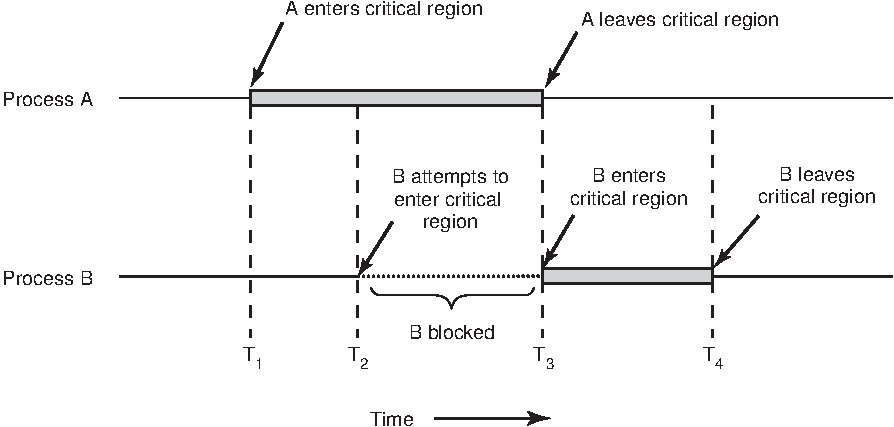
\includegraphics[width=.9\textwidth]{cr}
  \bicaption{临界区域与竞争}{Critical region}
  \label{fig:critical}
\end{figure}

在图~\ref{fig:critical}\cite{tanenbaum2008modern}所示的例子中,
进程A在$T_1$时刻进入了临界区域,片刻之后,在$T_2$时刻进程B也运行到了临界区域,但因为此时已
经有一个进程处于临界区域内了,即进程A,根据互斥法则,进程B将无法成功进入临界区域,此时,进
程B将会被处于等待进程A的临界区域退出中。之后不久,在$T_3$时刻,进程A完成了对临界区域的操作并且
退出,此时,进程B便能立刻进入临界区,最后,进程B在$T_4$时刻也完成了对临界区的操作,此时,系
统回到了没有进程处于临界区内的状态了。

%\subsection{锁机制}\label{sec:lock}

% 实现互斥的方法主要有关中断和锁机制。其中,关中断是要求每个进程在进入临界区域后立即关闭所有
% 的中断,并在进程使用完临界区域后立即打开中断。这一方法实现的原理是:在关闭中断的条件下,进
% 程便可放心对临界区域进行读写操作,而不用担心因时钟中断而引起的进程切换,或者为了运行其它中
% 断处理程序而必须停止对临界区域的操作。屏蔽中断对于只有一个CPU的系统效果是非常明显。进程只要
% 把中断屏蔽了,此时别的进程便无法使用CPU,于是从根本上做到了临界区的互斥访问。并且由于不再需
% 要运行中断处理程序,使得进程能够干净利落地处理完临界区域内的事情从而能快速退出临界区域。但
% 是在多处理器系统里,这种方法却不太实用,因为,进程执行的关中断指令,只对进程所占用的当
% 前CPU发生作用,系统里别的CPU却可以正常接受中断,所以,仍然可能存在来自不同CPU的进程同时进入
% 临界区域的问题。此外,关中断本身是一个权限比较高的指令,如果把这样一个指令完全放手给用户进
% 程来使用的话,就极有可能会出错。一个系统要运行各种来自不同用户的形形色色的程序,只要某一个
% 程序员在自己的程序代码中忘记了在退出临界时恢复中断的话,那么由于整个系统都无法接受任何中断,
% 此时时钟中断不能生效,系统便无法进行进程切换,在当前使用CPU的进程退出或者阻塞后,CPU将闲置
% 着,而别的一大堆着急着运行的进程却无法使用CPU,这时候的系统就相当于完全停止工作了,这中情况
% 显然是相当可怕的。如此看来,关中断虽然看起来简单易行但并不是实现互斥的一个理想的方法。

\subsection{锁机制的实现}
\label{sec:lock}

实现临界区域互斥访问的一个比较常用的有效方法是锁机制。锁机制的原理是,给每一个共享数据
分配一个锁变量,这个锁变量在任意一时刻只能最多被一个进程所持有。任何进程在欲进入临界区域时,
必须先通过检查锁变量的值(值为0表示可用,非0则表示不可用)来判断锁是否可用。如果检查到锁
变量的值为0,则立即把值更新为1(非0值),以排斥其他进程的进入,然后进入临界区域,进程退出
临界区域后便把该变量的值恢复回0;如果检查到锁变量的值为非0,则需等待其他进程把变量设置为
0后方能进入。

上述锁机制存在着一个问题,如果有两个进程恰巧同时检测到锁变量的值为0,于是两个进程
都把该值变为非0,于是这两个进程都进入了临界区,此时又产生了竞争,如程序~\ref{src:race1}所
示。

\begin{listing}[H]
  \begin{codeblock}
\begin{ccode}
acquire(struct lock *lk){
  for(;;){
    if(!lk.locked) {
      lk.locked=1; //这里将出现Race condition
      break;
    }
  }
}
\end{ccode}
  \end{codeblock}
  \bicaption{存在竞争}{Race condition exists}\label{src:race1}
\end{listing}

显然,问题出现的原因是由于进程获取锁这一个事情分成了两个步骤即查看变量值是否等于0和把值变
为0。所以,必须做到把这两个步骤合并为一个步骤,才能断绝出现一个进程正在更新变量的值的时候,
另外一个进程溜了进来并也成功把变量值设置为非0。如何把两个步骤合为一个步骤是通过一条特殊
的CPU指令来实现的,那便是\texttt{xchg}指令。\texttt{xchg}指令实际上就是把两个操作数的值对掉
一下,最后返回旧操作数的值。使用\texttt{xchg}指令后,获取锁的过程便由程序~\ref{src:race1}变
成了程序~\ref{src:race2}。

\begin{listing}[H]
  \begin{codeblock}
\begin{ccode}
acquire(struct lock *lk){
  while(xchg(&lk->locked, 1) != 0);
}
\end{ccode}
  \end{codeblock}
  \bicaption{避免竞争}{Race condition avoided}\label{src:race2}
\end{listing}

在程序~\ref{src:race1}中,如果两个进程同时运行到了第3行,都检测到\texttt{lk.locked==0},于
是都迅速抓住了锁,便执行第4行,就造成了两个CPU都持有锁,这显然是与互斥原则想违背的。在程
序~\ref{src:race2}中,\texttt{xchg}指令首先把\texttt{lk.locked}的值与1进行交换,之后再返
回\texttt{lk.locked}原来的值。如果\texttt{lk.locked}的值为0,那么与1交换就直接相当于把它更
新为1了,然后再返回一个0告知进程已成功获得锁。

% \subsection{锁的使用}

% 锁在处理临界区的问题上,便捷而有效,虽然便捷有效,但也不是处处都要用到。锁用得越多,系统
% 的并行处理能力便会下降。所以,锁并非用得越多越好,而是只在必要的时候才需要用锁。对于如何搞
% 清楚锁的必要性和如何决策该用多少个锁,以及每一个锁又是用来保护哪些数据的这个问题向来是不
% 容易的。这就要求做到,任何时候遇到一个数据如果具有被一个进程正进行写的同时,别的进程也可
% 以对它进行读写的特点的话,那么这个数据就必须得用锁保护起来。另外,锁在使用时,要注意顺序
% 性。因为有些时候,进程可能需要获取多个锁才能进入一个临界区。这种情况下,就要求所有访问这
% 个临界区域的进程都必须按相同的顺序来一一获取这几个锁,否则就有可能造成死锁。

\subsection{死锁}

死锁是指,组内的每个成员都一直处于等待状态,等待别的成员做出诸如发送消息或者释放锁的动作,
以便能继续执行任务\cite{Coulouris12}。死锁现象在那些利用锁来保护共享资源的系统里比较常见,
如在多进程系统、并行计算系统,和分布式系统里\cite{padua11}。举例来说,进程1和进程2都需要获
取两个锁(A和B)才能继续工作。但是,进程1是以先A后B的顺序来获取这两个锁;而进程2却是以
先B后A的顺序来获取这两个锁的。这时候就有可能出现,进程1获得A锁的同时进程2也获得了B锁,接下
来,进程1便因等待B锁而被阻塞,而进程2也因等待A锁而被阻塞。两个进程都在等待对方释放所持有的
资源,但双方却又都拥有对方所缺少的资源,于是谁也不能继续工作,也就无法释放所拥有的资源,只
能无限期地等待下去,这种状态就叫死锁。为了防止出现这种情况,可以规定两个进程都按同一个顺序
一一获取这些锁。防止出现死锁的主要方法还有关中断和禁止进程在持有锁的情况下被阻塞。其中关中
断主要应用于进程持有\texttt{spinlock}的情况下,遇到了中断的到来,此时CPU不得不转入该中断处
理程序运行,但不幸的是该中断处理程序又恰巧需要获取该\texttt{spinlock},于是中断处理程序必须
等待进程释放它,但是该\texttt{spinlock}却无法被进程释放,因为进程必须得等到中断处理程序返回
后才能继续运行,于是死锁就出现了。为防止出现这种死锁,就得在获取\texttt{spinlock}之前先关闭
中断。另外一种情况,如果一个进程在持有锁的情况下被阻塞进入睡眠状态的话,那么别的需要这个锁
的进程将会陷入无限期等待。所以,必须要求进程在进入睡眠等待前释放所持有的锁。

\subsection{锁的种类}

前面已经说过,进程在进入临界区域前必须先成功获得锁后方能对临界区域进行读写操作。如果一个进
程在尝试获取锁的时候发现这个锁已经被别的进程持有了,那么这个进程接下来该怎么做?可以有两种
处理方式:第一种是进程一直不断地尝试获取锁这个动作(即所谓的``忙等'',busy
waiting)\cite{wiki:Busywating},直到持有该锁的进程释放该锁后,拿到锁,才能进入临界区;第二种是一
旦发现锁不可用的情况下,立即自愿放弃CPU而进入睡眠状态,等待别的进程释放该锁后再唤醒它。显
然采取忙等的情况会造成一定的CPU时间的浪费,尤其是锁被持有的时间比较长的话就更加浪费CPU时间
了。然而,事实上,有些临界区域的操作时间事件上非常短,甚至短于进行进程切换所耗费的时间。这
种时候采取忙等的方式来获取锁显然就是比较理想的了。前文所提到过的\texttt{spinlock}就是采取这
种方法获取锁的。第二种处理方式则适合于获取那种需要长时间保持的锁,例如文件系统读写硬盘上的
文件,这时候的硬盘操作需要的时间就比较长了,有时甚至需要持续几秒钟。如果继续用忙等的方式来
获取锁的话,那将会造成大量的资源浪费,所以,应该以第二种方式获取。而且为了提高系统效率,现
代操作系统都规定进程在读写硬盘的时候要让出CPU。这个时候就需要一种进程能长时间持有的锁,甚至
在进程被切换出去后仍能持有该锁并继续完成I/O工作,这种锁就是\texttt{sleeplock}。
\texttt{spinlock}的具体定义的代码如程序~\ref{src:spinlock}所示。 

\begin{listing}
  \begin{codeblock}
\begin{ccode}
struct spinlock {
  uint locked; // 锁变量,值为0表明可用,值非0表示不可用;
  struct cpu *cpu; // 持有该锁的CPU;为方便调试时用;
};
\end{ccode}    
  \end{codeblock}
  \bicaption{\texttt{spinlock}结构体}{\texttt{struct spinlock}}\label{src:spinlock}
\end{listing}

获取\texttt{spinlock}的过程中需要首先关闭中断,以防止进程在持有spinlock的情况下被中断信号打
断从而可能引起的死锁问题。中断将在进程释放\texttt{spinlock}的时候开启。\texttt{acquire()}函
数的代码如程序~\ref{src:acquire}所示。

\begin{listing}%[H]
  \begin{codeblock}
\begin{ccode}
void acquire(struct spinlock *lk) {
  pushcli(); // 首先关中断以避免死锁;
  if(holding(lk))
    panic("acquire");

  while(xchg(&lk->locked, 1) != 0);

  lk->cpu = mycpu();
}
\end{ccode}
  \end{codeblock}
  \bicaption{\texttt{acquire()}函数}{\texttt{acquire()} function}\label{src:acquire}
\end{listing}

\texttt{sleeplock}的定义如程序~\ref{src:sleeplock}所示。

\begin{listing}%[H]
  \begin{codeblock}
\begin{ccode}
struct sleeplock {
  uint locked;        // 锁变量;
  struct spinlock lk; // 用来保护sleeplock,以防出现死锁;
  // 为方便调试:
  char *name;         // 锁的名称;
  int pid;            // 持有锁的进程;
};
\end{ccode}
  \end{codeblock}
  \bicaption{\texttt{sleeplock}结构体}{\texttt{struct sleeplock}}\label{src:sleeplock}
\end{listing}

由于获取\texttt{sleeplock}的过程需要分几步才能完成,只交换两个操作数值的\texttt{xchg}指令无
法完成这一个工作,因此,为了防止两个进程同时获取\texttt{sleeplock}而产生竞争而把获
取\texttt{sleeplock}的过程代码当成是临界区域,用一个\texttt{spinlock}保护起来。所有欲获
取\texttt{sleeplock}的进程必须首先获得\texttt{spinlock}。因此,获取sleeplock的过程主要分为
三步:首先获取属于该\texttt{sleeplock}的\texttt{spinlock},在成功获取\texttt{spinlock}后,
再查看\texttt{sleeplock}是否已经被别的进程占用,如果已经被占用的话,进程则以进入睡眠状态的
方式来等待该\texttt{sleeplock},当然,为了防止出现死锁,进程首先释放已取得
的\texttt{spinlock}后方可进入睡眠状态。如果\texttt{sleeplock}没有被别的进程占用的话,进程则
可通过把\texttt{sleeplock}的锁变量值更新为1并且把\texttt{sleeplock}对应的进程设置为当前进程
的方式来获取锁,最后进程释放\texttt{spinlock}。获取\texttt{sleeplock}的函
数\texttt{acquiresleep()}的具体定义如程序~\ref{src:acquiresleep}所示。

\begin{listing}
  \begin{codeblock}
\begin{ccode}
void
acquiresleep(struct sleeplock *lk)
{
  acquire(&lk->lk);
  while (lk->locked) {
    sleep(lk, &lk->lk);
  }
  lk->locked = 1;
  lk->pid = myproc()->pid;
  release(&lk->lk);
}
\end{ccode}
  \end{codeblock}
  \bicaption{\texttt{acquiresleep()}函数}{\texttt{acquiresleep()} function}\label{src:acquiresleep}
\end{listing}

本文主要围绕进程管理和内存管理进行研究,对文件系统部分涉及较少。所以,此处探讨的重点
是\texttt{spinlock}的使用,而非\texttt{sleeplock}。本文所讨论的\texttt{spinlock}主要用于保
护进程表,即\texttt{ptable}结构体里的\texttt{proc[]}数组,和存放所有打开的文件的列表数组,
即\texttt{ftable}结构体里的\texttt{file[]}数组,还有时钟变量\texttt{ticks}。

以保护\texttt{ptable}的\texttt{spinlock}为例,\texttt{ptable}里的\texttt{proc[]}数组记录的
是系统内所有进程的各种状态信息,每一次进程的创建、运行、切换、终结,都要涉
及\texttt{proc[]}数组内相应的数据的读写。其中,进程在创建时,需要在\texttt{proc[]}数组里找
到一个空的位置,然后把该位置设置为``已占用''。此时的操作必须是互斥的,否则就有可能出现两个
进程几乎同时扫描到同一个空位置,接下来便把它更新为已占用,这样的话,先动手的进程的更新便被
后动手的进程的更新给覆盖了。同样,调度器在运行进程前需要把进程的状态改为\texttt{running}态,
如果在调度器把进程从\texttt{runnable}状态改为\texttt{running}状态的过程中,另外一个CPU的调
度器读到了该进程的状态为\texttt{runnable},于是,它也把该进程加载过去运行,此时就会出现一个
进程同时被两个CPU重复运行的情况。所以,对这样一个所有CPU,所有进程都共用的数据结构,必须要
用一个锁保护起来。由于,进程对\texttt{proc[]}数组的读写都非常简单快捷,所以用一
个\texttt{spinlock}就很合适。\texttt{ptable}的定义,已在第~\pageref{fig:ptable}页给出,这里
不再重复。

\subsection{进程的阻塞与唤醒}

一个进程在系统中存在的状态有四种(\texttt{runnable, running, zombie, sleeping}),但任一时
刻内,一个进程只能以其中一个状态存在。对于前面三种状态已经在前文讨论过了,现在要说
的\texttt{sleeping}态,即阻塞态。阻塞态是指进程需要等待别的进程完成某件事情后方可继续执行。
如等待一个正在被别的进程使用的公共资源的释放或者等待一个子进程的退出或者等待一个I/O操作的完
成等事情\cite{stallings11os}。进程在等待时,与其在不停地主动查看所等待的事情是否已经完成,
空浪费CPU的时间,不如主动进入睡眠状态,让出CPU使用权,在所等待的事情完成后由别的进程以通知
的方式告知该进程,从而避免了忙等(busy waiting)所造成的资源浪费的问题。进入睡眠状态的进程
会被记录在一个睡眠链表中,当别的进程把该进程所等待的事情完成后,便给该链表发送一个信号,以
唤醒该链表内所有在睡眠的进程,此时链表内所有符合条件的进程都由\texttt{sleeping}态转
为\texttt{runnable}态。进程进入通过调用\texttt{sleep()}函数进入阻塞态,并由别的进程调
用\texttt{wakeup()}函数唤醒。\texttt{sleep()}函数基本思想是:把当前进程加入到睡眠队列
(\texttt{chan})内,然后把进程状态标志为\texttt{sleeping}态,最后调用\texttt{sched()}函数
让出CPU。\texttt{wakeup()}函数从指定睡眠链表里把进程唤醒,把进程状态标志
为\texttt{runnable}态。\texttt{sleep()}和\texttt{wakeup()}可以使用任意的数据来区别不同的睡
眠链表,只要\texttt{sleep()}和\texttt{wakeup()}能用同一个数据就成。当然使用跟等待有关的数据
的则更明了。

\texttt{sleep()}的主要工作过程如下。首先确保调用\texttt{sleep()}函数的是当前运行的进程,并
且确保进程已经将所持有的锁(lock)传给\texttt{sleep()}函数了。这主要是进程在调
用\texttt{sleep()}前总是已经持有某个lock。如,\texttt{wait()}在先取得\texttt{ptable.lock}后
才能扫描\texttt{proc[]}数组找一个\texttt{zombie}的子进程为其释放资源,但是如果子进程均没有
运行完毕的话,\texttt{wait()}则需要等待其中一个进程运行终结。此时,\texttt{wait()}便会调
用\texttt{sleep()}并把\texttt{ptable.lock}传给它。这样\texttt{sleep()}函数在更新进程状态的
时候就不需要再次获取该\texttt{ptable.lock}了。如果进程在调用\texttt{sleep()}前持有的锁不
是\texttt{ptable.lock}的话,则需要先获取\texttt{ptable.lock}后再将该\texttt{lock}释放,这样
方可避免出现别的进程在当前进程尚未完成进入\texttt{sleep()}的准备工作之前已经发送了一个唤醒
信号而导致出现该信号被漏掉的\texttt{lost-wakeup}现象。接下来\texttt{sleep()}函数便把当前进
程加入到指定的睡眠链表内并更新其状态为\texttt{sleeping}然后调用\texttt{sched()}让出CPU。之
后进程会一直处于\texttt{sleeping}态直到别的进程给它发送一个唤醒信号,并把它的状态更新
为\texttt{ruannable}态后进程才能重新接受调度,在进程重新运行起来后,\texttt{sleep()}便把进
程从睡眠链表里撤出,并重新获取进程在调用\texttt{sleep()}前所持有
的\texttt{lock}。\texttt{sleep()}函数的具体定义参见参见附录~\ref{sec:sleep}。

\chapter{内存管理的设计与实现}

内存管理从本质上来说就是一种资源管理,只不过在这里所要管理的对象是计算机系统里的内存(RAM)
而已。内存是计算机系统里一个非常重要的资源,所有程序的运行都依赖于内存。虽然随着现代科技的
迅猛发展,内存的尺寸也越做越大,但同时,系统对内存的需求也在飞速增长,而且增长的速度远远大
于内存增长的速度\cite{drepper2007every}。所以,如何在有限的内存空间里同时运行多个进程还一直
是操作系统研发的重点。内存管理是操作系统里专门负责管理内存的一个模块,主要工作就是高效率地
管理这个有限的内存空间,如,给进程分配运行空间、回收进程不再使用的空间、记录已使用的和未使
用的内存区域等一系列事务。

\section{总体设计模型}

内存管理所需完成的工作主要有:如何为用户提供一个内存的抽象,如何管理组织系统内的空闲内存,
如何尽可能地节约内存的分配,以及如何回收内存。本项目的内存管理功能模块如
图~\ref{fig:mem-top}所示。

\begin{figure}[t]
  \centering
  \begin{center}
    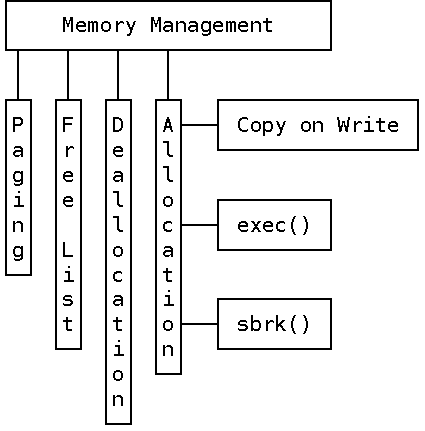
\includegraphics[width=.3\textwidth]{mem-top}
  \end{center}
  \bicaption{内存管理功能模块图}{Memory management modules}
  \label{fig:mem-top}
\end{figure}

%\section{虚拟内存}

% 早期的系统并没有提供内存的抽象,系统工作在``实模式'',每个进程看到的地址都是实地址,即实实
% 在在的物理内存地址。当程序中出现诸如\texttt{mov 100 register1}这样的的指令时,物理内存地址
% 号为\texttt{100}的地方所存放的东西就会被送进\texttt{register1}寄存器内。在这种情况下,如果
% 两个程序中出现相同的地址,那么想要同时运行两个进程就是不可能的。如果其中一个程序要往某个地
% 址里写东西,就会写到别的进程里去了,这时候必然导致系统的崩溃。另外,让物理地址直接暴露给用
% 户进程,会带来很大的安全隐患。如果用户程序可以寻址内存的每一个地址,它们就可轻而易举地破坏
% 操作系统,不管是有意的还是无意的。这些情况的产生都是由于程序中使用了绝对物理地址而造成的,
% 因此为了解决这个问题,必须把物理内存地址对用户程序隐藏起来,而给用户程序呈现一个抽象的
% 内存空间,即虚拟内存。

分页机制是实现虚拟内存一种技术,主要是为用户进程提供一个对内存的抽象,它使得应用程序认为它
拥有连续可用的内存(一个连续完整的地址空间)。而实际上,一个程序所使用的虚拟内存空间通常被
分隔成多个逻辑部分,即所谓的``段''(segment),如代码段、数据段、堆、栈等等。在程序运行时,
这些段会被加载到物理内存中。值得注意的是,程序运行时,操作系统并不需要把该程序完整地加载入
物理内存。如果程序较大的话,通常操作系统只会把该程序中马上要用到的部分加载到物理内存中,也
就是``按需加载''。那些暂时存储在外部磁盘存储器上的部分,会在需要时被加载入物理内
存\cite{Bhat2017}。与没有使用虚拟内存技术的系统相比,使用这种技术使得大型程序的编写变得更容
易,首先程序员不需要担心程序大小是否已经超过物理内存的大小。其次,程序员在操作地址时也不需
要担心这些地址是否会与别的程序使用的地址冲突,因为程序里出现的一切地址都会被系统当成虚拟
(逻辑)地址进一步处理,而不是直接送往地址线上。负责处理逻辑地址的硬件功能模块是``内存管理
单元''(MMU)。MMU是CPU集成电路的一部分。CPU给出的地址(逻辑地址)首先会送往MMU进行地址翻译,
翻译完成后再送往地址线上\cite{abhishek2002memory,Thompson78uniximplementation}。

Freelist是用来管理系统里的所有物理内存空闲页面所创建的一个链表。在给进程分配内存时是每次从该链表
中拿出一页交给进程;回收内存的时候则是把不再使用的页面加入到该链表中。

Allocation 负责的是为进程分配内存,主要通过写时复制的方法来解决进程创建时的内存分配,以及如何
为有需求的进程进行重新映射地址空间和如何处理进程运行时的内存分配。

Deallocation 这一部分实现的是如何为进程回收不再需要的内存资源,包括运行时的内存回收和运行结
束后的内存回收。

\section{详细设计与实现}

内存管理主要是实现如何高效率的分配内存,如何回收内存,以及如何管理空闲内存。这一节将讨论如
何实现这几个功能。

\subsection{分页机制}

虚拟内存概念引入的主要目的是为了防止程序直接访问物理内存和访问不属于自己的地址空间,所以虚
拟内存的主要任务就是实现地址重定向和地址空间的保护。实现虚拟内存的技术主要有:分段技术和分
页技术。

\subsubsection{分段技术}

分段技术出现得比分页技术早。分段技术的基本思想是:将程序所占用的内存分为若干段(segment),
段的大小可以不一样,每个段有一个段号和一个表示段大小的limit\cite{duarte:mem}。如
图~\ref{fig:segmentation}所示,当处理器要进行内存寻址时,所给出的地址就包含了段的号码,以及
段内偏移量(offset)。系统根据地址里提供的段号(段选择子,segment selector)查询段描述符表
(descriptor table)得到该段的基址(base address)再根据地址里所给出的偏移量找到CPU所要求的
地址单元。

\begin{figure}[!ht]
  \centering
  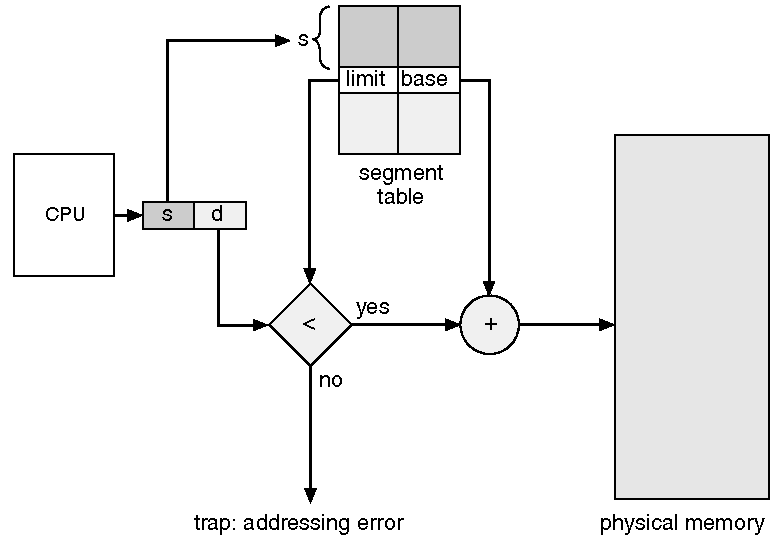
\includegraphics[width=.8\textwidth]{segmentation}
  \bicaption{段式虚拟内存地址翻译过程}{Address translation via segmentation}
  \label{fig:segmentation}
\end{figure}

一个程序通常包含数据段,代码段,BSS段、堆、和栈等若干部分。内核在把程序段加载进物理内存前,
首先得在物理内存内为程序找到空的位置,然后再加载程序段。内核把程序段与所在的物理内存段的对
应关系记录在一张表格中,这张表就叫段描述符表(Segment Descriptor Table)。CPU在每次访问内存
时,内核会首先查询这张表以找到程序的段所在的内存段的入口地址,然后再加上段内偏移量就得出一
个物理地址,送往地址总线\cite{brey2009intel,x86assemblymanual}。如果地址里所给出的段内偏移
量超出了该段的限制的话,系统就会产生一个段错误(segmentation fualt)通知内核,内核便会终止
该进程的运行。

分段技术实现了地址的重定向和地址空间的保护,但却存在一些问题:在系统运行的过程中,由于不断
会有新的进程被加载入内存,同时也不断有进程运行结束,释放内存,而且进程所占用的内存段,既不
连续,大小也不固定,在系统运行一段时间后,物理内存中的剩余空间会呈现``碎片化''现象,即内存
中会产生很多不连续,且大小不等的剩余空间,这就是所谓``外部碎片''。在这种情况下,如果有一
个新进程需要运行,操作系统很可能无法从这些碎片中为其找出一个大小合适的空闲段来加载该进程。
此时如果使用一个较大的段的话也会造成内存空间的浪费。

分页技术出现后,分段技术的使用已经越来越少,许多新推出的处理器甚至不再支持分段机制了。另一
些系统同时支持分段和分页机制,如Intel的奔腾处理器,CPU给出的虚拟地址在送给MMU之后,首先会经
过分段模块的处理,分段模块把虚拟地址翻译成线性地址后,再交给分页模块进行最后的物理地址翻译
(如图~\ref{fig:addr-trans}所示)。

\begin{figure}[!ht]
  \centering
  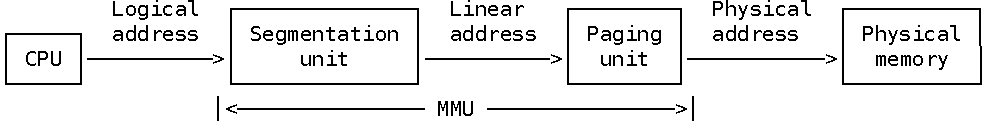
\includegraphics[width=.8\textwidth]{addr-trans}
  \bicaption{Intel奔腾处理器的地址翻译过程}{Intel Pentium virtual address translation}
  \label{fig:addr-trans}
\end{figure}

Linux系统主要依赖于分页技术,而不用分段机制,这一方面是因为分段与分页这两种虚拟内存技术功能
大同小异,采用其中一个就够了;另一方面是因为很多硬件架构都放弃了分段技术。因此,Linux为了达
到跨平台的目的,当然就要最大程度地绕开分段技术。通过把所有的段基址都设置为0,把所有的段限
值(limit)都设置成4G,Linux成功省去了从逻辑地址到线性地址的翻译步
骤\cite{gorman2004understanding}。本实验里采用的就是Linux的这一个处理方法。

\subsubsection{分页技术}

分页技术的基本思想是把程序分成许多个大小相等的块,每一个块称做一页(page),每一页内的地址
都是连续的。相应的,物理内存也被分割成许多个大小相等的块,这些块称做页框(page frame,也叫
物理内存页),页框的大小跟页的大小一致。程序的页会被映射到物理内存中去,每一个虚拟页对应一
个物理的页框,但并非所有的页都要加载进内存才能运行\cite{Sibasankar2010}。描述页与页框之间的映
射关系的表叫做页表(page table),每个进程都有自己独立的页表。在分页机制下,所有CPU给出的地
址都被分成两部分:一个页号(page number)和一个页内偏移量(page offset),如
图~\ref{fig:linear-addr}所示。其中,页号是用来访问页表的下标。页表里给出了所有物理内存页框
的基地址。

\begin{figure}[!ht]
  \centering
  \begin{Large}
    \[%
      \underbrace{%
        \overbrace{00000000000000000010}^{\text{page number (20 bits)}}\,%
        \overbrace{000000000100}^{\text{page offset (12 bits)}}}_{\text{a linear address
          (32 bits)}}%
    \]
  \end{Large}
    \begin{small}
      \[\text{page number}=00000000000000000010=2, \quad \text{page offset}=000000000100=4\]
    \end{small}  
  \bicaption{页号与页内偏移量}{Page number and page offset}
  \label{fig:linear-addr}
\end{figure}

CPU给出的虚拟地址首先被送入MMU中,MMU主要的工作是负责把该地址翻译成物理地址。MMU首先从虚拟
地址中提取出页号并以该页号为下标访问页表,得出该地址所在的物理内存页的起始地址,然后把该起
始地址加上页内偏移量,就得出一个实际物理内存地址,把它送往地址总线,完成了一个虚拟地址的翻
译。图~\ref{fig:paging}简单展示了一个16位线性地址经过分页处理(查询页表)被翻译成一个15位的
物理地址的过程\cite{tanenbaum2008modern}。分页机制通过地址映射,实现了虚拟内存的地址重定向。
每个进程都有属于自己的页表,页表里只映射了属于进程自己内存空间里的地址,进程无法访问不在自
己页表覆盖范围内的地址,由此实现了进程地址空间的保护。

\begin{figure}[!ht]
  \centering
  \begin{center}
    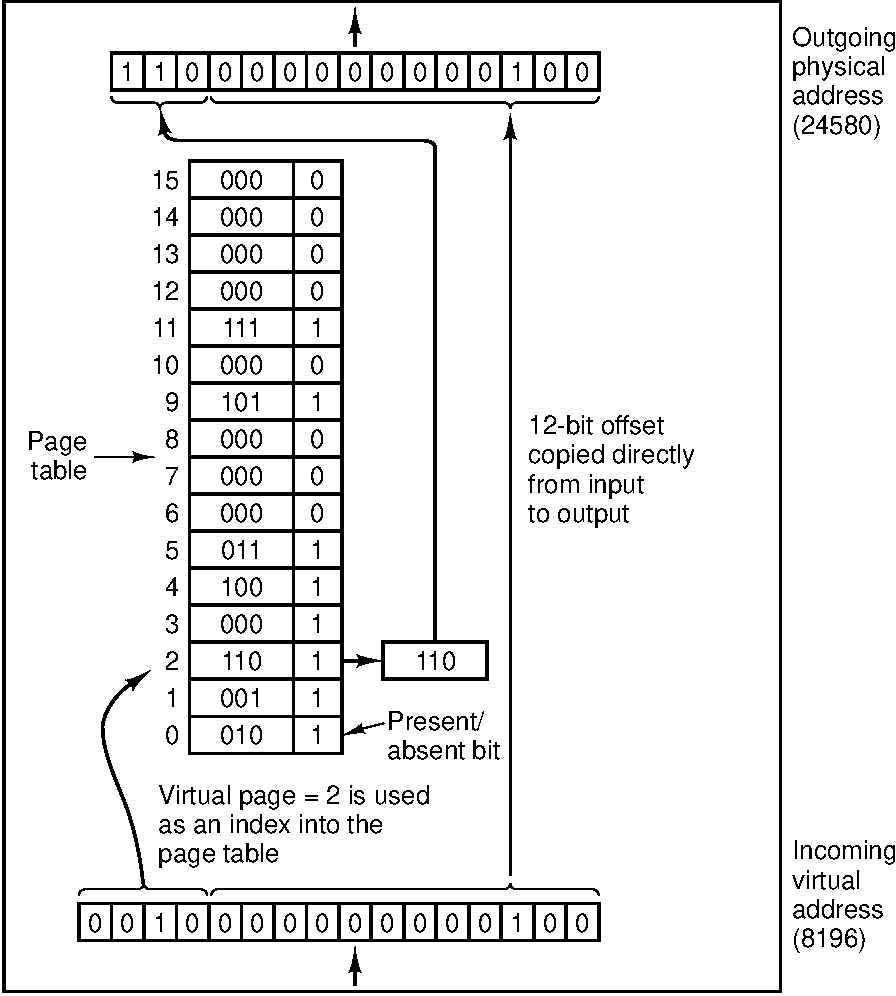
\includegraphics[width=.7\textwidth]{paging}
  \end{center}
  \bicaption{分页地址翻译的过程}{Virtual address translation via paging}
  \label{fig:paging}
\end{figure}

不同的系统对页面的大小的规定不一样,但都是2的n次方,如4kb、8kb、4M等,在32位系统里,采用的
大都是4kb大小的页。由于页是内存分配的最小单位,在分配空间时,如果一个程序的大小没有刚好是页
大小的整数倍的话,那么最后一个页面的空间就没有被完全利用,所浪费的空间就叫``内部碎片''。所
以页面太大的选择就值得考虑。页面越大,内部碎片浪费的空间又会越大;页面越小小,每个程序所需
的页表数量又会越多,页表数量的增加会直接导致加载页表时花费的时间越多,于是最佳页面大小的选
取必须在这几个因素间权衡。Intel奔腾处理器可以支持4K和4M两种大小的页
面,Sun的UltraSPARC支持8K、64K、512K、和4M大小的页面。用户可以根据需要,在编译内核时,选定
某一大小的页面\cite{silberschatz11essentials}。通常,32位系统大多采用4kb大小的页面。

\subsubsection{页表结构}

随着计算机科学技术的发展,现代处理器的寻址空间都达到了32位,甚至64位。在这种情况下,一个程
序的虚拟地址空间可达$2^{32}$或$2^{64}$个字节的大小\cite{zos}。以32位系统为例,如果每个页面
的大小为4k,页表中每条记录(page entry)的宽度为4字节,那么就需要 $2^{32}/4k=1M$ 条记录才能
覆盖4G的虚拟内存空间。于是,一个进程的页表本身就要占用 $1M\times 4 = 4M$ 的内存空间。为了存
放这一个页表,就得在物理内存里找到一块4M大小的连续区域。如果系统内有N个进程,就要消耗
掉 $4M\times{}N$ 大小的空间来专门存储页表,这个开销对系统来说显然是比较沉重的。解决这个问题
的一个有效的方法是对页表本身进行分页:将一个4M大的页表分成1K个4K大小的页表,这1K个页表可以
独立存放于物理内存中。另外,系统再拿出一页来专门记录这1K个页表在物理内存中的具体位置,这一
页就叫一级页表(page directory),另外那1K个页表都是二级页表(page table)。由于大部分程序
都用不到整个4G地址空间,实际上,每个进程都只用到了地址空间内的少数几个集中的页面而已,于是
在页面映射时,内核只需把用到的这些页面映射到物理内存上,而被映射的虚拟地址才需记录在二级页
表内,此时二级页表的数量就可以根据实际需要来定了,如果只有1K个虚拟页需要映射到物理内存,那
么系统只要花费一张二级页表就足够了。这种二级页表的方法无疑为系统节省了不少的开销。

一级页表里有1k条记录(page directory entry,简称PDE),每条PDE指向一个二级页表。对应的二级
页表的记录叫(page table entry,简称PTE)。PDE与PTE的结构相似,都是高20位代表物理内存页的地
址,低12位代表标志位。Intel奔腾处理器所支持的PTE的结构如图~\ref{fig:i386pte}所示。其
中PDE与PTE的不同之处在于D标志位,该位置0则表示是PDE。标志位的定义如程序~\ref{src:pte-flags}所示。

\begin{figure}[!ht]
  \centering
  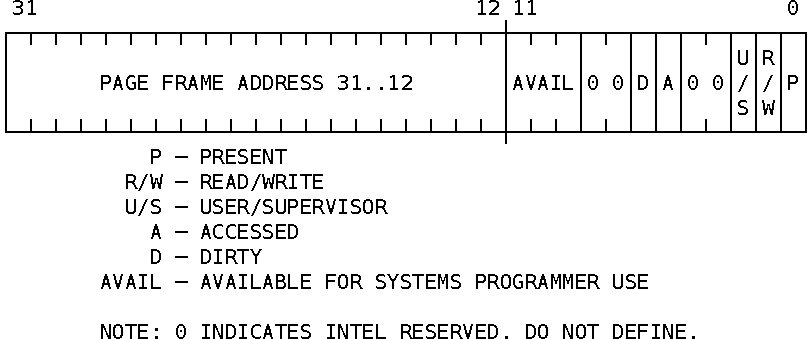
\includegraphics[width=.75\textwidth]{i386pte}
  \bicaption{Intel i386 页表定义}{Intel i386 Page Table Entry}
  \label{fig:i386pte}
\end{figure}

\begin{listing}%[H]
  \begin{codeblock}
\begin{ccode}
#define PTE_P 0x001 //表明该页已经映射
#define PTE_W 0x002 //表明该页可写
#define PTE_U 0x004 //表明该页允许用户访问
#define PTE_A 0x020 //表明该页已经被访问过
#define PTE_D 0x040 //表明该页是二级页表
\end{ccode}
  \end{codeblock}
  \bicaption{PTE标志位}{PTE flags}\label{src:pte-flags}
\end{listing}

在两级分页机制下,CPU给出的虚拟地址被送入MMU,MMU先提取地址的最高10位
(图~\ref{fig:2levelpagingsmall})做为访问一级页表的下标,从一级页表内得出一个二级页表的地
址,再提取接下来的10位地址作为访问该二级页表的下标,并从中得出CPU所要求的物理内存页的开始地
址,然后再加上虚拟地址的最低12位偏移量即可得出一个完整的物理地址,并送往地址总线。两级分页
的地址翻译过程如图~\ref{fig:2levelpaging}所示。

\begin{figure}[!ht]
  \centering
  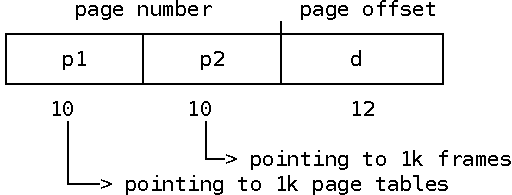
\includegraphics[width=.5\textwidth]{2-level-paging-small}
  \bicaption{32位线性地址两级分页}{Two-level paging virtual address}\label{fig:2levelpagingsmall}
\end{figure}

\begin{figure}[!ht]
  \centering
  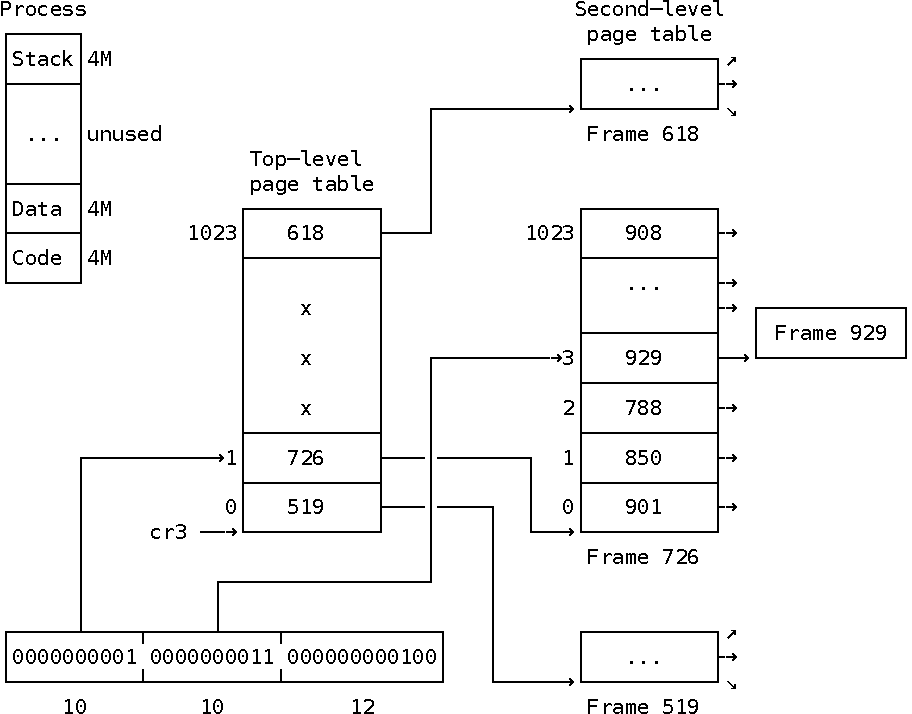
\includegraphics[width=.8\textwidth]{2-level-paging}
  \bicaption{两级分页地址翻译过程}{Two-level paging}
  \label{fig:2levelpaging}
\end{figure}

\subsection{页表的实现}

页表的作用是负责记录虚拟地址到物理地址的映射关系。页表的设置主要完成的工作就是为每一页虚拟
地址找到一个空闲的物理内存页,并把这一个物理内存页的开始地址记录在这个虚拟地址对应的页表项
内,最后再把该页的标志位信息填入页表项内,便完成了一页虚拟地址到一页物理内存地址的映射关系
的填写。本实验把完成页表设置的工作定义在名为\texttt{mappages()}的函数中(附
录~\ref{sec:mappages}),其函数原型如程序~\ref{src:mappages}所示。

\begin{listing}%[H]
  \begin{codeblock}
\begin{ccode}
static int
mappages(pde_t *pgdir, void *va, uint size, uint pa, int perm);
\end{ccode}
  \end{codeblock}
  \bicaption{\texttt{mappages()}函数原型}{\texttt{mappages()} function prototype}\label{src:mappages}
\end{listing}

\texttt{mappages()}函数需要的参数分别是:\texttt{pgdir, va,
  size, pa, perm}。其中,
\begin{itemize}
\item \texttt{pgdir}指向将要设置的一级页表;
\item \texttt{va}指向将要被映射的虚拟地址的开始处;
\item \texttt{size}代表需要映射的总共的虚拟地址大小;
\item 而\texttt{pa}则指向要映射的物理地址的开始处;
\item 最后一个参数\texttt{perm}指定该页是否允许用户访问或是否可写。
\end{itemize}

\texttt{mappages()}函数的工作就是负责把从\texttt{va}开始到\texttt{va+size}的虚拟地址给一页
一页地映射到物理内存的\texttt{pa}开始处,并按\texttt{perm}所指定的值把这每一页的第三个标志
位进行设置。

\texttt{mappages()}函数(附录~\ref{sec:mappages})对二级页表进行设置的详细过程如下:
\begin{enumerate}
\item \texttt{mappages()}函数首先把需要映射的虚拟地址va进行页对齐操作,得到va所在页的
  起始地址a;
\item 然后把a交给\texttt{walkpgdir()}函数(程序~\ref{src:walkpgdir});
\item \texttt{walkpgdir()}函数首先从地址a中取出最高10位作为访问一级页表\texttt{pgdir}的下
  标,从而找相应的\texttt{PDE}所在的单元格,然后检查该单元格是否为空;
  \begin{itemize}
  \item 如果为空,则首先需要分配一个空闲页来作为相应的二级页表,并把新分配到的该二级页表全
    部初始化为0,最后将该二级页表的物理地址填入到单元格的前20位并进行标志位的设置,即可完
    成一条PDE的写入;
  \item 如果该单元内已经存放着PDE,并且\verb|PTE_P|这一标志位为1的话,则表明该条PDE所对应的
    二级页表已经被映射了,此时可直接取出PDE的前20位地址作为找到二级页表的物理地址。
  \end{itemize}
\item 最后再取出a的第12\char`~21位做为下标访问该二级页表,找到相应的PTE所对应的单元格地址
  并将其返回给\texttt{mappages()}函数。
\item \texttt{mappages()}函数检查该单元格内容是否为空,如果为空,则把物理地址pa填入该地址
  的前20位,最后按要求对标志位进行设置,即完成了对二级页表的一条PTE的写入。
\end{enumerate}

\begin{listing}%[H]
  \begin{codeblock}
\begin{ccode}
static pte_t *
walkpgdir(pde_t *pgdir, const void *va, int alloc)
{
  pde_t *pde;
  pte_t *pgtab;
  pde = &pgdir[PDX(va)];
  if(*pde & PTE_P){
    pgtab = (pte_t*)P2V(PTE_ADDR(*pde));
  }
  else {
    if(!alloc || (pgtab = (pte_t*)kalloc()) == 0)
      return 0;
    // 把新分配到的二级页表全部初始为0;
    memset(pgtab, 0, PGSIZE);
    // 其中W和U标志位可在二级页表中进行进一步的设置;
    *pde = V2P(pgtab) | PTE_P | PTE_W | PTE_U;
  }
  return &pgtab[PTX(va)];
}
\end{ccode}
  \end{codeblock}
  \bicaption{\texttt{walkpgdir()}函数}{\texttt{walkpgdir()} function}\label{src:walkpgdir}
\end{listing}

\subsection{freelist的实现}

内核负责为每一个进程分配和回收内存,为了方便对内存的管理,内核把系统里所有的空闲页集中放在
一起,并以链表链表的形式组织起来。内核每次分配内存都是从该链表中拿出一页交给进程;每次回收
一个内存页后,把该页加入链表中。内核把物理内存中从内核结束的地方(\texttt{end})开始
到\texttt{PHYSTOP}的地方(参见图~\ref{fig:va-pa-layout})都用作运行时的内存分配区
域。

存放所有空闲页的链表叫做\texttt{freelist}。\texttt{freelist}里的每一个成员就是一个空闲页。
为了定义一个\texttt{freelist},这里首先对一个空闲页做出了定义。所谓空闲页,就是什么都没有存放的页
面,但是为了能连成一条链表,所有的空闲页都应该有一个指向下一个空闲页的指针。空闲页
(\texttt{run})的定义如程序~\ref{src:run}所示。

\begin{listing}%[H]
  \begin{codeblock}
\begin{ccode}
struct run {
  struct run *next;
};
\end{ccode}    
  \end{codeblock}
  \bicaption{空闲页}{Free page pointer}\label{src:run}
\end{listing}

由于\texttt{freelist}有可能被多个CPU同时访问,所以,必须用一个锁加以保护,
如\texttt{spinlock}。把\texttt{freelist}和\texttt{spinlock}打包,一起放在\texttt{kmem}数据
结构内(程序~\ref{src:kmem})。需要说明的是,系统在初始化时,只启动了一个CPU,其它的CPU尚未
初始化,此时,访问\texttt{freelist}并不需要使用\texttt{lock},所以,在\texttt{kmem}里增加一
个\texttt{use\_lock}变量,就是为了控制是否需要使用锁才能访问\texttt{freelist}。

\begin{listing}%[H]
  \begin{codeblock}
\begin{ccode}
struct {
  struct spinlock lock;
  int use_lock;
  struct run *freelist;
} kmem;
\end{ccode}    
  \end{codeblock}
  \bicaption{\texttt{kmem}结构体}{\texttt{struct kmem}}\label{src:kmem}
\end{listing}

内存分配是以页为单位的,内核每次从\texttt{freelist}链表中取出第一个空闲页交给进程。实现内存分配的函
数是\texttt{kalloc()}函数(程序~\ref{src:kalloc}),其主要工作过程是:
\begin{enumerate}
\item 首先检查\texttt{kmem}里的\texttt{use\_lock}的变量值,
  \begin{itemize}
  \item 如果为0,则表明不需要获得锁即可直接访问\texttt{freelist};
  \item 如果为1,则表明需要先获得\texttt{spinlock}才能访问\texttt{freelist}。
  \end{itemize}
\item 接下来\texttt{kalloc()}函数取出\texttt{freelist}的第一个页
  面,并重新设置\texttt{freelist}指针让其指向该页面的下一个页面;
\item 最后\texttt{kalloc()}函数把该页面返回给进
  程,即完成了一个页面的分配。
\end{enumerate}

\begin{listing}%[H]
  \begin{codeblock}
\begin{ccode}
char* kalloc(void) {
  struct run *r;
  if(kmem.use_lock)
    acquire(&kmem.lock);
  r = kmem.freelist;
  if(r)
    kmem.freelist = r->next;
  if(kmem.use_lock)
    release(&kmem.lock);
  return (char*)r;
}
\end{ccode}
  \end{codeblock}
  \bicaption{\texttt{kalloc()}函数}{\texttt{kalloc()} function}\label{src:kalloc}
\end{listing}

在一个程序不再使用某个页面时,内核便把该页面释放掉。页面释放的处理方式是把不要的内存页面全
部填充为1,然后把该页面加到\texttt{freelist}中。负责释放页面的函数是\texttt{kfree()}(程
序~\ref{src:kfree})。\texttt{kfree(char *v)}把参数\texttt{v}所指向的物理内存页进行释放,主
要工作过程如下:
\begin{enumerate}
\item \texttt{kfree()}函数首先检查地址v是否合法:\texttt{v}不能释放属于内核的页面,也不能释
  放\texttt{PHYSTOP}以上的页面,另外每次释放都是以页为单位的,所以\texttt{v}必须是页面大小的整数倍。
\item 接下来,把该页面的内容全部填充为1,即填入无效内容; 
\item 获取操作\texttt{freelist}的锁;
\item 把地址\texttt{v}指针结构化成\texttt{run};
\item 最后再把该页加到\texttt{freelist}的表头位置;
\item 释放锁;
\end{enumerate}

\begin{listing}
  \begin{codeblock}
\begin{ccode}
void kfree(char *v) {
  struct run *r;
  if((uint)v % PGSIZE || v < end || V2P(v) >= PHYSTOP)
    panic("kfree"); //不能释放内核所占的页,也不能释放外围设备所占的页面
  memset(v, 1, PGSIZE); //把要释放的页面全部填充为1
  if(kmem.use_lock)
    acquire(&kmem.lock);
  r = (struct run*)v;
  r->next = kmem.freelist;
  kmem.freelist = r;
  if(kmem.use_lock)
    release(&kmem.lock);
}
\end{ccode}
  \end{codeblock}
  \bicaption{\texttt{kfree()}函数}{\texttt{kfree()} function}\label{src:kfree}
\end{listing}

\subsection{进程的地址空间}

每个进程都有自己独立的虚拟地址空间,都有自己独立的页表,而内核的地址空间在每一个进程页表里
都有完整的映射,这样做的好处是方便处理系统调用,异常情况和中断。当进程在运行时,如若发生了
这三种情况,此时CPU不需要切换页表,不需要进行上下文的保存和重载,而是直接在当前进程的地址空
间内便可运行系统调用,异常和中断的处理程序。进程的虚拟地址空间与物理内存空间的映射关系如
图~\ref{fig:va-pa-layout}所示。

\begin{figure}[!ht]
  \centering
  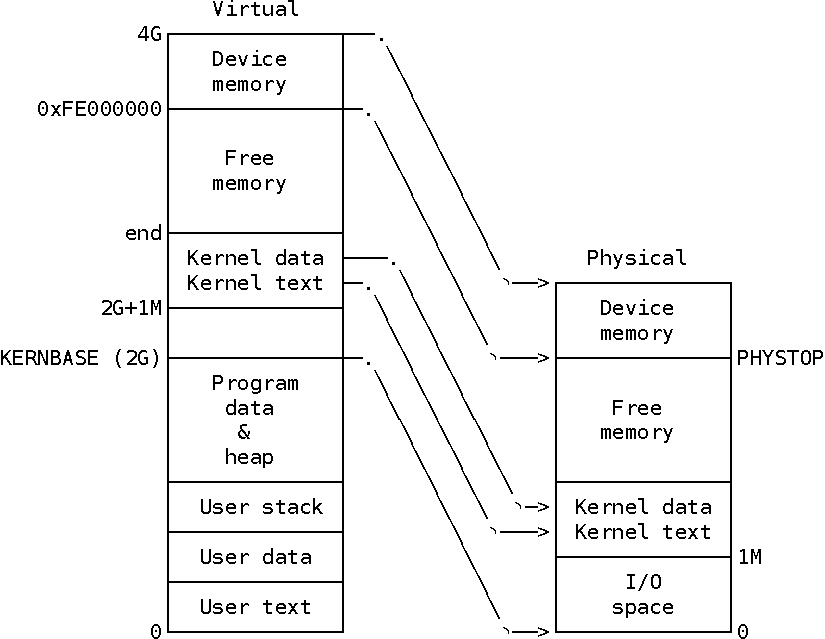
\includegraphics[width=.8\textwidth]{va-pa-layout}
  \bicaption{进程的虚拟地址空间与物理内存的映射关系}{The mapping of virtual address space
    and Physical address space}
  \label{fig:va-pa-layout}
\end{figure}

进程在加载时,内核首先给进程分配一个物理页用于存放一级页表。然后内核再把自己映射到这个页表中。
负责把内核映射到每个进程空间中去的函数是\texttt{setupkvm()}(程序~\ref{src:setupkvm})。

\begin{listing}%[H]
  \begin{codeblock}
\begin{ccode}
pde_t* setupkvm(void) {
  pde_t *pgdir;
  struct kmap *k;

  if((pgdir = (pde_t*)kalloc()) == 0)
    return 0;
  memset(pgdir, 0, PGSIZE);
  if (P2V(PHYSTOP) > (void*)DEVSPACE)
    panic("PHYSTOP too high");
  for(k = kmap; k < &kmap[NELEM(kmap)]; k++)
    if(mappages(pgdir, k->virt, k->phys_end - k->phys_start, (uint)k->phys_start, k->perm) < 0)    
    {    
      freevm(pgdir);
      return 0;
    }
  return pgdir;
}
\end{ccode}
  \end{codeblock}
  \bicaption{内核在进程地址空间内的映射}{The mapping of kernel address space in a process}\label{src:setupkvm}
\end{listing}

其中\texttt{kmap[]}数组(程序~\ref{src:kmap})里规定了内核的各个部分分别被映射到了物理内存
的哪个位置。内核的虚拟地址与物理地址的映射关系如下:
\begin{itemize}
\item 把从\texttt{KERNBASE}开始到\texttt{0x100000}即\texttt{EXTMEM}(\texttt{KERNLINK})的
  这一段虚拟地址映射到从0开始到\texttt{EXTMEM}的这一个物理段,用以做普通I/O设备的存储空间;
\item 把从\texttt{KERNBASE+0x100000}开始到\texttt{data}这一段虚拟地址映射到
  从\texttt{0x100000}到\texttt{V2P}(\texttt{data})的这一个物理段,用来存放内核的代码段和
  只读数据段;
\item 把从\texttt{data}开始到\texttt{PHYSTOP}这一段的虚拟地址映射到
  从\texttt{V2P}(\texttt{data})开始到\texttt{PHYSTOP}的这一个物理段,用来存放内核的可读可
  写的数据段,同时也用作内核的扩张;
\item 把虚拟内存的最高16M直接映射到物理内存的最高16M的地方,用作DMA供显卡、网卡等设备的使
  用。
\end{itemize}

\begin{listing}%[H]
  \begin{codeblock}
\begin{ccode}
static struct kmap {
  void *virt;
  uint phys_start;
  uint phys_end;
  int perm;
}

kmap[] = {
  {(void*)KERNBASE, 0, EXTMEM, PTE_W}, // 映射普通I/O
  {(void*)KERNLINK, V2P(KERNLINK), V2P(data), 0}, // 映射内核的代码段和只读数据
  {(void*)data, V2P(data), PHYSTOP, PTE_W}, // 映射内核的可写数据段
  {(void*)DEVSPACE, DEVSPACE, 0, PTE_W}, // DMA
};
\end{ccode}
  \end{codeblock}
  \bicaption{内核空间地址映射}{Kernel address space mapping }\label{src:kmap}
\end{listing}

\texttt{setupkvm()}函数(程序~\ref{src:setupkvm})的工作过程主要是:
\begin{enumerate}
\item \texttt{setupkvm()}首先调用\texttt{kalloc()}函数为进程分配得一个物理内存页,以作一级
  页表用;
\item 其次把这个新分配到的页表全部初始化为0;
\item 接下来确保\texttt{PHYSTOP}地址要小于\texttt{DEVSPACE};
\item 然后\texttt{setupkvm()}调用\texttt{mappages()},\texttt{mappages()}则按
  照\texttt{kmap[]}数组所定义的顺序把内核所有的部分映射到页表中。
\end{enumerate}

\subsection{虚拟内存的实现}

前面(第~\ref{sec:procvm}节)已经讨论过,每个用户进程的地址空间都包含两部分:内核空间和用户
空间。在上一节里已经讨论了如何实现把物理内存中的内核映射到每个进程的页表中。接下来将讨论如
何实现进程用户空间的内存分配。在给进程分配用户空间时,最直接的办法就是,程序有多大就给它分
配多大的空间,但这样做的后果就是,内存空间会消耗得很快,可能没加载几个进程,内存空间就已经
耗尽了。在程序大小的膨胀速度远远大于物理内存的增长速度的今天这种方法显然不具备很好的实用性。
所以,现代操作系统都通过虚拟内存的技术来实现如何在有限的内存空间内多容纳几个用户进程。实现
虚拟内存的技术主要有:按需加载(demand paging)技术和写时复制(copy-on-write)技
术\cite{silberschatz11essentials}。由于实验时间和资源有限,本实验只选择实验性地实现了其中一
项技术:copy-on-write技术。

\subsubsection{copy-on-write}

copy-on-write(简称COW, 写时复制),是指在创建新进程时,并没有立即为新进程分配物理内存
页,而是让母进程和各个子进程共享(只读)一份物理内存空间,直到其中一个进程(子进程或母进程)
发生了对某个共享页面进行``写''操作时,才给该进程分配一个新的物理内存页,并把要进行``写''操
作的这一个页面的内容从母进程那拷贝一份过来交给子进程。这种只复制要改变的页面的方法相比让每
个新创建的子进程都复制母进程一整份的地址空间的方法要节省很多的物理内存。

COW技术主要用在创建子进程时,为子进程分配物理内存页面的过程中。一般来说,进程在创建以后并不会
立即产生``写''操作,也不会立即运行一份新的程序代码,所以,没必要在创建新进程的时候就立刻就把程序
全部加载到内存。COW的做法是把母进程的页面标志为只读页面,并记录每个页面的被引用次数,母进程
与所有的子进程共享这些只读页面。当母进程或子进程要对这些共享页面中的某一个页进行``写''操作时,内
核首先检查该页面的被引用次数,如果次数等于1的话,则直接把该页面的权限从只读改为可写;如果次
数大于1的话,则表明有多个进程正在共享这个页面,这时候内核将在内存里为该进程申请一个空闲物理
页面,用来复制这个共享页面的内容,并把这个新的物理页面加到该进程的页表中去,然后把该页面的
权限改成可写,最后把共享页面的被引用次数减去1。概括来讲,实现COW技术所需完成的核心工作大致
如下:
\begin{enumerate}
\item 记录每个共享页面的被引用次数;
\item 实现一个\texttt{copyuvm()}函数,负责把母进程的物理页面映射到子进程的页表中,并把这些
  页面标志为只读权限;
\item 处理进程发起``写''操作时的页错误(page fault)异常;
\item 每次更新页表后,重新加载页表寄存器。
\end{enumerate}

\paragraph{首先,记录每个共享页面的被引用次数}

给每个页面增加一个用于记录被引用次数的变量\texttt{pg\_ref},并设计两个函
数\texttt{pg\_refInc()}(程序~\ref{src:pgrefInc})和\texttt{pg\_refDec()},分别用于增、减页
面的被引用次数。当一个物理页面被分配时,把相对应的\texttt{pg\_ref}变量的初值设为1,每当有一
个子进程引用这个页面时,\texttt{pg\_ref}的值加1。相应地,每当有一个进程复制了这个页面
时,\texttt{pg\_ref}的值减1,当\texttt{pg\_ref}的值减到0的时候,这个页面将会被回收。
在\texttt{kmem}结构体里增加一个数组\texttt{pg\_ref[]}用于记录每个页面的被引用次数,如程
序~\ref{src:kmem2}所示。

\begin{listing}%[H]
  \begin{codeblock}
\begin{ccode}
struct {
  struct spinlock lock;
  int use_lock;
  struct run *freelist;
  struct pg_ref[PHYSTOP >> PGSHIF];
} kmem;
\end{ccode}
  \end{codeblock}
  \bicaption{带有\texttt{pg\_ref[]}数组的\texttt{kmem}结构体}{\texttt{struct kmem} with
    \texttt{pg\_ref[]} in it}\label{src:kmem2}
\end{listing}

内核每次给新创建的子进程初始化页表时,实际上都是把母进程所映射的物理页重复映射到该子进程的
页表中,然后调用\texttt{pg\_refInc()}函数把每个物理页面的被引用次数都增加1。当内核需要为某
个进程复制一个共享物理页时,便调用\texttt{pg\_refDec()}函数把该物理页面的被引用次数
减1。\texttt{pg\_refInc()}函数的具体定义如程序~\ref{src:pgrefInc}所示。
\texttt{pg\_refDec()}函数与\texttt{pg\_refInc()}函数大同小异,区别仅在于加1和减1这个操作上,
这里不再单独给出\texttt{pg\_refDec()}函数的具体实现过程。

\begin{listing}%[H]
  \begin{codeblock}
\begin{ccode}
void pg_refInc(uint pa) {
  if(pa<(uint)V2P(end) || pa>=PHYSTOP)
    panic("pg_refInc");
  acquire(&kmem.lock);
  ++kmem.pg_ref[pa >> PGSHIT];
  release(kmem.lock);
}
\end{ccode}
  \end{codeblock}
  \bicaption{\texttt{pg\_refInc()}函数}{\texttt{pg\_refInc()} function}\label{src:pgrefInc}
\end{listing}


\paragraph{其次,实现一个支持COW的\texttt{copyuvm()}函数}

在COW技术中,内核为新创建的子进程的页表做地址空间映射时,实际上是通过遍历母进程的页表,找到
母进程所映射的每一个物理内存页,并把其中具有可写权限的页面统统都改成只读权限外加一个COW的标
志,然后再把这些更改过权限的页面一页一页地映射到子进程的页表中去,完成对子进程的地址空间的
映射。负责为子进程做地址空间映射的这项工作是由\texttt{copyuvm(*pgdir, sz)}函数(附
录~\ref{sec:copyuvm})完成的,其中,参数\texttt{pgdir}代表母进程的一级页表,\texttt{sz}代表
母进程的虚拟地址空间大小。函数负责从\texttt{pgdir}中查出虚拟地址\texttt{0\char`~sz}所映射的
每个物理内存页并把这些物理内存映射到子进程的页表中。\texttt{copyuvm()}的主要的工作过程则如
下:
\begin{enumerate}
\item 首先为子进程分配页表并把内核映射到页表中去;
\item 遍历母进程的页表,查出母进程的所有虚拟地址对应的每一个物理页面; 
\item 检查母进程的每一个物理页面的标志位,如果是可写标志,则改成只读和COW标志;
\item 复制母进程的每一个物理页面的开始地址pa和标志位信息flags;
\item 把复制到的pa和flags映射到子进程的页表中;
\item 把每个物理页面的被引用次数增加1;
\item 最后重新加载母进程的页表寄存器。
\end{enumerate}

\paragraph{最后,实现一个处理页错误的异常处理程序}

由于共享页面被标志成了只读模式,当母进程或者子进程企图对共享页面进行``写''操作时,系统就会
触发一个页错误(page fault)异常。内核对这样的异常情况的处理是:从cr2寄存器里取出页错误的虚
拟地址并检查该虚拟地址是否合法,如果不合法,这个进程会被直接杀死。如果地址合法,则检查该虚
拟地址所对应的物理页面的被引用次数是否大于1,如果大于1,则把该物理页面复制到该进程自己的页表
中并将其更改成可写权限;如果被引用次数等于1的话,则可直接将该物理页面的读写权限改成可写权限
即可。本实验实现页错误异常处理的函数是\texttt{pagefault()}(附录~\ref{sec:page-fault})。
\texttt{pagefault()}函数对页错误的处理过程如下:
\begin{enumerate}
\item 首先从cr2寄存器里读取出错的虚拟地址;
\item 其次,检查对这个地址的访问是否合法,如果不合法,进程会被直接杀死;
\item 查询进程的页表,找到需要进行写操作的共享物理页的地址;
\item 查看该物理的被引用次数:如果被引用次数为1的话,则直接把该页面的权限改成可写权限。如果
  大于1,则为进程分配一个新的物理页。
\item 把共享物理页的内容拷贝到新的物理页中去。
\item 把新的物理页映射到进程的页表中,并把该页面的权限设置为可写;
\item 将原来的共享页的被引用次数减1;
\item 重新加载页表寄存器。
\end{enumerate}

\subsection{测试COW}

现在已经完成了对COW功能的设计与实现,为了验证该技术是否生效,本实验采用一个简单的用户程
序\texttt{testCOW.c}(附录~\ref{src:testCOW.c})来做个测试。该程序所做的事情主要是:调
用\texttt{fork()}系统调用来创建子进程,并调用\texttt{getfreepages()}系统调用来输出系统内的
空闲页的数目,以此观察这些空闲页面的数目在\texttt{fork()}前后的变化和某个进程发生写操作前后
的变化。\texttt{testCOW.c}程序里分别定义了两个小函数\texttt{test1()}和\texttt{test2()}。其
中\texttt{test1()}的功能是查看在母进程没有退出情况下,子进程发生写操作前和后的空闲页面的数
目变化;\texttt{test2()}的功能是查看在母进程退出后,子进程发生写操作的前和后,系统内的空闲
页面数目的变化。输出结果如图~\ref{fig:testcow}所示。

\begin{figure}[!ht]
  \centering
  \fbox{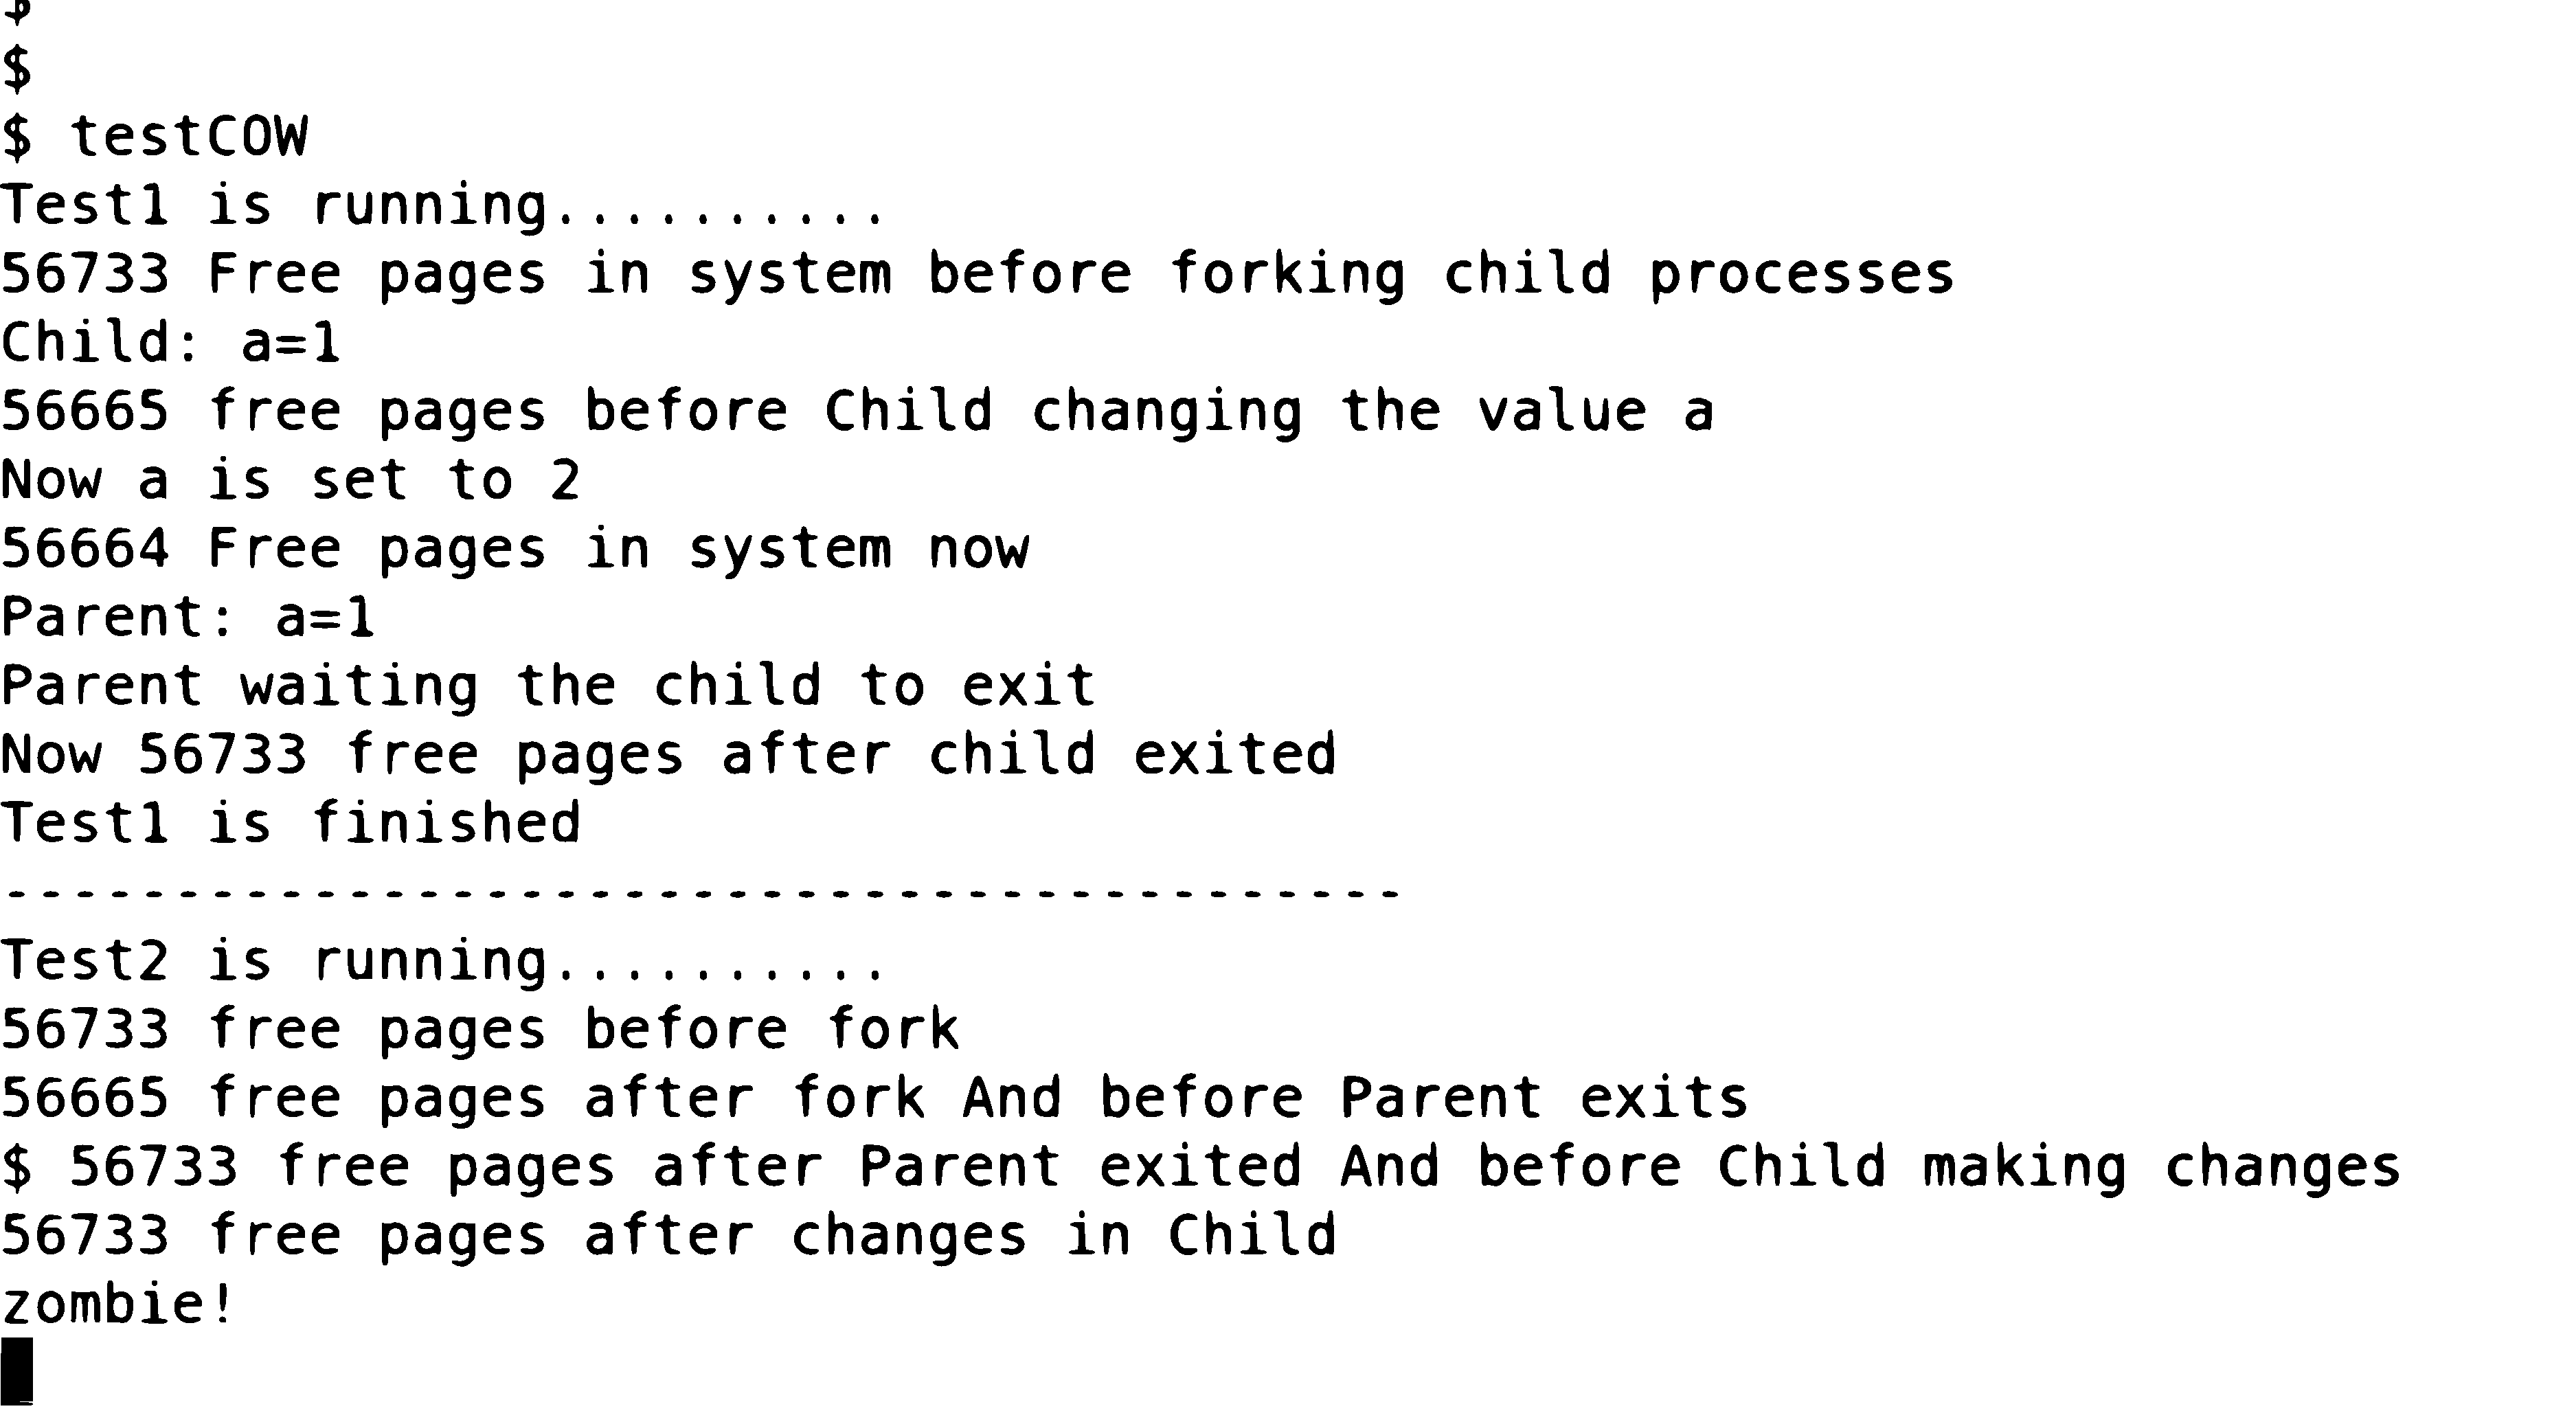
\includegraphics[width=.9\textwidth]{testcow}}
  \bicaption{CoW测试结果输出}{CoW test result}
  \label{fig:testcow}
\end{figure}

\subsubsection{输出结果分析}

\paragraph{\texttt{test1()}输出结果分析}

从图~\ref{fig:testcow}可看出,在创建子进程后,空闲页的数目由56733变成了56665。在子进程改变
了变量a的值后(发生了写操作),空闲页的数目由56665变成了56664,即只减少了一个页。由此可看出,
此时内存的开销只增加了一个页,即4kB。而$56733-56665=68$,这些个页面是用来存放子进程的页表,
同时这个数目也是母进程的页表所占的数目。最后,在子进程退出后,系统里的空闲页数目又变回
了$56664+68+1=56733$。

\paragraph{\texttt{test2()}输出结果分析}

从图~\ref{fig:testcow}可看出,在创建子进程后,空闲页的数目有56733变成了56665。之后,母进程并没
有等待子进程的运行结束,而是自己先退出了。此时,母进程释放了自己的页表所占用的空间,但其所映
射的物理内存页并没有被释放,因为子进程还需使用。此时空闲页的数目变回了$56665+68=56733$。子进
程在母进程退出后,更改了变量a的值(即发生了写),此时由于a所在的物理页面的被引用次数只
剩1(只有子进程在使用)而已了,所以,系统并没有给子进程再分配一张新的物理页而是让子进程直接
在共享页面内进行写操作,所以,系统里的空闲页面并没有减少1,仍然是567333。

综上所述,如果没有实现COW技术,所有的子进程都复制一份母进程的地址空间的话,创建一个子进程,
系统的开销将增加$(68-1)\times{}1k - 1\times{}n$个物理页面。其中,$n$代表进程所需更改的页面个数。

\subsection{\texttt{exec()}}

上一节介绍了如何使用COW技术让所有的子进程和母进程共享物理内存空间。但是,如果一个子进程在
创建运行起来后发现自己要完成的使命跟母进程其实没有多大的联系,即跟母进程并没有存在
合作关系,也不需要共享母进程的代码,而是要运行一份跟母进程
不相关的程序代码,这时候进程就需要有自己独立的一份运行空间。内核为进程提供了这个服务,进程在创
建完毕后,可以通过调用\texttt{exec()}系统调用来重新设置一份完全独立与母进程的运行空间并运行自己的
代码文件。用户进程同过调用\texttt{exec()}系统调用来告知内核它需要一个新的运行空间来运行某个程序代码,
内核接收到这个系统调用后则通过\texttt{exec()}函数来实现为进程重新分配运行空间并加载进程所要求的程
序代码。概括地来说,\texttt{exec()}函数主要完成的工作内容如下:

\begin{enumerate}
\item 检查所要加载程序文件的ELF格式是否正确;
\item 重新为进程分配页表,并重新映射内核到新页表内;
\item 检查ELF文件里的每个程序段的大小信息是否合法以及该程序段是否属于可执行程序段;
\item 检查程序段的大小是否存在溢出的可能;
\item 为每个程序段分配内存空间;
\item 把每个程序段加载进内存空间;
\item 分配新程序用户栈;
\item 将进程指向新的页表;
\item 设置\texttt{exec()}的返回地址为程序代码的入口地址;
\item 释放旧页表所占用的空间;
\end{enumerate}
其中,为进程重新分配新的页表和用户运行空间以及如何加载进程的程序代码是\texttt{exec()}函数工
作的核心。程序~\ref{src:exec}是\texttt{exec()}函数的部分节选,给出了实现这些功能的主要细节。
完整的\texttt{exec()}实现参见附录~\ref{sec:exec}。

\begin{listing}
  \begin{codeblock}
\begin{ccode}
  struct proghdr ph;
  pgdir = setupkvm() //分配页表,并映射内核

  // 读入program headers
  sz = 0;
  for(i=0, off=elf.phoff; i<elf.phnum; i++, off+=sizeof(ph)){
    if(readi(ip, (char*)&ph, off, sizeof(ph)) != sizeof(ph)) //从inode里读入一个proghdr到ph指向的缓冲区内
      goto bad;
      if(ph.vaddr + ph.memsz < ph.vaddr) //防止溢出
      goto bad;
    if((sz = allocuvm(pgdir, sz, ph.vaddr + ph.memsz)) == 0) //为该程序段分配地址空间
      goto bad;
    if(ph.vaddr % PGSIZE != 0)
      goto bad;
    if(loaduvm(pgdir, (char*)ph.vaddr, ip, ph.off, ph.filesz) < 0) //把程序段加载到刚分配得的内存空间中去
      goto bad;
  }
\end{ccode}
  \end{codeblock}
  \bicaption{\texttt{exec()}工作过程(代码节选)}{\texttt{exec()} process}\label{src:exec}
\end{listing}

\texttt{exec()}函数首先调用\texttt{setupkvm()}函数(程序~\ref{src:setupkvm})为进程分配得新
的页表并且完成把内核映射到其中的工作。接下来,\texttt{exec()}函数把可执行文件里的程序段一个
一个地读取到缓冲区内,并检查每个段的长度值和地址范围是否合法。如果合法,则调
用\texttt{allocuvm()}函数(附录~\ref{sec:allocuvm})来为该段分配内存空
间。\texttt{allocuvm()}函数负责以页为单位来为该程序段分配所需的空闲页,并把这些空闲页映射到
进程的新页表中。最后\texttt{exec()}调用\texttt{loaduvm()}函数(附录~\ref{sec:loaduvm})把该
程序段加载到已分配的内存空间中去。其中,\texttt{readi(inode, dst, off, sz)}函数是
从\texttt{inode}指向的文件里的\texttt{off}的开始处读取\texttt{sz}个字节到\texttt{dst}指定的
地方。由于本实验研究的内容是进程管理和内存管理这两个部分,而\texttt{readi()}函数则是属于文
件系统方面的内容,所以本实验只是讨论如何使用这个函数,并没有给出其具体的代码实现。

\subsection{延迟分配(lazy allocation)}

进程的地址空间里有一块叫堆(heap)的区域,这个区域是供进程在运行的过程进行内存申请或释放使
用的。进程在运行的,如果发现内存不够用,需要更多的内存的话或者需要释放某些不需要再使用的页
面的时候,则可通过\texttt{sbrk()}系统调用来告知内核,自己需要增加多少的空间或缩减多少个字节
的空间,内核接收到这个系统调用后则通过调用\texttt{growproc()}函数来为进程分配相应的空间。然
而,有些时候程序里会出现申请一大块的内存空间,然而,这些空间在进程后来的运行中却很少被使用
或者甚至根本不被用到,例如一个程序申请了一个很大的稀疏数组,数组里只有少量的几个值,其余的
空间全部是空或零。这时候,如果也如约地给进程分配一个的数组空间的话,则会造成这其中大部分的
空间被白白的浪费掉。为了解决这个问题,本实验采取了延迟分配(lazy allocation)的方法,即当遇
到进程申请内存空间时,并没有立即给它分配任何的空间,而是采取页错误的处理方法,即当进程真正
需要对这个区域进行操作时,便会促发一个页错误,此后内核在处理这个页错误的时候才会真正在物理
内存里找一个空闲页交给进程。内核对进程的\texttt{sbrk()}系统调用的处理过程大致是:
\begin{itemize}
\item 首先调用\texttt{growproc()}内核函数,检查进程的请求是申请内存还是释放内存;
\item 如果是释放内存,则调用直接调用deallocuvm()函数来释放内存;
\item 如果进程的请求是申请内存的话,则通过把进程的虚拟地址空间增加相应的字节的方法来假装已
  经给进程分配了空间,而实际上并没有。
\item 如果在后期,进程确实发生了对所申请区域的操作,则会促发一个页错误;
\item 内核接收到这个页错误,为进程分配空间。
\end{itemize}
其中,\texttt{growproc(int n)}函数的工作主要是通过检查参数$n$的值来判断进程是需要申请空间
还是释放空间。如果$n>0$,则表明进程需要申请$n$个字节的空间,如果$n<0$,则表明进程需要释放$n$
个字节的空间。\texttt{growproc()}函数的具体定义如程序~\ref{src:growproc}所示。

\begin{listing}
  \begin{codeblock}
\begin{ccode}
int growproc(int n)
{
  uint sz;
  struct proc *curproc = myproc();
  sz = curproc->sz;
  if(n > 0){ 
    sz +=n;//假装给进程分配了空间,实际上只是增加了其虚拟地址空间而已;
   } else if(n < 0){
    if((sz = deallocuvm(curproc->pgdir, sz, sz + n)) == 0)
      return -1;
  }
  curproc->sz = sz;
  return 0;
}
\end{ccode}
  \end{codeblock}
  \bicaption{\texttt{growproc()}函数}{\texttt{growproc()} function}\label{src:growproc}
\end{listing}

\texttt{deallocuvm()}函数(附录~\ref{sec:deallocuvm})主要是负责释放进程
从\texttt{newsz}到\texttt{oldsz}这一段不再需要的内存空间。\texttt{deallocuvm(pde\_t
  *pgdir, uint oldsz, uint newsz)}函数的工作过程比较简单:首先检查\texttt{newsz}的值是否大
于\texttt{oldsz}的值,如果大于,则直接将\texttt{newsz}返回给程序。否则,取
出\texttt{newsz}所在的虚拟页的开始地址,并从页表里找出从该虚拟地址开始往上直
到\texttt{oldsz}结束的这一段的虚拟地址所对应的每一页物理地址。然后再调用\texttt{kfree()}函
数(程序~\ref{src:kfree})将这些物理页面一页一页地释放,最后把\texttt{newsz}返回给程
序。\texttt{kfree()}函数的定义在前文已经给出了,这里不再重复。

内核对由于延迟分配所产生的页错误的处理方法是现时为进程分配所缺物理的页面,并把该物理页面映
射到进程的页表中,完成后便重新加载页表寄存器。为了实现这一个功能,需要
在\texttt{pagefault()}函数里增加一段为进程分配页面并把分配到的页面映射入进程的地址空间中去
的代码,最后,由于进程的页表发生了变化,需要重新加载页表寄存器的值,如程
序~\ref{src:pagefault}所示。 

\begin{listing}
  \begin{codeblock}
\begin{ccode}
pagefault()
 {//延迟分配;
   uint va;
   va=PGROUNDDOWN(cr2());
   char *mem;
   if((mem = kalloc()) == 0) {
     cprintf("kalloc out of memory, kill proc %s with pid %d\n", proc->name, proc->pid);
     proc->killed = 1;
     return;
   }
   memset(mem, 0, PGSIZE);
   mappages(proc->pgdir, (char *)va, PGSIZE, V2P(mem), PTE_W | PTE_U);
   lcr3(V2P(proc->pgdir));
  }
\end{ccode}
  \end{codeblock}
  \bicaption{\texttt{pagefault()}函数}{\texttt{pagefault()} function}\label{src:pagefault}
\end{listing}
 
为了测试刚刚实现的延迟分配方案是否正确发挥了作用,这里写了个简单的用户程
序\texttt{lazyalloc.c}(程序~\ref{sec:lazyalloc})进行测试。该程序的主要工作方式是调
用\texttt{sbrk()}系统调用向内核申请空间或释放空间,内核接收到请求后进行相应的处理。程序通过
观察在调用\texttt{sbrk()}函数之前和之后系统里剩余的空闲页面的变化来判断延迟分配这一个方案是
否正常发挥作用。 \texttt{lazyalloc.c}程序的输出结果图如图~\ref{fig:lazyalloc}所示。
 
\begin{figure}
  \centering \fbox{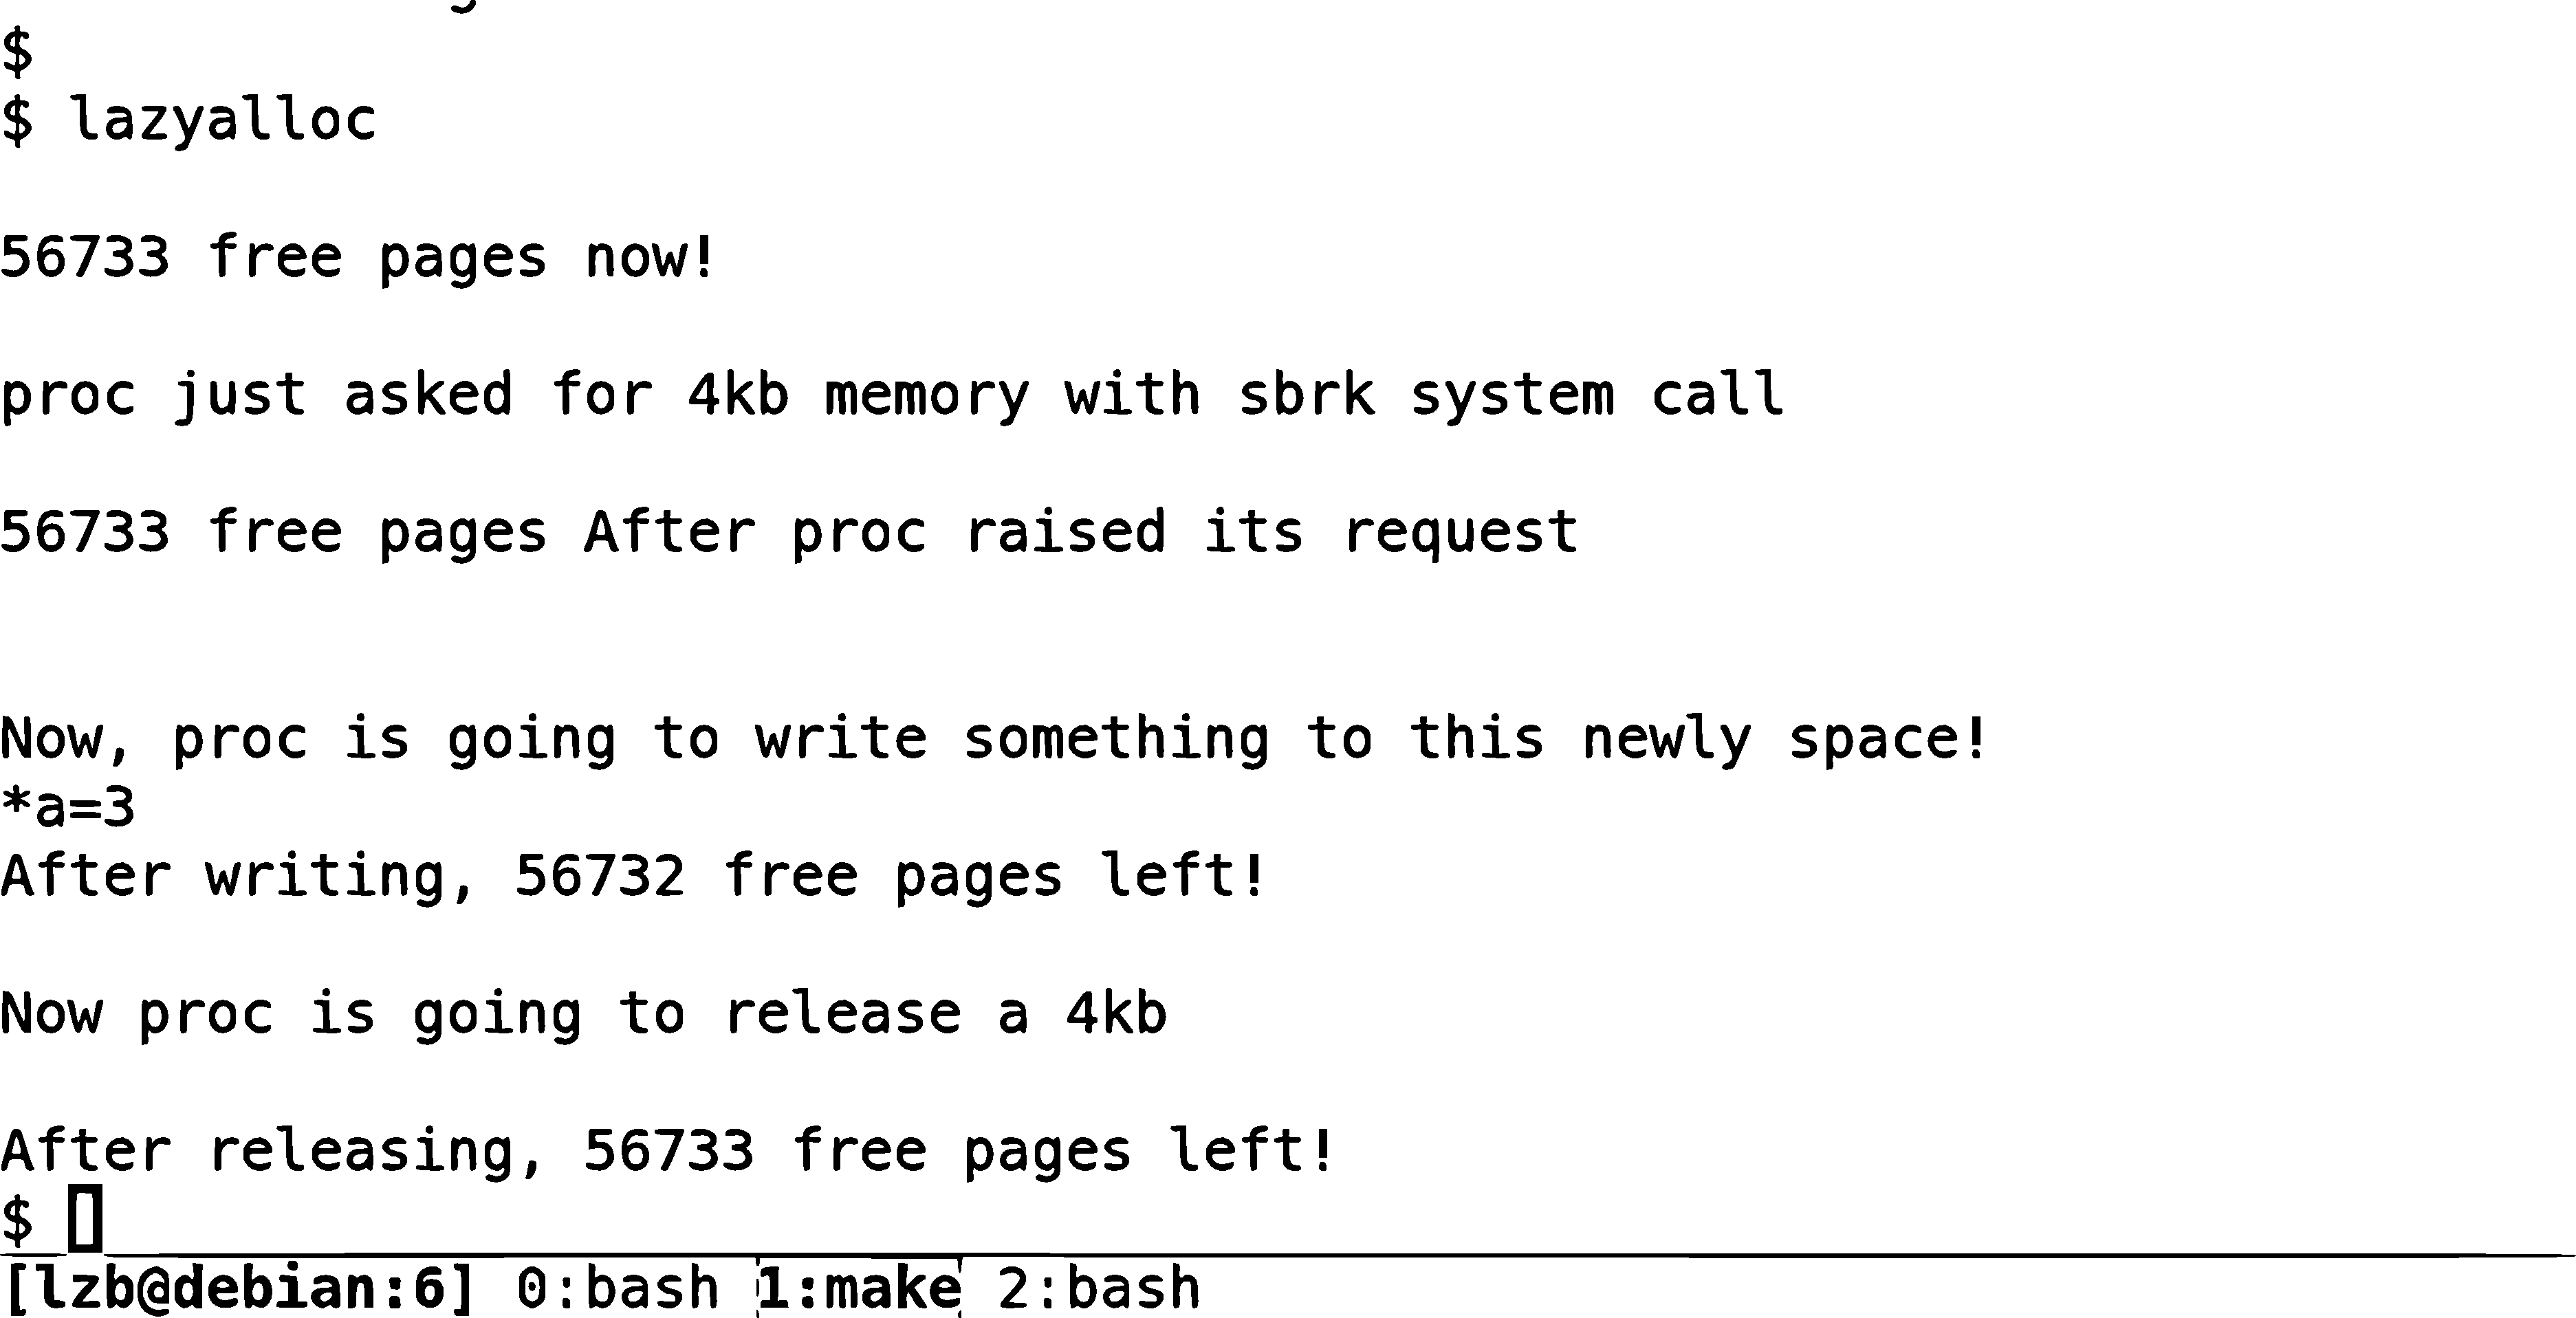
\includegraphics[width=.9\textwidth]{testlazy}}
  \caption{\texttt{lazyalloc.c}程序输出结果}\label{fig:lazyalloc}
\end{figure}

\subsubsection{输出结果分析}

从输出结果上可看到,在进程向内核提出需要增加4kb的空间之后,系统里的空闲页面数量并没有减少,
也就是说内核实际上并没有为进程分配一个物理页面。当进程往自己所申请的空间里写入东西
(\texttt{*a=3})的时候,系统里的空闲页面数目减少了1,即内核给进程分配一个页面(4kb)。最后
当进程发现自己不再使用到这个4kb空间的时候,它便向内核提出释放4kb的空间,所以,最后系统里
的空闲页面数目增加了1。由此可见,所实现的延迟方案正确发挥了作用。

\section{进程间的通信(IPC)}

在现实社会中,一个人要独立地完成所有的事情是比较困难的,很多时候,人们都需要通过彼此间的合作来
完成一件事情,以达到更高更快的效率。在计算机系统里情况也不例外。一件复杂的事情,如果只由一
个进程来单独执行的话,可能需要花费很长的时间。如果把这件复杂的事情拆分成几个小进程来运行的
话,速度则会快很多。因为在多处理器系统内,这些小进程可以同时运行。这些小
进程则通过相互间的合作来完成整个复杂的事情。相互合作的进程则会产生相互通信的需求,因此,如
何为相互协作的进程提供一个可靠且简单的通信方式,就成为了内核设计需要解决的一个重要问题。主
要的通信方式有:管道通信、消息队列通信和共享内存,其中,消息队列方式主要应用于微内核设计中。
和管道通信和共享内存通信则广泛应用于大部分的POSIX宏内核设计中。Linux采用的就是红内核的设计,
而本实验是以Linux内核为学习榜样,于是选取了共享内存作为进程间通信的方式。

\subsection{共享内存}

共享内存是指拿出其中一个进程里的一部分内存空间来作为共享区域,即所有的合作进程都享受对该区
域的读写。如果一个共享区域被设置为可读且可写的
话,那么一个进程对该区域的写操作,别的进程都可以通过读来观测到数据的改变。因此,对共享区域的读写有
可能会产生竞争条件。前文在介绍进程的地址空间时曾说过每个进程的空间是受保护的,进程不允许访
问其他进程的地址空间,然而,在共享内存的通信方式下,这种限制是要被打破的。此时,所有协作的
进程通过对共享区域的读写来彼此交流,分工合作,提高整体效率。实现共享内存要解决的主要事情
有:
\begin{itemize}
\item 提供一个共享内存的抽象数据结构;
\item 实现一个创建共享内存的内核函数(\texttt{shmget()}),为共享分配空间,并把共享内存页映
  射到进程的地址空间中;
\item 实现一个能可链接到已有的共享内存的函数(\texttt{shmat()})。
\item 为用户使用共享内存提供一个接口(系统调用)。
\end{itemize}

\subsection{共享内存的实现}

首先创建一个共享内存的结构体\texttt{struct shm},用来存放关于共享内存的相关信息,如共享内存
大小(以页面来计算)、所占页面的开始地址和被进程的引用次数以及是否已经被使用
了。\texttt{shm}结构体的定义如程序~\ref{src:shm}所示。

\begin{listing}
\begin{codeblock}
\begin{ccode}
#define num_pgs 4
#define num_keys 8
struct shm{
  int used;
  int sz;
  uint addr[num_pgs];
  int ref_count;
};
struct shm shm[num_keys];
\end{ccode}
\end{codeblock}
\caption{\texttt{shm}结构体}\label{src:shm}
\end{listing}

其中,\texttt{num\_pgs}表示每块共享内存所占的物理页面最大为4页,\texttt{num\_keys}表示系统里
总共最多可有8块共享内存,即一个进程最多能使用8块共享内存。

\subsubsection{分配共享内存}

如果一个进程提出创建共享内存的申请,内核需要为其分配所需的内存空间,并把这一部分空间映射到
该进程的地址空间中。为了实现这个功能,需要定义一个内核函数\texttt{shmget(int key,int sz)}(附
录~\ref{sec:shmget})。其中,\texttt{key}代表共享内存的标号,由于本实验规定共享内存最多有8
块,于是标号的值是0~8,\texttt{sz}则代表该块共享内存的大小(所占页数)。该函数的主要工作内容有:
\begin{enumerate}
\item 首先检查进程的虚拟地址空间是否还足够容纳该共享内存块,如果足够则进行下一步,否则返回NULL。
\item 按页为共享内存分配物理内存页;
\item 把分配到的物理内存页一一映射到当前进程的地址空间中;
\item 设置该共享内存的属性值;
\item 返回共享内存对应的开始虚拟地址。
\end{enumerate}

\paragraph{\texttt{shmat()}函数}

一个进程想要访问某个共享内存区域的话,则必须首先向内核申请该共享内存的使用权。内核在接收到
请求后,首先检查该共享内存是否已经被创建,如果尚未被创建的话,则给进程返回一个NULL,否则,
找到该共享内存的每一个物理页面,然后再这些物理页面一一映射到该进程的地址空间中,最后把该共
享内存的被引用次数加1。\texttt{shmat()}函数的具体实现参见附录~\ref{sec:shmat}。

最后,为了用户进程能使用共享内存,需要给用户提供两个分别
与\texttt{shmget()}和\texttt{shmat()}对应的系统调用\texttt{sys\_shmget()}(附
录~\ref{src:sysshmget})和\texttt{sys\_shmat()}(附录~\ref{src:sysshmat})。

由于实验时间和资源有限,本文只是对共享内存的功能做了初步的实现,最后并没有充足的时间对该功
能进行调试。因此,没有能给出该部分功能的测试结果。
\chapter{总结与展望}

\section{总结}

进程管理与内存管理是现代操作系统研究内容中的重点,对这两个功能模块的不断研究开发是现代操作
系统实现多任务的技术基础。经过一年多来的努力,通过多次实验,本文最终完成了进程管理与内存管
理两部分功能的设计与实现,成功实现了多任务的并发运行并解决了进程间的同步问题,还实现了分页
机制和二级页表技术,最后还通过虚拟内存技术和延迟复制技术有效地实现了对内存的管理和分配。虽
然存在一些尚未完善的功能,但是,总体结果还算是比较符合预期目标的。 多年来,基础研究一直是中
国学术届和中国企业界的短板。现如今,随着中美贸易战的加剧,这种短板的表现可能会更加明显。现
在国家已经认识到这个问题,正在加强基础研究。本文进行操作系统中最基础的内存管理和进程管理研
究,对操作系统的开发有一定的理论意义,对林业信息处理也有一定的理论意义。

\section{本文取得的成果与创新}

经过不断地努力和尝试,本文成功实现了进程管理与内存管理的基本功能。在进程管理部分实现了进
程的创建、进程的运行,并能进行多进程管理。所有进程基于时间片轮转(round robin)算法分时使用
CPU。最后还实现了进程间的同步,提供了锁机制,以及避免死锁出现的方法。

在内存管理部分使用分页技术实现了对物理内存的抽象化,通过对虚拟地址的重定向实现了进程地址空
间的保护,使得多进程可以同时存在于内存中而互不侵犯。实现了进程的加载和地址空间的分配,并为
进程提供了运行时内存地址扩展的方法。并采用了copy-on-write技术和延迟分配技术来提高内存的利
用率。最后本文还实
现了对进程地址空间的回收,包括进程运行过程中释放的内存空间,和进程退出后的整个地址空间。  

本文的创新性在于处理用户栈的溢出问题时,为了防止栈的溢出而造成栈下方的用户数据被覆盖而采用
了一个在用户栈的下方额外分配一个用户不可访问物理页面,用来将用
户栈和用户数据区域隔开的方法。这个方法利用的是栈自身的自上往下自动增长的特点,当栈已经存放满了之后,继
续往栈内存放数据的话就会自动增长到栈的下一页,而这一页已经被设置成了用户不可访问,于是继续
存放数据的操作就无法达成。本项目就是利用了这一个简单的方法来防止因用户传入的参数过大而导致
栈的溢出。


\section{改进的方向}

在虚拟内存技术方面,本文虽然实现了写时复制技术,做到了在创建子进程时节省内存开销的这一步,
但是,尚未做到在给进程重新映射地址空间时,为进程提供按需加载的这一项技术,没有在节约内存开
销的问题上实现更进一步的优化。在共享内存的实现方面,由于时间和资金的不足,共享内存的这一块
功暂时没有能成功调试出来。今后,本人将继续不断努力,争取做到完善以上两点的功能。

%%% 正文部分到此结束。下面是参考文献、附录、个人简介、导师简介、鸣谢

\Appendix{} % 不要动这一行!
\printbibliography[heading={bibintoc},title={参考文献}] % 不要动这一行!

% 附录章节
\chapter{主要程序清单}

\section{进程管理相关代码}

\subsection{\texttt{trapframe}结构体}
\label{sec:trapframe}

\begin{ccode}
struct trapframe {
  // 通用寄存器,通过pusha指令统一压入栈;
  uint edi;
  uint esi;
  uint ebp;
  uint oesp; // oesp寄存器一般不会用到;
  uint ebx;
  uint edx;
  uint ecx;
  uint eax;
  ushort gs;
  ushort fs; // 段寄存器
  ushort es;
  ushort ds;
  uint trapno; //中断向量号;
  uint err;    //如果是异常,压入一个出错码;
  uint eip;
  ushort cs;
  uint eflags;
  // 如果是从用户态进入内核态则需要保存用户栈寄存器;
  uint esp;
  ushort ss;
};
\end{ccode}

\subsection{\texttt{allocproc()}函数}
\label{sec:allocproc}

\begin{ccode}
static struct proc* allocproc(void)
{  
  for(p = ptable.proc; p < &ptable.proc[NPROC]; p++)
    if(p->state == UNUSED)
      goto found;
  return 0;
found:
  p->state = EMBRYO;
  p->pid = nextpid++;
  // 分配一个内核栈
  if((p->kstack = kalloc()) == 0){
    p->state = UNUSED;
    return 0;
  }
  sp = p->kstack + KSTACKSIZE;
  // 为trapframe预留空间
  sp -= sizeof *p->tf;
  p->tf = (struct trapframe*)sp;
  sp -= 4;
  *(uint*)sp = (uint)trapret; //返回到trapret 处进行trapframe内容弹出;
  sp -= sizeof *p->context; //为context预留空间;
  p->context = (struct context*)sp;
  memset(p->context, 0, sizeof *p->context);
  p->context->eip = (uint)forkret; //新进程的第一次运行是从fork系统调用的返回处开始;
  return p;
}
\end{ccode}

\subsection{\texttt{fork()}系统调用}
\label{sec:fork}

\begin{ccode}
//创建子进程
//子进程共享母进程的地址空间;
//子进程的第一次运行必须是从fork返回处开始;
int fork(void){
  int i, pid;
  struct proc *np;
  struct proc *curproc = myproc();

  //分配进程
  if((np = allocproc()) == 0){
    return -1;
  }

  //把母进程的状态复制给子进程
  if((np->pgdir = copyuvm(curproc->pgdir, curproc->sz)) == 0){
    kfree(np->kstack);
    np->kstack = 0;
    np->state = UNUSED;
    return -1;
  }
  np->sz = curproc->sz;
  np->parent = curproc;
  *np->tf = *curproc->tf;

  //fork留在子进程内的返回值应该是0;
  np->tf->eax = 0;

  for(i = 0; i < NOFILE; i++)
    if(curproc->ofile[i])
      np->ofile[i] = filedup(curproc->ofile[i]);
  np->cwd = idup(curproc->cwd);

  safestrcpy(np->name, curproc->name, sizeof(curproc->name));

  pid = np->pid;

  acquire(&ptable.lock);

  np->state = RUNNABLE;

  release(&ptable.lock);

  return pid; //把子进程的pid号返回给母进程。
}
\end{ccode}

\subsection{\texttt{swtch()}函数}
\label{sec:swtch}

\begin{gascode}
swtch:
  movl 4(%esp), %eax
  movl 8(%esp), %edx
 
  # 保存当前进程的上下文;
  pushl %ebp
  pushl %ebx
  pushl %esi
  pushl %edi
 
  # 切换到一个要运行进程的内核栈;
  movl %esp, (%eax)
  movl %edx, %esp
 
  # 弹出下一个要运行进程的上下文;
  popl %edi
  popl %esi
  popl %ebx
  popl %ebp
  ret
\end{gascode}

\subsection{\texttt{scheduler()}函数}
\label{sec:scheduler}

\begin{ccode}
scheduler(void)
{
  struct proc *p;
  struct cpu *c = mycpu();
  c->proc = 0;
  
  for(;;){
    //首先打开中断;
    sti();

    //循环往复地寻找一个状态为runnable的进程。
    acquire(&ptable.lock);
    for(p = ptable.proc; p < &ptable.proc[NPROC]; p++){
      if(p->state != RUNNABLE)
        continue;

      //切换到被选中的进程;
      c->proc = p;
      switchuvm(p);
      p->state = RUNNING;
      swtch(&(c->scheduler), p->context);
      switchkvm();
      c->proc = 0;
    }
    release(&ptable.lock);
  }
}
\end{ccode}


\subsection{\texttt{exit()}函数}
\label{sec:exit}

\begin{ccode}
void exit(void)
{
  struct proc *curproc = myproc();
  struct proc *p;
  int fd;

  if(curproc == initproc)
    panic("init exiting");

  // 关闭进程所打开的文件
  for(fd = 0; fd < NOFILE; fd++){
    if(curproc->ofile[fd]){
      fileclose(curproc->ofile[fd]);
      curproc->ofile[fd] = 0;
    }
  }

  begin_op();
  iput(curproc->cwd);
  end_op();
  curproc->cwd = 0;

  acquire(&ptable.lock);

  // 唤醒正在等待的母进程。
  wakeup1(curproc->parent);

  // 把孤儿进程交给init进程
  for(p = ptable.proc; p < &ptable.proc[NPROC]; p++){
    if(p->parent == curproc){
      p->parent = initproc;
      if(p->state == ZOMBIE)
        wakeup1(initproc);
    }
  }

  // 转入进程调度程序运行
  curproc->state = ZOMBIE;
  sched();
  panic("zombie exit");
}
\end{ccode}

\subsection{\texttt{wait()}函数}
\label{sec:wait}

\begin{ccode}
int
wait(void)
{
  struct proc *p;
  int havekids, pid;
  struct proc *curproc = myproc();
  
  acquire(&ptable.lock);
  for(;;){
    // 扫描整个数组以找到一个已经退出的进程
    havekids = 0;
    for(p = ptable.proc; p < &ptable.proc[NPROC]; p++){
      if(p->parent != curproc)
        continue;
      havekids = 1;
      if(p->state == ZOMBIE){
        // Found one.
        pid = p->pid;
        kfree(p->kstack);
        p->kstack = 0;
        freevm(p->pgdir);
        p->pid = 0;
        p->parent = 0;
        p->name[0] = 0;
        p->killed = 0;
        p->state = UNUSED;
        release(&ptable.lock);
        return pid;
      }
    }

    // 如果一个子进程都没有找到,则不必要做任何事情,直接返回—1值
    if(!havekids || curproc->killed){
      release(&ptable.lock);
      return -1;
    }

    // 进入睡眠状态,以等待有子进程运行结束退出
    sleep(curproc, &ptable.lock);  
  }
}
\end{ccode}

\subsection{\texttt{testproc.c}程序}
\label{sec:testproc.c}
\begin{ccode}
#include "types.h"
#include "stat.h"
#include "user.h"

int main(void)
{
  int i,pid,pid1,pid2;
  int w;
  int n=100;
  for(i=1;i<=n;i++)
  {
    pid=fork();
    if(pid<0)
    {
      printf(1,"Parent has forked %d procs\n",i-1);
      printf(1,"proc[] is full now,cannot fork any more\n\n");
      break;
    }
    if(pid==0)
    {
      sleep(100+i);
      printf(1,"Child pid=%d is exiting\n",getpid());
      exit();
    }
  }
  sleep(300);
  if((pid1=fork())<0)
    printf(1,"proc[] is still full after procs eixted,forked failed again\n");
  else
    printf(1,"fork succeeded with a new proc %d!!!\n",pid1);
  
  for(;i>30;i--)
  {
    w=wait();
    if(w>0)
      printf(1,"waited Child pid=%d\n",w);
  }
  pid2=fork();
  if(pid2<0)
    printf(1,"fork failed anyway\n");
  else if(pid2>0)
    printf(1,"fork succeeded with a new proc %d\n",pid2);
  else
  {
    sleep(30);
    printf(1,"Child proc=%d exited\n",getpid());
    exit();
  }
  printf(1,"parent exited and all left children was passed to initproc\n");
  exit();
  return 0;
}
\end{ccode}

\subsubsection{\texttt{testproc.c}程序的输出结果}
\label{sec:testproc}

\begin{verbatim}
$ testproc
Parent has forked 61 procs
proc[] is full now,cannot fork any more

Child pid=4 is exiting
Child pid=5 is exiting
Child pid=6 is exiting
......
Child pid=24 is exiting
......
Child pid=63 is exiting
Child pid=64 is exiting
proc[] is still full after procs eixted,forked failed again
waited Child pid=4
waited Child pid=5
waited Child pid=6
......
waited Child pid=34
waited Child pid=35
fork succeeded with a new proc 65
parent exited and all left children was passed to initproc
zombie!
zombie!
......
zombie!
Child proc=65 exited
zombie!
\end{verbatim}

\subsection{\texttt{sleep()}函数}
\label{sec:sleep}

\begin{ccode}
void sleep(void *chan, struct spinlock *lk)
{
  struct proc *p = myproc();
  
  if(p == 0)
    panic("sleep");

  if(lk == 0)
    panic("sleep without lk");

  // 必须获取ptable的lock才能访问其内部数据;
  // 获取ptable.lock的同时,释放进程所控制的别的暂时不用的lock;
  if(lk != &ptable.lock){  
    acquire(&ptable.lock); 
    release(lk);
  }
  // Go to sleep.
  p->chan = chan;
  p->state = SLEEPING;

  sched();

  // Tidy up.
  p->chan = 0;

  //重新获取进程原来所控制的锁;
  if(lk != &ptable.lock){  //DOC: sleeplock2
    release(&ptable.lock);
    acquire(lk);
  }
}
\end{ccode}

\section{内存管理相关代码}
\subsection{\texttt{mappages()}函数}
\label{sec:mappages}

\begin{ccode}
static int
mappages(pde_t *pgdir, void *va, uint size, uint pa, int perm)
{
  char *a, *last;
  pte_t *pte;

  a = (char*)PGROUNDDOWN((uint)va); //取出va所在的页的开始地址;
  last = (char*)PGROUNDDOWN(((uint)va) + size - 1); 
  for(;;){
    if((pte = walkpgdir(pgdir, a, 1)) == 0)
      return -1;
    if(*pte & PTE_P)
      panic("remap");
    *pte = pa | perm | PTE_P;
    if(a == last)
      break;
    a += PGSIZE;
    pa += PGSIZE;
  }
  return 0;
}
\end{ccode}

\subsection{\texttt{copyuvm()}函数}
\label{sec:copyuvm}

\begin{ccode}
pde_t* copyuvm(pde_t *pgdir, uint sz)
{
  pde_t *d;
  pte_t *pte;
  uint pa, i, flags;

  if((d = setupkvm()) == 0) //分配页表并映射内核;
    return 0;
  for(i = 0; i < sz; i += PGSIZE){
    if((pte = walkpgdir(pgdir, (void *) i, 0)) == 0)
      panic("copyuvm: pte should exist");
    if(!(*pte & PTE_P))
      panic("copyuvm: page not present");
    if(*pte &PTE_W) {
      pte &= ~PTE_W; //把可写页面改成只读
      pte |=PTE_COW; //把页面设置成copy-on-write
    }
    pa = PTE_ADDR(*pte); //找到母进程的每一个物理页面
    flags = PTE_FLAGS(*pte);
    mappages(d, (void*)i, PGSIZE, pa, flags); //把母进程的物理页映射到子进程的页表中
    pg_refInc(pa);  //把页面的被引用次数增加1
  }
  lcr3(V2P(pgdir)); //重新加载母进程的页表寄存器
  return d;
}
\end{ccode}

\subsection{页错误处理程序(\texttt{pagefault()})}
\label{sec:page-fault}

\begin{ccode}
void pagefault(uint err_code)
{
  uint va=rcr2();//从cr2寄存器里取出出错地址;
  pte_t *pte;
  struct proc *proc ;
  struct cpu *cpu;
  cpu=mycpu();
  proc=cpu->proc;
  if(proc == 0){
    cprintf("Page fault with no user process from cpu %d, cr2=0x%x\n", 
            cpu->apicid, va);
    panic("pagefault");
  }

  if(va >= KERNBASE || (pte = walkpgdir(proc->pgdir, (void*)va, 0)) == 0  ||
     !(*pte & PTE_P) || !(*pte & PTE_U) || !(*pte & PTE_COW)){
    cprintf("Illegal virtual address on cpu %d addr 0x%x, kill proc %s with pid %d\n",
            cpu->apicid, va, proc->name, proc->pid);
    proc->killed = 1;
    return;
  }
 
    // 取出所要写的物理页的地址;
    uint pa = PTE_ADDR(*pte);
    // 读取该页的被引用次数;
    uint refCount = pg_refGet(pa);
    char *mem;
    if(refCount > 1) {

        // 分配一个物理页用来复制共享页的内容;
        if((mem = kalloc()) == 0) {
          cprintf("Page fault out of memory, kill proc %s with pid %d\n", proc->name, proc->pid);
          proc->killed = 1;
         return;
        }
        // 把共享页的内容复制到新分到的内存页中;
        memmove(mem, (char*)P2V(pa), PGSIZE);
        // 将新的内存页写入页表并设置为可写权限;
        *pte = V2P(mem) | PTE_P | PTE_U | PTE_W;
        
        // 将原来的页面的被引用次数减1;
        pg_refDec(pa);
    }
    // 如果只有当前进程引用该物理页面的话,则直接将其改为可写权限即可;
    else if(refCount == 1){
      // remove the read-only restriction on the trapping page
      *pte &= ~PTE_COW;
      *pte |= PTE_W;
    }
    else{
      panic("pagefault reference count wrong\n");
    }

    // 重新加载页表寄存器;
    lcr3(V2P(proc->pgdir));
}
\end{ccode}

\subsection{COW测试程序(\texttt{testCOW.c})}
\label{src:testCOW.c}

\begin{ccode}
#include "types.h"
#include "stat.h"
#include "user.h"

// 写一个小程序测试copy-on-write 功能是否正确发挥作用!

int a=1;
void test1()
{
  printf(1,"%d Free pages in system before forking child processes\n",getfreepages());
  int pid=fork();
  if(pid==0)
  {
    printf(1,"Child: a=%d\n",a);
    printf(1,"%d free pages before Child changing the value a\n",getfreepages());

    a=2;
    printf(1,"Now a is set to %d\n",a);
    printf(1,"%d Free pages in system now \n",getfreepages());
    sleep(4);
    exit();
  }
  sleep(3);
  printf(1,"Parent: a=%d\n",a);
  printf(1,"Parent waiting the child to exit\n");
  wait();
  printf(1,"Now %d free pages after child exited\n",getfreepages());
  return;
}

void test2()
{
    printf(1,"%d free pages before fork\n",getfreepages());
    int pid = fork();
    if(pid==0)
    {
        sleep(4);
        printf(1,"%d free pages after Parent exited And before Child making changes\n",getfreepages());
        a = 5;
        printf(1,"%d free pages after changes in Child\n",getfreepages());
        exit();
    }
    printf(1,"%d free pages after fork And before Parent exits\n",getfreepages());
    exit();
    return ;
}


int main(void)
{
  printf(1,"Test1 is running..........\n");
  test1();
  printf(1,"Test1 is finished\n");
  printf(1,"-----------------------------------------\n");
  printf(1,"Test2 is running..........\n");
  test2();
  exit();
}
\end{ccode}

\subsection{\texttt{exec()}函数}
\label{sec:exec}

\begin{ccode}
int exec(char *path, char **argv)
{
  char *s, *last;
  int i, off;
  uint argc, sz, sp, ustack[3+MAXARG+1];
  struct elfhdr elf;
  struct inode *ip;
  struct proghdr ph;
  pde_t *pgdir, *oldpgdir;
  struct proc *curproc = myproc();

  begin_op();

  if((ip = namei(path)) == 0){
    end_op();
    cprintf("exec: fail\n");
    return -1;
  }
  ilock(ip);
  pgdir = 0;

  // 把elf header读出来后检查其magic number;
  if(readi(ip, (char*)&elf, 0, sizeof(elf)) != sizeof(elf))
    goto bad;
  if(elf.magic != ELF_MAGIC)
    goto bad;

  if((pgdir = setupkvm()) == 0)//分配页表,并映射内核;
    goto bad;

  // 一个一个地读入program header,然后检查该phdr的各个域是否合法。
  sz = 0;
  for(i=0, off=elf.phoff; i<elf.phnum; i++, off+=sizeof(ph)){
    if(readi(ip, (char*)&ph, off, sizeof(ph)) != sizeof(ph)) //从inode里读入一个phdr到ph指向的缓冲区内。
      goto bad;
    if(ph.type != ELF_PROG_LOAD) //该段是否是loadable;
      continue;
    if(ph.memsz < ph.filesz) //段在内存中的长度不应该小于段在文件中的长度;
      goto bad;
    if(ph.vaddr + ph.memsz < ph.vaddr) //防止溢出;
      goto bad;
    if((sz = allocuvm(pgdir, sz, ph.vaddr + ph.memsz)) == 0) 
      goto bad;
    if(ph.vaddr % PGSIZE != 0)
      goto bad;
    if(loaduvm(pgdir, (char*)ph.vaddr, ip, ph.off, ph.filesz) < 0) 
      goto bad;
  }
  iunlockput(ip);
  end_op();
  ip = 0;

  // Allocate two pages at the next page boundary.
  // Make the first inaccessible.  Use the second as the user stack.
  sz = PGROUNDUP(sz);
  if((sz = allocuvm(pgdir, sz, sz + 2*PGSIZE)) == 0)
    goto bad;
  clearpteu(pgdir, (char*)(sz - 2*PGSIZE)); //把堆栈的下一页设置为user不可访问;
  sp = sz;

  // Push argument strings, prepare rest of stack in ustack.
  for(argc = 0; argv[argc]; argc++) {
    if(argc >= MAXARG)
      goto bad;
    sp = (sp - (strlen(argv[argc]) + 1)) & ~3; 
    if(copyout(pgdir, sp, argv[argc], strlen(argv[argc]) + 1) < 0) //把参数复制到栈内;
      goto bad;
    ustack[3+argc] = sp;
  }
  ustack[3+argc] = 0;

  ustack[0] = 0xffffffff;  // 为用户程序的main函数设置一个假的返回地址;
  ustack[1] = argc;//main的参数;
  ustack[2] = sp - (argc+1)*4;  

  sp -= (3+argc+1) * 4;//为ustack[]数组预留空间;
  if(copyout(pgdir, sp, ustack, (3+argc+1)*4) < 0) //把ustack[]复制到栈内;
    goto bad;

  // Save program name for debugging.
  for(last=s=path; *s; s++)
    if(*s == '/')
      last = s+1;
  safestrcpy(curproc->name, last, sizeof(curproc->name));

  // 将进程指向新的页表,并把旧的页表空间释放。
  oldpgdir = curproc->pgdir;
  curproc->pgdir = pgdir;
  curproc->sz = sz;
  curproc->tf->eip = elf.entry;  // main
  curproc->tf->esp = sp;
  switchuvm(curproc);
  freevm(oldpgdir);
  return 0;

 bad:
  if(pgdir)
    freevm(pgdir);
  if(ip){
    iunlockput(ip);
    end_op();
  }
  return -1;
}
\end{ccode}

\subsection{\texttt{allocuvm()}函数}
\label{sec:allocuvm}

\begin{ccode}
int
allocuvm(pde_t *pgdir, uint oldsz, uint newsz)
{
  char *mem;
  uint a;

  if(newsz >= KERNBASE)
    return 0;
  if(newsz < oldsz)
    return oldsz;

  a = PGROUNDUP(oldsz);
  for(; a < newsz; a += PGSIZE){
    mem = kalloc();
    if(mem == 0){
      cprintf("allocuvm out of memory\n");
      deallocuvm(pgdir, newsz, oldsz);
      return 0;
    }
    memset(mem, 0, PGSIZE);
    if(mappages(pgdir, (char*)a, PGSIZE, V2P(mem), PTE_W|PTE_U) < 0){
      cprintf("allocuvm out of memory (2)\n");
      deallocuvm(pgdir, newsz, oldsz);
      kfree(mem);
      return 0;
    }
  }
  return newsz;
}
\end{ccode}

\subsection{\texttt{loaduvm()}函数}
\label{sec:loaduvm}

\begin{ccode}
int
loaduvm(pde_t *pgdir, char *addr, struct inode *ip, uint offset, uint sz)
{
  uint i, pa, n;
  pte_t *pte;

  if((uint) addr % PGSIZE != 0)
    panic("loaduvm: addr must be page aligned");
  for(i = 0; i < sz; i += PGSIZE){
    if((pte = walkpgdir(pgdir, addr+i, 0)) == 0)
      panic("loaduvm: address should exist");
    pa = PTE_ADDR(*pte);
    if(sz - i < PGSIZE)
      n = sz - i;
    else
      n = PGSIZE;
    if(readi(ip, P2V(pa), offset+i, n) != n) //从inode所指向的文件里offset+i开始的地方读取一页内容到pa指向的物理页内。
      return -1;
  }
  return 0;
}
\end{ccode}

\subsection{deallocuvm函数}
\label{sec:deallocuvm}

\begin{ccode}
deallocuvm(pde_t *pgdir, uint oldsz, uint newsz)
{
  pte_t *pte;
  uint a, pa;

  if(newsz >= oldsz)
    return oldsz;

  a = PGROUNDUP(newsz);
  for(; a  < oldsz; a += PGSIZE){
    pte = walkpgdir(pgdir, (char*)a, 0);
    if(!pte)
      a = PGADDR(PDX(a) + 1, 0, 0) - PGSIZE;
    else if((*pte & PTE_P) != 0){
      pa = PTE_ADDR(*pte);
      if(pa == 0)
        panic("kfree");
      char *v = P2V(pa);
      kfree(v);
      *pte = 0;
    }
  }
  return newsz;
}
\end{ccode}

\subsection{程序lazyalloc.c}
\label{sec:lazyalloc}

\begin{ccode}
int main(void)
{
  char *a;
  printf(1,"%d free pages now!\n\n",getfreepages());
  a=sbrk(4096);
  printf(1,"\n");
  printf(1,"proc just asked for 4kb memory with sbrk system call\n\n");
  printf(1,"%d free pages After proc raised its request\n\n",getfreepages());

  printf(1,"\n");
  printf(1,"Now, proc is going to write something to this newly space!\n");
  printf(1,"*a=3\n");
  *a=3;
  printf(1,"After writing, %d free pages left!\n",getfreepages());

  printf(1,"\n");
  printf(1,"Now proc is going to release a 4kb \n\n");
  a=sbrk(0);
  a=sbrk(-4096);
  printf(1,"After releasing, %d free pages left!\n",getfreepages());
  exit();
}
\end{ccode}

\subsection{\texttt{shmget()}函数}
\label{sec:shmget}
\begin{ccode}
void* shmget(int key,int sz)
{
  struct proc *proc;
  int i;
  char *mem,*va;
  
  proc=myproc();
  if(0<key||key>=num_keys)
    return NULL;
  if(proc->key[key]==1)
  {
    return proc->vaddr[key];
  }
  else if(proc->key[key]==0)
  {
    va=(char*)proc->top-sz*PGSIZE;
    if((uint)va<proc->sz)
      return NULL;
    proc->top -=sz*PGSIZE;
    for(i=0;i<sz;i++){
      mem=kalloc();
      if(mem==0)
      {
        cprintf("kalloc out of memory\n");
        proc->killed=1;
        return NULL;
      }
      shm[key].addr[i]=V2P(mem);
    mappages(proc->pgdir, va, PGSIZE, V2P(mem), PTE_W | PTE_U);
    va +=PGSIZE;
    }
    proc->key[key]=1;
    shm[key].used=1;
    shm[key].sz=sz;
    shm[key].ref_count++;
    proc->vaddr[key]=proc->top;
    return proc->vaddr[key];
  }
  else
    return NULL;
}
\end{ccode}

\subsection{\texttt{shmat()}函数}
\label{sec:shmat}
\begin{ccode}
void* shmat(int key)
{
  struct proc *proc;
  int i,sz;
  char *va;

  proc=myproc();
  if(proc->key[key]==1)
    return proc->vaddr[key];
  else if(proc->key[key]==0)
  {
    if(shm[key].used==0)
      return NULL;
    sz=shm[key].sz;
    va=(char*)proc->top-sz*PGSIZE;
    if((uint)va<proc->sz)
      return NULL;
    for(i=0;i<sz;i++){
      mappages(proc->pgdir,va,PGSIZE,shm[key].addr[i],PTE_W|PTE_U);
      va +=PGSIZE;
    }
    shm[key].ref_count++;
    proc->top -=sz*PGSIZE;
    proc->vaddr[key]=proc->top;
    return (void*)proc->vaddr[key];
  }
  else
    return NULL;
}
\end{ccode}

\subsection{\texttt{sys\_shmget()}系统调用函数}
\label{src:sysshmget}

\begin{ccode}
int sys_shmget(void)
{
  int key,sz;
  if(argint(0, &key) < 0)
    return -1;
  if(argint(1, &sz) < 0)
    return -1;
  return (int)shmget(key,sz);
}
\end{ccode}

\subsection{\texttt{sys\_shmat()}系统调用函数}
\label{src:sysshmat}

\begin{ccode}
int sys_shmat(void)
{
  int key;
  if(argint(0, &key) < 0)
    return -1;
  return (int)shmat(key);
}
\end{ccode}

%%% tail pages
\maketailpages{luo17}

\end{document}

%%% Local Variables:
%%% mode: latex
%%% TeX-master: t
%%% End:
